% Options for packages loaded elsewhere
\PassOptionsToPackage{unicode}{hyperref}
\PassOptionsToPackage{hyphens}{url}
%
\documentclass[
]{article}
\usepackage{amsmath,amssymb}
\usepackage{lmodern}
\usepackage{ifxetex,ifluatex}
\ifnum 0\ifxetex 1\fi\ifluatex 1\fi=0 % if pdftex
  \usepackage[T1]{fontenc}
  \usepackage[utf8]{inputenc}
  \usepackage{textcomp} % provide euro and other symbols
\else % if luatex or xetex
  \usepackage{unicode-math}
  \defaultfontfeatures{Scale=MatchLowercase}
  \defaultfontfeatures[\rmfamily]{Ligatures=TeX,Scale=1}
\fi
% Use upquote if available, for straight quotes in verbatim environments
\IfFileExists{upquote.sty}{\usepackage{upquote}}{}
\IfFileExists{microtype.sty}{% use microtype if available
  \usepackage[]{microtype}
  \UseMicrotypeSet[protrusion]{basicmath} % disable protrusion for tt fonts
}{}
\makeatletter
\@ifundefined{KOMAClassName}{% if non-KOMA class
  \IfFileExists{parskip.sty}{%
    \usepackage{parskip}
  }{% else
    \setlength{\parindent}{0pt}
    \setlength{\parskip}{6pt plus 2pt minus 1pt}}
}{% if KOMA class
  \KOMAoptions{parskip=half}}
\makeatother
\usepackage{xcolor}
\IfFileExists{xurl.sty}{\usepackage{xurl}}{} % add URL line breaks if available
\IfFileExists{bookmark.sty}{\usepackage{bookmark}}{\usepackage{hyperref}}
\hypersetup{
  pdftitle={Notas de clase: Modelo lineal general II},
  pdfauthor={Alvaro J. Flórez},
  hidelinks,
  pdfcreator={LaTeX via pandoc}}
\urlstyle{same} % disable monospaced font for URLs
\usepackage[margin=1in]{geometry}
\usepackage{color}
\usepackage{fancyvrb}
\newcommand{\VerbBar}{|}
\newcommand{\VERB}{\Verb[commandchars=\\\{\}]}
\DefineVerbatimEnvironment{Highlighting}{Verbatim}{commandchars=\\\{\}}
% Add ',fontsize=\small' for more characters per line
\usepackage{framed}
\definecolor{shadecolor}{RGB}{248,248,248}
\newenvironment{Shaded}{\begin{snugshade}}{\end{snugshade}}
\newcommand{\AlertTok}[1]{\textcolor[rgb]{0.94,0.16,0.16}{#1}}
\newcommand{\AnnotationTok}[1]{\textcolor[rgb]{0.56,0.35,0.01}{\textbf{\textit{#1}}}}
\newcommand{\AttributeTok}[1]{\textcolor[rgb]{0.77,0.63,0.00}{#1}}
\newcommand{\BaseNTok}[1]{\textcolor[rgb]{0.00,0.00,0.81}{#1}}
\newcommand{\BuiltInTok}[1]{#1}
\newcommand{\CharTok}[1]{\textcolor[rgb]{0.31,0.60,0.02}{#1}}
\newcommand{\CommentTok}[1]{\textcolor[rgb]{0.56,0.35,0.01}{\textit{#1}}}
\newcommand{\CommentVarTok}[1]{\textcolor[rgb]{0.56,0.35,0.01}{\textbf{\textit{#1}}}}
\newcommand{\ConstantTok}[1]{\textcolor[rgb]{0.00,0.00,0.00}{#1}}
\newcommand{\ControlFlowTok}[1]{\textcolor[rgb]{0.13,0.29,0.53}{\textbf{#1}}}
\newcommand{\DataTypeTok}[1]{\textcolor[rgb]{0.13,0.29,0.53}{#1}}
\newcommand{\DecValTok}[1]{\textcolor[rgb]{0.00,0.00,0.81}{#1}}
\newcommand{\DocumentationTok}[1]{\textcolor[rgb]{0.56,0.35,0.01}{\textbf{\textit{#1}}}}
\newcommand{\ErrorTok}[1]{\textcolor[rgb]{0.64,0.00,0.00}{\textbf{#1}}}
\newcommand{\ExtensionTok}[1]{#1}
\newcommand{\FloatTok}[1]{\textcolor[rgb]{0.00,0.00,0.81}{#1}}
\newcommand{\FunctionTok}[1]{\textcolor[rgb]{0.00,0.00,0.00}{#1}}
\newcommand{\ImportTok}[1]{#1}
\newcommand{\InformationTok}[1]{\textcolor[rgb]{0.56,0.35,0.01}{\textbf{\textit{#1}}}}
\newcommand{\KeywordTok}[1]{\textcolor[rgb]{0.13,0.29,0.53}{\textbf{#1}}}
\newcommand{\NormalTok}[1]{#1}
\newcommand{\OperatorTok}[1]{\textcolor[rgb]{0.81,0.36,0.00}{\textbf{#1}}}
\newcommand{\OtherTok}[1]{\textcolor[rgb]{0.56,0.35,0.01}{#1}}
\newcommand{\PreprocessorTok}[1]{\textcolor[rgb]{0.56,0.35,0.01}{\textit{#1}}}
\newcommand{\RegionMarkerTok}[1]{#1}
\newcommand{\SpecialCharTok}[1]{\textcolor[rgb]{0.00,0.00,0.00}{#1}}
\newcommand{\SpecialStringTok}[1]{\textcolor[rgb]{0.31,0.60,0.02}{#1}}
\newcommand{\StringTok}[1]{\textcolor[rgb]{0.31,0.60,0.02}{#1}}
\newcommand{\VariableTok}[1]{\textcolor[rgb]{0.00,0.00,0.00}{#1}}
\newcommand{\VerbatimStringTok}[1]{\textcolor[rgb]{0.31,0.60,0.02}{#1}}
\newcommand{\WarningTok}[1]{\textcolor[rgb]{0.56,0.35,0.01}{\textbf{\textit{#1}}}}
\usepackage{longtable,booktabs,array}
\usepackage{calc} % for calculating minipage widths
% Correct order of tables after \paragraph or \subparagraph
\usepackage{etoolbox}
\makeatletter
\patchcmd\longtable{\par}{\if@noskipsec\mbox{}\fi\par}{}{}
\makeatother
% Allow footnotes in longtable head/foot
\IfFileExists{footnotehyper.sty}{\usepackage{footnotehyper}}{\usepackage{footnote}}
\makesavenoteenv{longtable}
\usepackage{graphicx}
\makeatletter
\def\maxwidth{\ifdim\Gin@nat@width>\linewidth\linewidth\else\Gin@nat@width\fi}
\def\maxheight{\ifdim\Gin@nat@height>\textheight\textheight\else\Gin@nat@height\fi}
\makeatother
% Scale images if necessary, so that they will not overflow the page
% margins by default, and it is still possible to overwrite the defaults
% using explicit options in \includegraphics[width, height, ...]{}
\setkeys{Gin}{width=\maxwidth,height=\maxheight,keepaspectratio}
% Set default figure placement to htbp
\makeatletter
\def\fps@figure{htbp}
\makeatother
\setlength{\emergencystretch}{3em} % prevent overfull lines
\providecommand{\tightlist}{%
  \setlength{\itemsep}{0pt}\setlength{\parskip}{0pt}}
\setcounter{secnumdepth}{5}
\usepackage{booktabs}
\usepackage{caption}
\usepackage{natbib}
\usepackage{amsmath}
\usepackage{inputenc}
\usepackage{siunitx}
\usepackage{mathtools}

\parindent=0cm
%\itemsep=0.7cm
\parskip=0.2cm
%\baselineskip=1cm
\textheight=22.5cm \textwidth=16cm \setlength{\oddsidemargin}{0cm}
\setlength{\evensidemargin}{0cm} \setlength{\topmargin}{-1cm}
\newcommand{\bx}{\boldsymbol x}
\newcommand{\bX}{\boldsymbol X}
\newcommand{\bZERO}{\boldsymbol 0}
\newcommand{\bONE}{\boldsymbol 1}
\newcommand{\tr}{\mbox{tr}}
\newcommand{\bb}{\boldsymbol b}
\newcommand{\hatbb}{\widehat{\bb}}
\newcommand{\hatb}{\widehat{b}}
\newcommand{\bc}{\boldsymbol c}
\newcommand{\bC}{\boldsymbol C}
\newcommand{\bD}{\boldsymbol D}
\newcommand{\be}{\boldsymbol e}
\newcommand{\bH}{\boldsymbol H}
\newcommand{\bI}{\boldsymbol I}
\newcommand{\bl}{\boldsymbol l}
\newcommand{\bL}{\boldsymbol L}
\newcommand{\bM}{\boldsymbol M}
\newcommand{\bp}{\boldsymbol p}
\newcommand{\bP}{\boldsymbol P}
\newcommand{\br}{\boldsymbol r}
\newcommand{\bR}{\boldsymbol R}
\newcommand{\bt}{\boldsymbol t}
\newcommand{\bT}{\boldsymbol T}
\newcommand{\bu}{\boldsymbol u}
\newcommand{\bU}{\boldsymbol U}
\newcommand{\by}{\boldsymbol y}
\newcommand{\bY}{\boldsymbol Y}
\newcommand{\bZ}{\boldsymbol Z}
\newcommand{\bV}{\boldsymbol V}
\newcommand{\bW}{\boldsymbol W}
\newcommand{\bz}{\boldsymbol z}
\newcommand{\tildey}{\widetilde{y}}
\newcommand{\tildeby}{\widetilde{\by}}
\newcommand{\haty}{\widehat{y}}
\newcommand{\hatby}{\widehat{\by}}
\newcommand{\hatalpha}{\widehat{\alpha}}
\newcommand{\balpha}{\boldsymbol \alpha}
\newcommand{\hatbalpha}{\widehat{\balpha}}
\newcommand{\bbeta}{\boldsymbol \beta}
\newcommand{\hatbeta}{\widehat{\beta}}
\newcommand{\hatbbeta}{\widehat{\bbeta}}
\newcommand{\bgamma}{\boldsymbol \gamma}
\newcommand{\hatmu}{\widehat{\mu}}
\newcommand{\hatsigma}{\widehat{\sigma}}
\newcommand{\hatlambda}{\widehat{\lambda}}
\newcommand{\hatbLambda}{\widehat{\bLambda}}
\newcommand{\btheta}{\boldsymbol \theta}
\newcommand{\bLambda}{\boldsymbol \Lambda}
\newcommand{\bvarepsi}{\boldsymbol \varepsilon}
\newcommand{\bpi}{\boldsymbol \pi}
\newcommand{\Sres}{SS_{\mbox{res}}}
\newcommand{\Sreg}{SS_{\mbox{reg}}}
\newcommand{\Stotal}{SS_{\mbox{T}}}
\newcommand{\MSres}{MS_{\mbox{res}}}
\newcommand{\MSreg}{MS_{\mbox{reg}}}
\renewcommand{\figurename}{Figura}
\renewcommand{\tablename}{Tabla}
\ifluatex
  \usepackage{selnolig}  % disable illegal ligatures
\fi
\usepackage[]{natbib}
\bibliographystyle{apalike}

\title{Notas de clase: Modelo lineal general II}
\author{Alvaro J. Flórez}
\date{2022-07-07}

\begin{document}
\maketitle

{
\setcounter{tocdepth}{2}
\tableofcontents
}
\hypertarget{introducciuxf3n}{%
\section*{Introducción}\label{introducciuxf3n}}
\addcontentsline{toc}{section}{Introducción}

Estas son las notas de clase del curso Modelo Lineal General II. Los temas que se tratan son:

\begin{enumerate}
\def\labelenumi{\arabic{enumi}.}
\tightlist
\item
  Variables indicadoras.
\item
  Modelos polinomiales.
\item
  Multicolinealidad.
\item
  Selección de variables.
\item
  Introducción a modelos no lineales.
\item
  Introducción al modelo lineal generalizado (modelo logístico - modelo Poisson).
\item
  Introducción al modelo lineal mixto
\end{enumerate}

Tenga en cuenta que el propósito de estas notas de clase no es reemplazar los textos guías. Para el estudio más detallado de los temas revisados, se recomiendan las siguientes lecturas:

\begin{itemize}
\tightlist
\item
  \emph{Introduction to Linear Regression Analysis}, Fifth Ed., 2012, by Montgomery, D. C., Peck, E. A. and Vining, G. G. \textbf{(Texto guía)}
\item
  \emph{Applied Regression Analysis}, Third Ed., 1998, by Draper, N. R. and Smith, H., Wiley.
\item
  \emph{Theory and Applications of the Linear Models}, 2000, by Graybill, F. A., Duxbury.
\item
  \emph{Applied Linear Statistical Models}, Fifth Ed., 2005, by Kutner, M. H, Nachtsheim, C. J., Neter, J. and Li, W., McGraw-Hill.
\item
  \emph{Análisis de Regresión. Introducción Teórica y Práctica basada en R}, 2011, by F. Tusell.
\item
  \emph{Applied Linear Regression}, Fourth Ed., 2014, by S. Weisberg.
\item
  \emph{Applied Regression Analysis \& Generalized Linear Models}, 2016, by J. Fox.
\end{itemize}

\hypertarget{variables-indicadoras-o-dummies}{%
\section{Variables indicadoras (o dummies)}\label{variables-indicadoras-o-dummies}}

\hypertarget{ejemplos}{%
\subsection{Ejemplos}\label{ejemplos}}

\hypertarget{datos-de-atletas-australianos}{%
\subsubsection{Datos de atletas australianos}\label{datos-de-atletas-australianos}}

Los datos \texttt{ais} de la libreria \texttt{alr4} tiene información sobre 202 atletas de élite de Australia (102 hombres y 100 mujeres). Se quiere evaluar la relación entre la concentración de hemoglobina (\texttt{Hg}, g/dl) y el índice de masa corporal (\texttt{BMI}, kg/m\(^2\)).

\begin{Shaded}
\begin{Highlighting}[]
\FunctionTok{data}\NormalTok{(ais)}
\FunctionTok{par}\NormalTok{(}\AttributeTok{mfrow=}\FunctionTok{c}\NormalTok{(}\DecValTok{1}\NormalTok{,}\DecValTok{2}\NormalTok{))}
\FunctionTok{plot}\NormalTok{(}\FunctionTok{density}\NormalTok{(ais}\SpecialCharTok{$}\NormalTok{Hg[ais}\SpecialCharTok{$}\NormalTok{Sex}\SpecialCharTok{==}\DecValTok{0}\NormalTok{]),}\AttributeTok{xlim=}\FunctionTok{c}\NormalTok{(}\DecValTok{11}\NormalTok{,}\DecValTok{20}\NormalTok{),}\AttributeTok{lwd=}\DecValTok{2}\NormalTok{,}\AttributeTok{main =} \StringTok{\textquotesingle{}\textquotesingle{}}\NormalTok{,}\AttributeTok{ylab=}\StringTok{\textquotesingle{}Densidad\textquotesingle{}}\NormalTok{,}\AttributeTok{xlab=}\StringTok{\textquotesingle{}Hg (g/dl)\textquotesingle{}}\NormalTok{)}
\FunctionTok{lines}\NormalTok{(}\FunctionTok{density}\NormalTok{(ais}\SpecialCharTok{$}\NormalTok{Hg[ais}\SpecialCharTok{$}\NormalTok{Sex}\SpecialCharTok{==}\DecValTok{1}\NormalTok{]),}\AttributeTok{col=}\DecValTok{2}\NormalTok{,}\AttributeTok{lwd=}\DecValTok{2}\NormalTok{)}
\FunctionTok{plot}\NormalTok{(Hg}\SpecialCharTok{\textasciitilde{}}\NormalTok{BMI,}\AttributeTok{data=}\NormalTok{ais,}\AttributeTok{col=}\NormalTok{ais}\SpecialCharTok{$}\NormalTok{Sex}\SpecialCharTok{+}\DecValTok{1}\NormalTok{,}\AttributeTok{ylab=}\StringTok{\textquotesingle{}Hg (g/dl)\textquotesingle{}}\NormalTok{,}\AttributeTok{xlab=}\StringTok{\textquotesingle{}BMI\textquotesingle{}}\NormalTok{)}
\end{Highlighting}
\end{Shaded}

\begin{figure}

{\centering 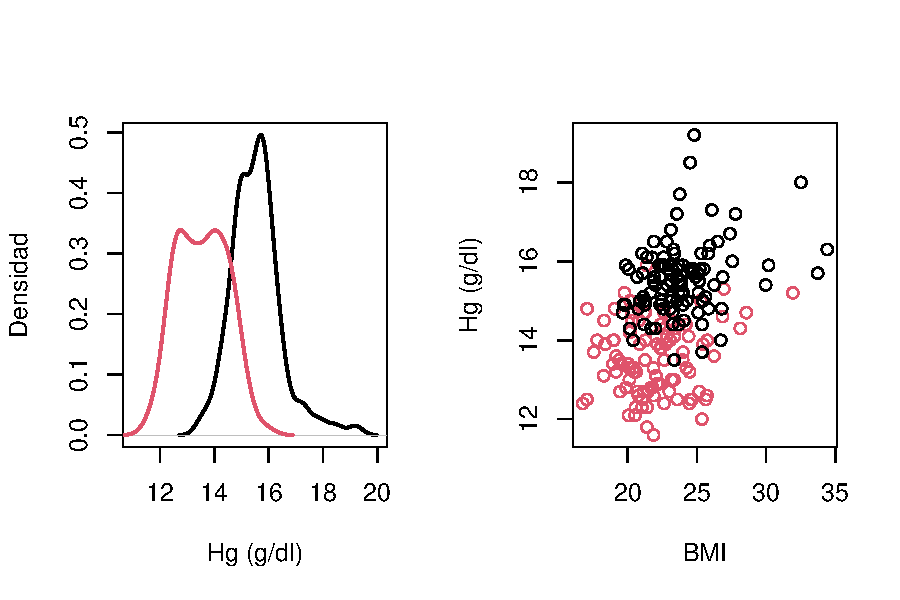
\includegraphics{MLG2_files/figure-latex/AtletesFigure-1} 

}

\caption{Datos de atletas. Densidad de la hemoglobina para hombres y mujeres (derecha) y diagrama de dispersión entre la homoglobina y el índice de masa corporal (izquierda). Negro para hombres y rojo para mujeres.}\label{fig:AtletesFigure}
\end{figure}

En la Figura \ref{fig:AtletesFigure} (izquierda) vemos que los niveles de hemoglobina son mayores para hombres que para mujeres. En la Figura \ref{fig:AtletesFigure} (derecha) observamos que hay una relación positiva entre la hemoglobina y el índice de masa corporal tanto para hombres como para mujeres. Esto nos puede indicar que ingresar el sexo del atleta en el modelo puede mejorarnos el ajuste.

\hypertarget{datos-de-la-onu}{%
\subsubsection{Datos de la ONU}\label{datos-de-la-onu}}

Retomemos los datos de la ONU (\texttt{UN11} de la librería \texttt{alr4}). Las variables de interés son:

\begin{itemize}
\tightlist
\item
  \textbf{fertility}: Número esperado de nacidos vivos por mujer.
\item
  \textbf{ppgdp}: producto nacional bruto per cápita (PNB, en dólares).
\item
  \textbf{Purban}: el porcentaje de la población que vive en un área urbana.
\item
  \textbf{lifeExpF}: esperanza de vida femenina (años).
\item
  \textbf{group}: si el país pertenece a la OCDE (Organización para la Cooperación y el Desarrollo Económicos), África o otros.
\end{itemize}

Por ahora consideremos la relación entre la fertilidad y el PNB per cápita, teniendo en cuenta el grupo al que pertenece cada país.

\begin{Shaded}
\begin{Highlighting}[]
\FunctionTok{data}\NormalTok{(UN11)}
\FunctionTok{plot}\NormalTok{(}\FunctionTok{log}\NormalTok{(fertility)}\SpecialCharTok{\textasciitilde{}}\FunctionTok{log}\NormalTok{(ppgdp),}\AttributeTok{data=}\NormalTok{UN11,}\AttributeTok{col=}\NormalTok{UN11}\SpecialCharTok{$}\NormalTok{group,}\AttributeTok{xlab=}\StringTok{\textquotesingle{}log PNB per cápita (dólares)\textquotesingle{}}\NormalTok{, }\AttributeTok{ylab=}\StringTok{\textquotesingle{}log \# esperado de nacidos vivos por mujer\textquotesingle{}}\NormalTok{)}
\end{Highlighting}
\end{Shaded}

\begin{figure}

{\centering 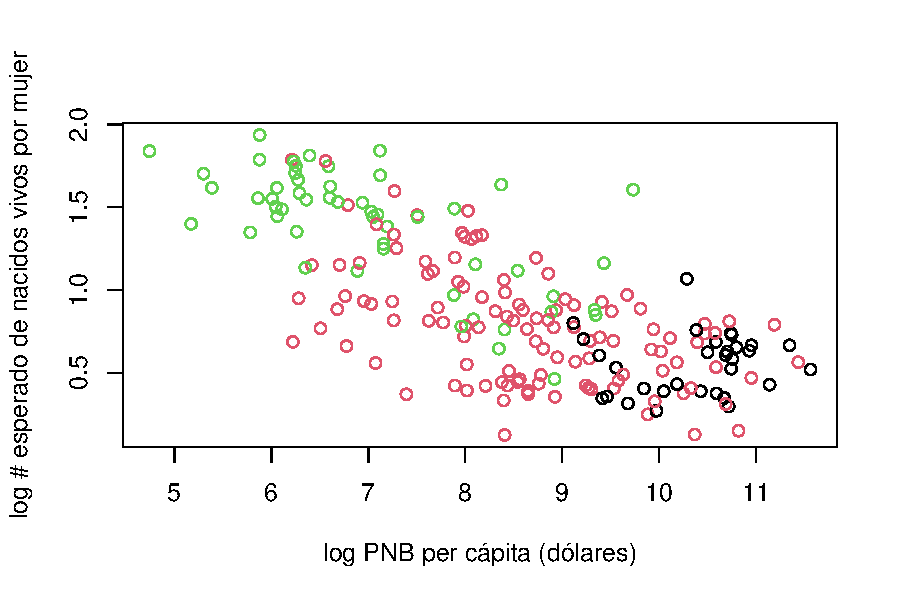
\includegraphics{MLG2_files/figure-latex/UN11Figure-1} 

}

\caption{Datos de la ONU. Relación entre la fertilidad y el PNB per cápita para los países de OCDE (puntos negros), países africanos (puntos verdes) y los otros países (rojos)}\label{fig:UN11Figure}
\end{figure}

En la Figura \ref{fig:UN11Figure} podemos observar que, en general, cuando el PNB aumenta, la tasa de fertilidad disminuye. Sin embargo, esta relación puede variar según la categoría del país. Para los países de la OCDE, esta relación no es fuerte. Mientras que para los demás se mantiene esta relación negativa. Por esta razón sería de gran importancia incluir esta variable categórica dentro del modelo.

\hypertarget{variables-indicadoras}{%
\subsection{Variables indicadoras}\label{variables-indicadoras}}

Las covariables categóricas entran en un modelo como variables indicadoras (o también llamadas \emph{dummies}). En el caso que la covariable \((X)\) tenga dos categorías, entonces se crea una variable indicadora. Por ejemplo, para los datos de los atletas, el sexo requiere una indicadora:
\[
u_{i} = \begin{cases}
1 & \mbox{ si la observación i es hombre}, \\
0 & \mbox{ si la observación i es mujer}. \\
\end{cases}
\]
Aquí mujer es llamada la categoría de referencia.

En caso que la covariable categórica tenga \(k\) categorías, se tienen que crear \(k-1\) variables indicadoras. Por ejemplo, para la variable grupo de país en los datos de la ONU se requieren 2 variables indicadoras \((u_{j})\) como lo muestra la Tabla \ref{tab:dosIndica}.

\begin{table}

\caption{\label{tab:dosIndica}Variables indicadoras para la variable ``group`` de los datos de la ONU}
\centering
\begin{tabular}[t]{lrr}
\toprule
Categoría & $u_{1}$ & $u_{2}$\\
\midrule
OECD & 0 & 0\\
otro & 1 & 0\\
África & 0 & 1\\
\bottomrule
\end{tabular}
\end{table}

\hypertarget{modelos-con-covariables-categuxf3ricas}{%
\subsubsection{Modelos con covariables categóricas}\label{modelos-con-covariables-categuxf3ricas}}

Suponga que se quiere ajustar un modelo para una variable respuesta \(Y\) en función de dos covariables: una continua \(X\) y una indicadora \(Z\) (es decir una variable categórica con dos 2 categorías). El modelo propuesto es el siguiente:
\begin{equation}
y_{i}  = \beta_{0} + x_{i}\beta_{1} + z_{i}\beta_{2} + x_{i}z_{i}\beta_{3} + \varepsilon_{i},
\label{eq:modInter}
\end{equation}
donde \(\varepsilon_{i} \sim N(0,\sigma^{2})\).

Tenemos que, si \(z_i=0\):
\[
E(Y | X=x_i, Z=0) = \beta_{0} + x_{i}\beta_{1}.
\]
Mientras que, si \(z_i=1\):
\[
E(Y | X=x_i, Z=1) = (\beta_{0}+\beta_{2}) + x_{i}(\beta_{1}+\beta_{3}).
\]
Por lo que el modelo \eqref{eq:modInter} genera dos rectas, una para cada categoría. \(\beta_2\) indica la diferencia de intercepto entre las dos categorías y \(\beta_3\) la diferencia entre pendientes. En la Figura \ref{fig:Rectas1}(izquierda) se observan las dos rectas que se obtienen a partir de este modelo. Si se elimina la interacción entre variables, se obtienen dos rectas paralelas (Figura \ref{fig:Rectas1}, derecha).

\begin{figure}

{\centering 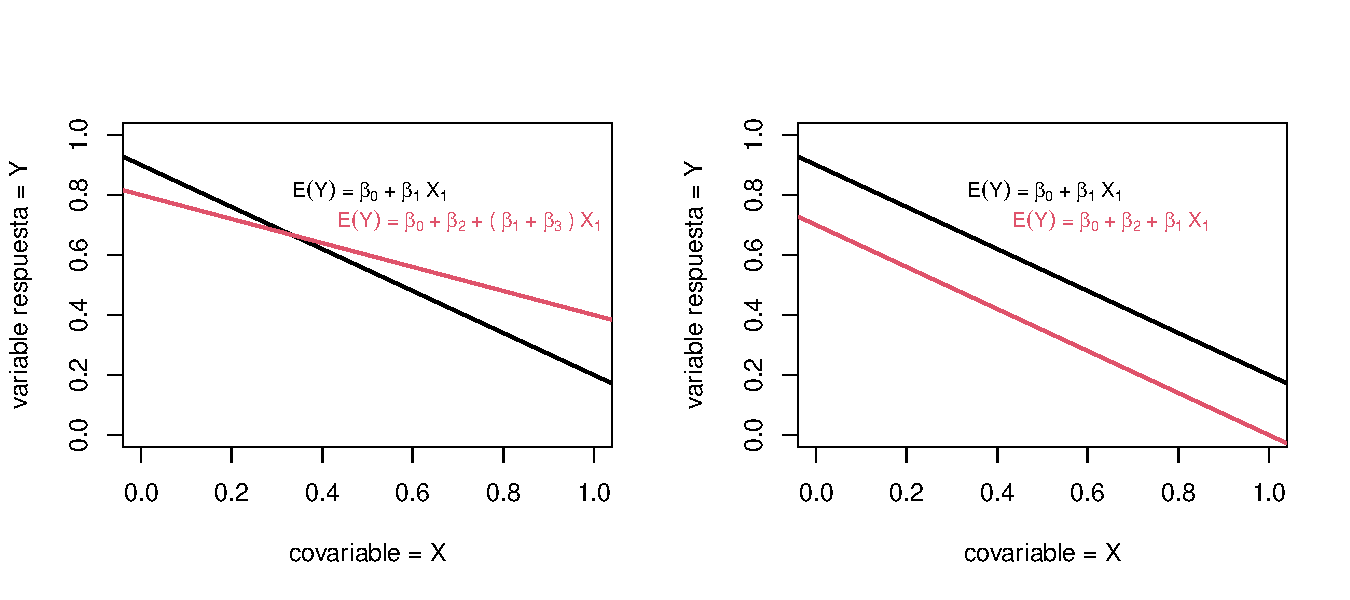
\includegraphics{MLG2_files/figure-latex/Rectas1-1} 

}

\caption{Efecto de la interacción entre variable continua e indicadora. Modelo general (izquierda) y modelo de líneas paralelas (derecha).}\label{fig:Rectas1}
\end{figure}

\hypertarget{modelo-para-los-datos-de-atletas-australianos}{%
\subsubsection{Modelo para los datos de atletas australianos}\label{modelo-para-los-datos-de-atletas-australianos}}

Para los datos de los atletas, se sugiere el siguiente modelo:
\begin{equation}
\begin{split}
\mbox{Hg}_{i} =& \beta_{0} + \mbox{Sex}_{i}\beta_{1} + \mbox{BMI}_{i}\beta_{2} + \mbox{Sex}_{i}\mbox{BMI}_{i}\beta_{3} + \varepsilon_{i},
\end{split}
\nonumber
\end{equation}
donde:
\[
\mbox{Sex}_{i} = \begin{cases}
1 & \mbox{ si la observación i corresponde a una mujer}, \\
0 & \mbox{ de otra forma}. \\
\end{cases}
\]
Note que en la base de datos \texttt{ais}, la variable \texttt{sex} ya está codificada de esta forma. Si la variable no está codificada de forma numérica, \texttt{R} eligirá la categoría de referencia de forma automática.

Para ajustar el modelo utilizamos la función \texttt{lm} (\texttt{Sex*BMI} aquí estamos incluyendo los efectos de \texttt{BMI} y \texttt{Sex}, así como la interacción):

\begin{Shaded}
\begin{Highlighting}[]
\NormalTok{mod.ais }\OtherTok{=} \FunctionTok{lm}\NormalTok{(Hg}\SpecialCharTok{\textasciitilde{}}\NormalTok{Sex}\SpecialCharTok{*}\NormalTok{BMI, }\AttributeTok{data=}\NormalTok{ais)}
\FunctionTok{summary}\NormalTok{(mod.ais)}
\end{Highlighting}
\end{Shaded}

\begin{verbatim}
## 
## Call:
## lm(formula = Hg ~ Sex * BMI, data = ais)
## 
## Residuals:
##     Min      1Q  Median      3Q     Max 
## -1.9997 -0.6625 -0.0478  0.5784  3.5583 
## 
## Coefficients:
##             Estimate Std. Error t value Pr(>|t|)    
## (Intercept) 13.21316    0.78662  16.797   <2e-16 ***
## Sex         -0.66140    1.09835  -0.602   0.5477    
## BMI          0.09788    0.03269   2.994   0.0031 ** 
## Sex:BMI     -0.05203    0.04761  -1.093   0.2758    
## ---
## Signif. codes:  0 '***' 0.001 '**' 0.01 '*' 0.05 '.' 0.1 ' ' 1
## 
## Residual standard error: 0.9092 on 198 degrees of freedom
## Multiple R-squared:  0.5613, Adjusted R-squared:  0.5546 
## F-statistic: 84.44 on 3 and 198 DF,  p-value: < 2.2e-16
\end{verbatim}

Aquí tenemos que \(\widehat{\beta}_{2} =0.1\), lo que nos indica que el valor esperado del nivel de hemoglobina aumenta en \(0.1\) g/dl por cada aumento unitario en el índice de masa corporal de los hombres. Para las mujeres, el efecto del índice de masa corporal sobre el nivel de hemoglobina también es positivo, pero con una pendiente menor \(\widehat{\beta}_{2} +\widehat{\beta}_{3} = -0.66 - 0.1 = -0.56\).

La representación gráfica del modelo se puede observar en la Figura \ref{fig:AtletesAjuste}. Aquí vemos que la pendiente para las mujeres es un poco menor que para los hombres.

\begin{Shaded}
\begin{Highlighting}[]
\FunctionTok{plot}\NormalTok{(Hg}\SpecialCharTok{\textasciitilde{}}\NormalTok{BMI,}\AttributeTok{data=}\NormalTok{ais,}\AttributeTok{col=}\NormalTok{ais}\SpecialCharTok{$}\NormalTok{Sex}\SpecialCharTok{+}\DecValTok{1}\NormalTok{,}\AttributeTok{ylab=}\StringTok{\textquotesingle{}Hg (g/dl)\textquotesingle{}}\NormalTok{,}\AttributeTok{xlab=}\StringTok{\textquotesingle{}BMI\textquotesingle{}}\NormalTok{)}
\FunctionTok{abline}\NormalTok{(}\AttributeTok{a=}\NormalTok{mod.ais}\SpecialCharTok{$}\NormalTok{coefficients[}\DecValTok{1}\NormalTok{],}\AttributeTok{b=}\NormalTok{mod.ais}\SpecialCharTok{$}\NormalTok{coefficients[}\DecValTok{3}\NormalTok{],}\AttributeTok{lwd=}\DecValTok{2}\NormalTok{)}
\FunctionTok{abline}\NormalTok{(}\AttributeTok{a=}\NormalTok{mod.ais}\SpecialCharTok{$}\NormalTok{coefficients[}\DecValTok{1}\NormalTok{]}\SpecialCharTok{+}\NormalTok{mod.ais}\SpecialCharTok{$}\NormalTok{coefficients[}\DecValTok{2}\NormalTok{],}\AttributeTok{b=}\NormalTok{mod.ais}\SpecialCharTok{$}\NormalTok{coefficients[}\DecValTok{3}\NormalTok{]}\SpecialCharTok{+}\NormalTok{mod.ais}\SpecialCharTok{$}\NormalTok{coefficients[}\DecValTok{4}\NormalTok{],}\AttributeTok{col=}\DecValTok{2}\NormalTok{,}\AttributeTok{lwd=}\DecValTok{2}\NormalTok{)}
\end{Highlighting}
\end{Shaded}

\begin{figure}

{\centering 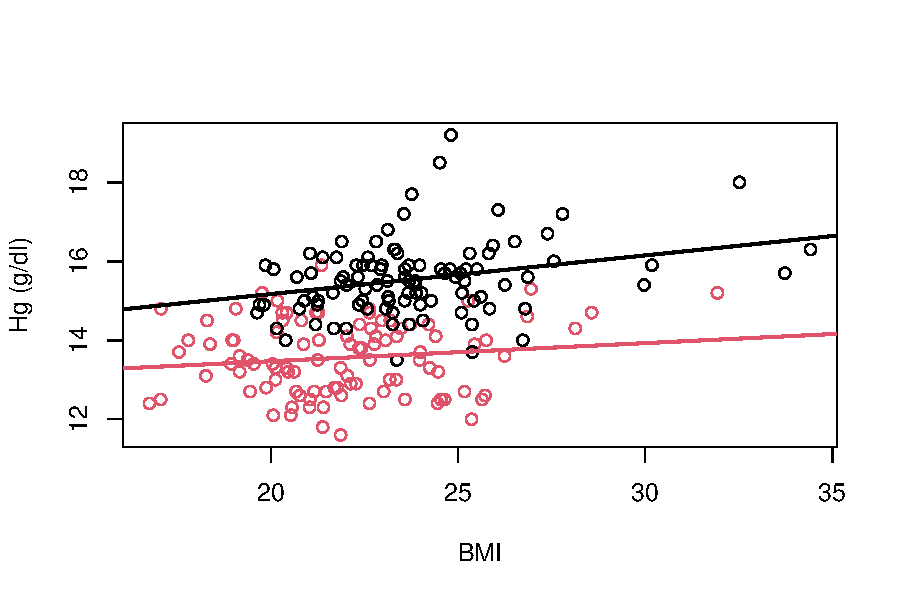
\includegraphics{MLG2_files/figure-latex/AtletesAjuste-1} 

}

\caption{Datos de atletas. Ajuste del modelo para la homoglobina en función  del índice de masa corporal y sexo. Línea negra para hombres y línea roja para mujeres.}\label{fig:AtletesAjuste}
\end{figure}

Si miramos la significancia del \(\widehat{\beta}_3\) (valor-\(p\) igual a 0.276), podemos concluir que las diferencias en pendiente no son significativas. Por lo que, el efecto del índice de masa corporal sobre los niveles de hemoglobina es el mismo para mujeres que para hombres.

Si queremos evaluar si hay diferencias entre hombres y mujeres, debemos evaluar la siguiente hipótesis:
\[
H_{0}: \beta_{1} = \beta_3 = 0.
\]
En \texttt{R}, esto lo podemos realizar usando la función \texttt{anova()} (prueba F) comparando el modelo completo contra el modelo reducido (sin la variable \texttt{Sex}):

\begin{Shaded}
\begin{Highlighting}[]
\NormalTok{mod.ais.red }\OtherTok{=} \FunctionTok{lm}\NormalTok{(Hg}\SpecialCharTok{\textasciitilde{}}\NormalTok{BMI, }\AttributeTok{data=}\NormalTok{ais)}
\FunctionTok{anova}\NormalTok{(mod.ais.red,mod.ais)}
\end{Highlighting}
\end{Shaded}

\begin{verbatim}
## Analysis of Variance Table
## 
## Model 1: Hg ~ BMI
## Model 2: Hg ~ Sex * BMI
##   Res.Df    RSS Df Sum of Sq      F    Pr(>F)    
## 1    200 318.52                                  
## 2    198 163.69  2    154.82 93.637 < 2.2e-16 ***
## ---
## Signif. codes:  0 '***' 0.001 '**' 0.01 '*' 0.05 '.' 0.1 ' ' 1
\end{verbatim}

Aquí vemos que se rechaza \(H_0\) por lo que hay diferencias en la relación de la homoglobina y el índice de masa corporal entre hombres y mujeres (\(\beta_1\) o \(\beta_3\) es diferente de cero, pero no ambos).

El modelo con lineas paralelas es:
\[
\mbox{Hg}_{i} = \beta_{0} + \mbox{Sex}_{i}\beta_{1} + \mbox{BMI}_{i}\beta_{2} +  \varepsilon_{i},
\]
donde \(\varepsilon_{i} \sim N(0, \sigma^{2})\), y se calcula de la siguiente forma:

\begin{Shaded}
\begin{Highlighting}[]
\NormalTok{mod.ais.lp }\OtherTok{=} \FunctionTok{lm}\NormalTok{(Hg}\SpecialCharTok{\textasciitilde{}}\NormalTok{Sex}\SpecialCharTok{+}\NormalTok{BMI, }\AttributeTok{data=}\NormalTok{ais)}
\FunctionTok{summary}\NormalTok{(mod.ais.lp)}
\end{Highlighting}
\end{Shaded}

\begin{verbatim}
## 
## Call:
## lm(formula = Hg ~ Sex + BMI, data = ais)
## 
## Residuals:
##     Min      1Q  Median      3Q     Max 
## -2.0131 -0.6530 -0.0263  0.6249  3.5806 
## 
## Coefficients:
##             Estimate Std. Error t value Pr(>|t|)    
## (Intercept) 13.79954    0.57549  23.979  < 2e-16 ***
## Sex         -1.85251    0.13587 -13.634  < 2e-16 ***
## BMI          0.07335    0.02378   3.085  0.00233 ** 
## ---
## Signif. codes:  0 '***' 0.001 '**' 0.01 '*' 0.05 '.' 0.1 ' ' 1
## 
## Residual standard error: 0.9097 on 199 degrees of freedom
## Multiple R-squared:  0.5586, Adjusted R-squared:  0.5542 
## F-statistic: 125.9 on 2 and 199 DF,  p-value: < 2.2e-16
\end{verbatim}

La estimación del efecto asociado al sexo indica la diferencia media del nivel de hemoglobina entre hombres y mujeres. En la Figura \ref{fig:AtletesAjuste2} vemos que el modelo de líneas paralelas tiene casi el mismo ajuste que el modelo general.

\begin{Shaded}
\begin{Highlighting}[]
\FunctionTok{plot}\NormalTok{(Hg}\SpecialCharTok{\textasciitilde{}}\NormalTok{BMI,}\AttributeTok{data=}\NormalTok{ais,}\AttributeTok{col=}\NormalTok{ais}\SpecialCharTok{$}\NormalTok{Sex}\SpecialCharTok{+}\DecValTok{1}\NormalTok{,}\AttributeTok{ylab=}\StringTok{\textquotesingle{}Hg (g/dl)\textquotesingle{}}\NormalTok{,}\AttributeTok{xlab=}\StringTok{\textquotesingle{}BMI\textquotesingle{}}\NormalTok{)}
\FunctionTok{abline}\NormalTok{(}\AttributeTok{a=}\NormalTok{mod.ais}\SpecialCharTok{$}\NormalTok{coefficients[}\DecValTok{1}\NormalTok{],}\AttributeTok{b=}\NormalTok{mod.ais}\SpecialCharTok{$}\NormalTok{coefficients[}\DecValTok{3}\NormalTok{],}\AttributeTok{lwd=}\DecValTok{2}\NormalTok{)}
\FunctionTok{abline}\NormalTok{(}\AttributeTok{a=}\NormalTok{mod.ais}\SpecialCharTok{$}\NormalTok{coefficients[}\DecValTok{1}\NormalTok{]}\SpecialCharTok{+}\NormalTok{mod.ais}\SpecialCharTok{$}\NormalTok{coefficients[}\DecValTok{2}\NormalTok{],}\AttributeTok{b=}\NormalTok{mod.ais}\SpecialCharTok{$}\NormalTok{coefficients[}\DecValTok{3}\NormalTok{]}\SpecialCharTok{+}\NormalTok{mod.ais}\SpecialCharTok{$}\NormalTok{coefficients[}\DecValTok{4}\NormalTok{],}\AttributeTok{col=}\DecValTok{2}\NormalTok{,}\AttributeTok{lwd=}\DecValTok{2}\NormalTok{)}
\FunctionTok{abline}\NormalTok{(}\AttributeTok{a=}\NormalTok{mod.ais.lp}\SpecialCharTok{$}\NormalTok{coefficients[}\DecValTok{1}\NormalTok{],}\AttributeTok{b=}\NormalTok{mod.ais.lp}\SpecialCharTok{$}\NormalTok{coefficients[}\DecValTok{3}\NormalTok{],}\AttributeTok{lwd=}\DecValTok{2}\NormalTok{,}\AttributeTok{lty=}\DecValTok{2}\NormalTok{)}
\FunctionTok{abline}\NormalTok{(}\AttributeTok{a=}\NormalTok{mod.ais.lp}\SpecialCharTok{$}\NormalTok{coefficients[}\DecValTok{1}\NormalTok{]}\SpecialCharTok{+}\NormalTok{mod.ais.lp}\SpecialCharTok{$}\NormalTok{coefficients[}\DecValTok{2}\NormalTok{],}\AttributeTok{b=}\NormalTok{mod.ais.lp}\SpecialCharTok{$}\NormalTok{coefficients[}\DecValTok{3}\NormalTok{],}\AttributeTok{col=}\DecValTok{2}\NormalTok{,}\AttributeTok{lwd=}\DecValTok{2}\NormalTok{,}\AttributeTok{lty=}\DecValTok{2}\NormalTok{)}
\end{Highlighting}
\end{Shaded}

\begin{figure}

{\centering 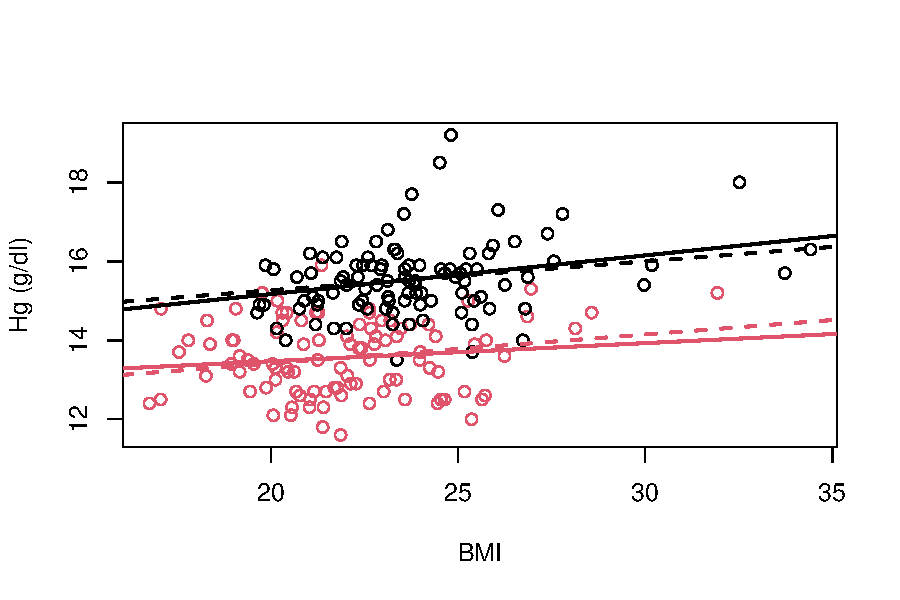
\includegraphics{MLG2_files/figure-latex/AtletesAjuste2-1} 

}

\caption{Datos de atletas. Ajuste del modelo general (línea solida) y el modelo líneas paralelas (línea discontinua) para la homoglobina en función  del índice de masa corporal y sexo. Líneas negra para hombres y líneas roja para mujeres.}\label{fig:AtletesAjuste2}
\end{figure}

\hypertarget{modelo-para-los-datos-de-la-onu}{%
\subsubsection{Modelo para los datos de la ONU}\label{modelo-para-los-datos-de-la-onu}}

El modelo propuesto es el siguiente:
\begin{equation}
\begin{split}
\log\mbox{fertility}_{i} =& \beta_{0} + \mbox{u}_{1i}\beta_{1}+\mbox{u}_{2i}\beta_{2} + \log\mbox{ppgdp}_{i}\beta_{3} + \\ & \mbox{u}_{1i}\log\mbox{ppgdp}_{i}\beta_{4} + \mbox{u}_{2i}\log\mbox{ppgdp}_{i}\beta_{5} + \varepsilon_{i},
\end{split}
\nonumber
\end{equation}
donde:
\[
\mbox{u}_{1i} = \begin{cases}
1 & \mbox{ si el país i pertenece a la categoría otro}, \\
0 & \mbox{ de otra forma}, \\
\end{cases} \quad \mbox{ y } \quad 
\mbox{u}_{2i} = \begin{cases}
1 & \mbox{ si el país i pertenece a África}, \\
0 & \mbox{ de otra forma}. \\
\end{cases}
\]
Por lo tanto, OECD es la categoría de referencia.

El modelo ajustado es:

\begin{Shaded}
\begin{Highlighting}[]
\NormalTok{mod.UN11 }\OtherTok{=} \FunctionTok{lm}\NormalTok{(}\FunctionTok{log}\NormalTok{(fertility)}\SpecialCharTok{\textasciitilde{}}\NormalTok{group}\SpecialCharTok{*}\FunctionTok{log}\NormalTok{(ppgdp), }\AttributeTok{data=}\NormalTok{UN11)}
\FunctionTok{summary}\NormalTok{(mod.UN11)}
\end{Highlighting}
\end{Shaded}

\begin{verbatim}
## 
## Call:
## lm(formula = log(fertility) ~ group * log(ppgdp), data = UN11)
## 
## Residuals:
##      Min       1Q   Median       3Q      Max 
## -0.69358 -0.16963  0.02005  0.16838  0.73633 
## 
## Coefficients:
##                        Estimate Std. Error t value Pr(>|t|)   
## (Intercept)             0.21836    0.81290   0.269  0.78851   
## groupother              1.87888    0.83290   2.256  0.02520 * 
## groupafrica             2.54072    0.84299   3.014  0.00293 **
## log(ppgdp)              0.03217    0.07832   0.411  0.68170   
## groupother:log(ppgdp)  -0.18418    0.08106  -2.272  0.02417 * 
## groupafrica:log(ppgdp) -0.22637    0.08430  -2.685  0.00788 **
## ---
## Signif. codes:  0 '***' 0.001 '**' 0.01 '*' 0.05 '.' 0.1 ' ' 1
## 
## Residual standard error: 0.2739 on 193 degrees of freedom
## Multiple R-squared:  0.6305, Adjusted R-squared:  0.6209 
## F-statistic: 65.86 on 5 and 193 DF,  p-value: < 2.2e-16
\end{verbatim}

A partir de estos resultados obtenemos tres rectas que describen el valor esperado del logarítmo de la fertilidad en función del logarítmo del PNB per cápita, una para cada tipo de país. Para los países de la OCDE, tenemos que:
\[
E(\log\mbox{fertility}) = 0.218 + 0.032\log \mbox{ppgdp}.
\]
Para los países Africanos:
\[
E(\log\mbox{fertility}) = 2.759  -0.194\log \mbox{ppgdp}.
\]
Finalmente, para los otros países:
\[
E(\log\mbox{fertility}) = 2.097  -0.152\log \mbox{ppgdp}.
\]
Aquí vemos que para los países que no son de la OCDE, el producto nacional bruto tiene un efecto significativo negativo sobre la tasa de fertilidad. Mientras que para los países de la OCDE, este efecto es positivo, aunque no es significativo. Esto mismo lo podemos ver gráficamente en la Figura \ref{fig:MCOUN11Figure}.

\begin{Shaded}
\begin{Highlighting}[]
\NormalTok{Beta.UN11 }\OtherTok{=}\NormalTok{ mod.UN11}\SpecialCharTok{$}\NormalTok{coefficients}
\FunctionTok{plot}\NormalTok{(}\FunctionTok{log}\NormalTok{(fertility)}\SpecialCharTok{\textasciitilde{}}\FunctionTok{log}\NormalTok{(ppgdp),}\AttributeTok{data=}\NormalTok{UN11,}\AttributeTok{col=}\NormalTok{UN11}\SpecialCharTok{$}\NormalTok{group,}\AttributeTok{xlab=}\StringTok{\textquotesingle{}log PNB per cápita (dólares)\textquotesingle{}}\NormalTok{, }\AttributeTok{ylab=}\StringTok{\textquotesingle{}log \# esperado de nacidos vivos por mujer\textquotesingle{}}\NormalTok{)}
\FunctionTok{abline}\NormalTok{(}\AttributeTok{a=}\NormalTok{Beta.UN11[}\DecValTok{1}\NormalTok{],}\AttributeTok{b=}\NormalTok{Beta.UN11[}\DecValTok{4}\NormalTok{],}\AttributeTok{lwd=}\DecValTok{2}\NormalTok{)}
\FunctionTok{abline}\NormalTok{(}\AttributeTok{a=}\NormalTok{Beta.UN11[}\DecValTok{1}\NormalTok{]}\SpecialCharTok{+}\NormalTok{Beta.UN11[}\DecValTok{2}\NormalTok{],}\AttributeTok{b=}\NormalTok{Beta.UN11[}\DecValTok{4}\NormalTok{]}\SpecialCharTok{+}\NormalTok{Beta.UN11[}\DecValTok{5}\NormalTok{],}\AttributeTok{col=}\DecValTok{2}\NormalTok{,}\AttributeTok{lwd=}\DecValTok{2}\NormalTok{)}
\FunctionTok{abline}\NormalTok{(}\AttributeTok{a=}\NormalTok{Beta.UN11[}\DecValTok{1}\NormalTok{]}\SpecialCharTok{+}\NormalTok{Beta.UN11[}\DecValTok{3}\NormalTok{],}\AttributeTok{b=}\NormalTok{Beta.UN11[}\DecValTok{4}\NormalTok{]}\SpecialCharTok{+}\NormalTok{Beta.UN11[}\DecValTok{6}\NormalTok{],}\AttributeTok{col=}\DecValTok{3}\NormalTok{,}\AttributeTok{lwd=}\DecValTok{2}\NormalTok{)}
\end{Highlighting}
\end{Shaded}

\begin{figure}

{\centering 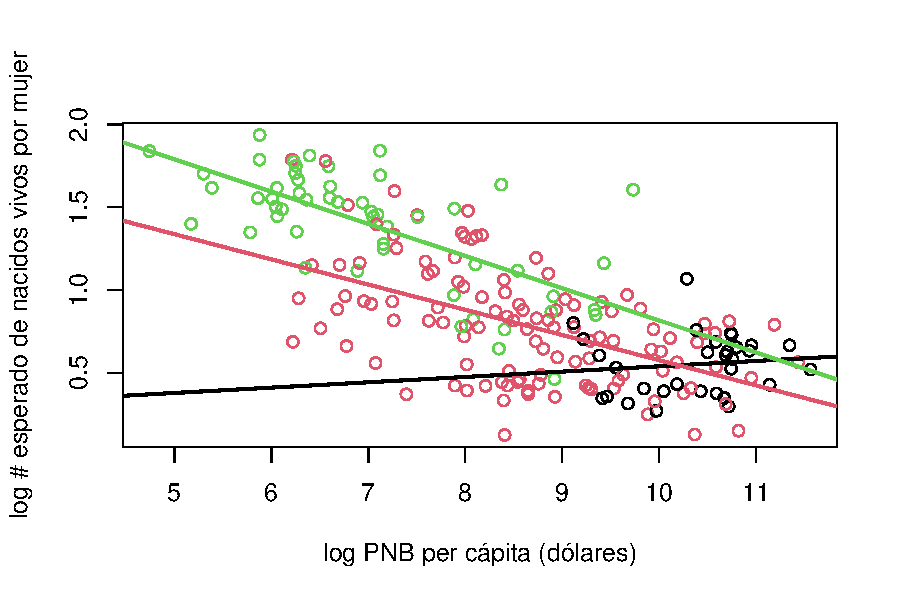
\includegraphics{MLG2_files/figure-latex/MCOUN11Figure-1} 

}

\caption{Datos de la ONU. Ajuste del modelo para la fertilidad en función  del PNB y tipo de país. Países de OCDE (línea negra), países africanos (línea verde) y los otros países (línea roja)}\label{fig:MCOUN11Figure}
\end{figure}

Usando la función \texttt{relevel()} se puede cambiar la categoría de referencia. Por ejemplo, si queremos que la categoría de referencia sea \texttt{other}:

\begin{Shaded}
\begin{Highlighting}[]
\NormalTok{UN11.alt }\OtherTok{=}\NormalTok{ UN11}
\NormalTok{UN11.alt}\SpecialCharTok{$}\NormalTok{group }\OtherTok{=}  \FunctionTok{relevel}\NormalTok{(UN11.alt}\SpecialCharTok{$}\NormalTok{group,}\AttributeTok{ref =}\StringTok{\textquotesingle{}other\textquotesingle{}}\NormalTok{)}
\NormalTok{mod.UN11.alt }\OtherTok{=} \FunctionTok{lm}\NormalTok{(}\FunctionTok{log}\NormalTok{(fertility)}\SpecialCharTok{\textasciitilde{}}\NormalTok{group}\SpecialCharTok{*}\FunctionTok{log}\NormalTok{(ppgdp), }\AttributeTok{data=}\NormalTok{UN11.alt)}
\FunctionTok{summary}\NormalTok{(mod.UN11.alt)}
\end{Highlighting}
\end{Shaded}

Cambiar la categoría de referencia no cambia en nada los resultados del ajuste. Solo cambian la interpretación de los coeficientes.

Se podría hacer la siguiente pregunta, ¿el efecto del PNB sobre la fertilidad es el mismo para cada tipo de país?. Para resolver esta pregunta, se plantea la siguiente hipótesis:
\[
H_0: \beta_4 = \beta_5 = 0.
\]
Usando la función \texttt{anova()} (prueba F) en R:

\begin{Shaded}
\begin{Highlighting}[]
\NormalTok{mod.UN11.red }\OtherTok{=} \FunctionTok{lm}\NormalTok{(}\FunctionTok{log}\NormalTok{(fertility)}\SpecialCharTok{\textasciitilde{}}\NormalTok{group}\SpecialCharTok{+}\FunctionTok{log}\NormalTok{(ppgdp), }\AttributeTok{data=}\NormalTok{UN11)}
\FunctionTok{anova}\NormalTok{(mod.UN11.red,mod.UN11)}
\end{Highlighting}
\end{Shaded}

\begin{verbatim}
## Analysis of Variance Table
## 
## Model 1: log(fertility) ~ group + log(ppgdp)
## Model 2: log(fertility) ~ group * log(ppgdp)
##   Res.Df    RSS Df Sum of Sq      F  Pr(>F)  
## 1    195 15.033                              
## 2    193 14.484  2   0.54848 3.6542 0.02769 *
## ---
## Signif. codes:  0 '***' 0.001 '**' 0.01 '*' 0.05 '.' 0.1 ' ' 1
\end{verbatim}

Este resultado indica que hay evidencia suficiente para concluir que el efecto del PNB sobre la fertilidad no es el mismo para cada tipo de país.

Ahora, podríamos preguntarnos: ¿las pendientes son las mismas para las categorías de otro y África?. Para esto, se plantea la siguiente hipótesis:
\[
H_0: \beta_4 = \beta_5.
\]
También se puede expresar de la siguiente forma:
\[
H_{0}: \boldsymbol L\boldsymbol \beta= \begin{pmatrix}
0 & 0 & 0 & 0 & 1 & -1
\end{pmatrix} \begin{pmatrix}
\beta_0 \\ \beta_1 \\ \beta_2 \\ \beta_3 \\ \beta_4 \\ \beta_5
\end{pmatrix} = 0
\]
Esto, en R es:

\begin{Shaded}
\begin{Highlighting}[]
\NormalTok{L }\OtherTok{=} \FunctionTok{matrix}\NormalTok{(}\FunctionTok{c}\NormalTok{(}\DecValTok{0}\NormalTok{,}\DecValTok{0}\NormalTok{,}\DecValTok{0}\NormalTok{,}\DecValTok{0}\NormalTok{,}\DecValTok{1}\NormalTok{,}\SpecialCharTok{{-}}\DecValTok{1}\NormalTok{),}\DecValTok{1}\NormalTok{,}\DecValTok{6}\NormalTok{,}\AttributeTok{byrow =}\NormalTok{ T)}
\FunctionTok{linearHypothesis}\NormalTok{(mod.UN11, }\AttributeTok{hypothesis.matrix=}\NormalTok{L)}
\end{Highlighting}
\end{Shaded}

\begin{verbatim}
## Linear hypothesis test
## 
## Hypothesis:
## groupother:log(ppgdp) - groupafrica:log(ppgdp) = 0
## 
## Model 1: restricted model
## Model 2: log(fertility) ~ group * log(ppgdp)
## 
##   Res.Df    RSS Df Sum of Sq      F Pr(>F)
## 1    194 14.579                           
## 2    193 14.484  1  0.094808 1.2633 0.2624
\end{verbatim}

Dado que no se rechaza \(H_0\), el efecto del PNB sobre la fertilidad es el mismo para los países Africano y los de la categoría de otros.

En resumen, a partir del análisis de regresión:
- El efecto del PNB per cápita es diferente cada tipo de país.
- Para los países miembros de la OECD, el efecto es positivo (aunque no es significativo).
- Para los países de áfrica y otros, el efecto es negativo (y no es significativamente diferente).

\hypertarget{modelos-polinomiales}{%
\section{Modelos polinomiales}\label{modelos-polinomiales}}

\hypertarget{ejemplos-1}{%
\subsection{Ejemplos}\label{ejemplos-1}}

\hypertarget{pasteles}{%
\subsubsection{Pasteles}\label{pasteles}}

Con los datos \texttt{cakes} de la libreria \texttt{alr4} se tienen dos objetivos. Primero, evaluar el efecto de la temperatura y tiempo de horneado sobre la palatabilidad de mazclas de pasteles para hornear. Segundo, encontrar la combinación de estos factores que maximizan la palatabilidad.

Como variable respuesta (\texttt{Y}) se tiene el promedio de calificación de la palatabilidad de cuatro pasteles horneados. Mientras que las covariables son: el tiempo de horneado (\texttt{X1}, en minutos) y la temperatura (\texttt{X2}, en grados Fahrenheit)

\begin{Shaded}
\begin{Highlighting}[]
\FunctionTok{library}\NormalTok{(alr4)}
\FunctionTok{data}\NormalTok{(cakes)}
\FunctionTok{plot}\NormalTok{(cakes[,}\SpecialCharTok{{-}}\DecValTok{1}\NormalTok{])}
\end{Highlighting}
\end{Shaded}

\begin{figure}

{\centering 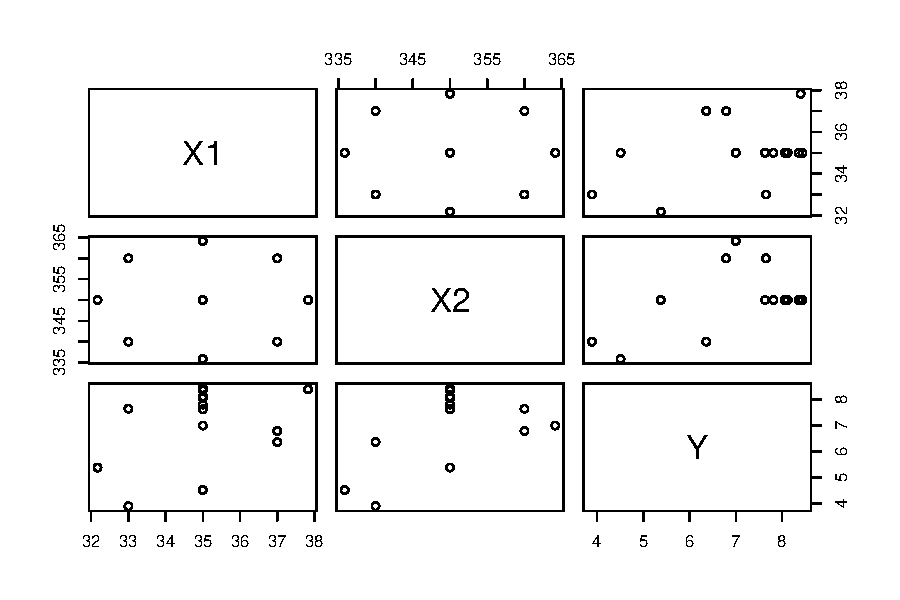
\includegraphics{MLG2_files/figure-latex/CakesFigure-1} 

}

\caption{Datos de pasteles. Diagrama de dispersión.}\label{fig:CakesFigure}
\end{figure}

\hypertarget{datos-de-boston}{%
\subsubsection{Datos de Boston}\label{datos-de-boston}}

La base de datos \texttt{Boston} de la libreria \texttt{MASS} contiene información sobre 506 suburbios del area metropolitana de Boston. El objetivo del estudio es evaluar la relación del precio de las viviendas y la concentración de contaminación ambienta. En esta sección evaluaremos la relación entre la concentración anual de óxido de nitrógeno (\(y\), en partes por diez millones) y la distancia a cinco centros de empleo.

\begin{Shaded}
\begin{Highlighting}[]
\FunctionTok{library}\NormalTok{(MASS)}
\FunctionTok{data}\NormalTok{(Boston)}
\FunctionTok{plot}\NormalTok{(nox}\SpecialCharTok{\textasciitilde{}}\NormalTok{dis,}\AttributeTok{data=}\NormalTok{Boston,}\AttributeTok{ylab=}\StringTok{\textquotesingle{}NOx\textquotesingle{}}\NormalTok{,}\AttributeTok{xlab=}\StringTok{\textquotesingle{}distancia a centros de empleo\textquotesingle{}}\NormalTok{)}
\end{Highlighting}
\end{Shaded}

\begin{figure}

{\centering 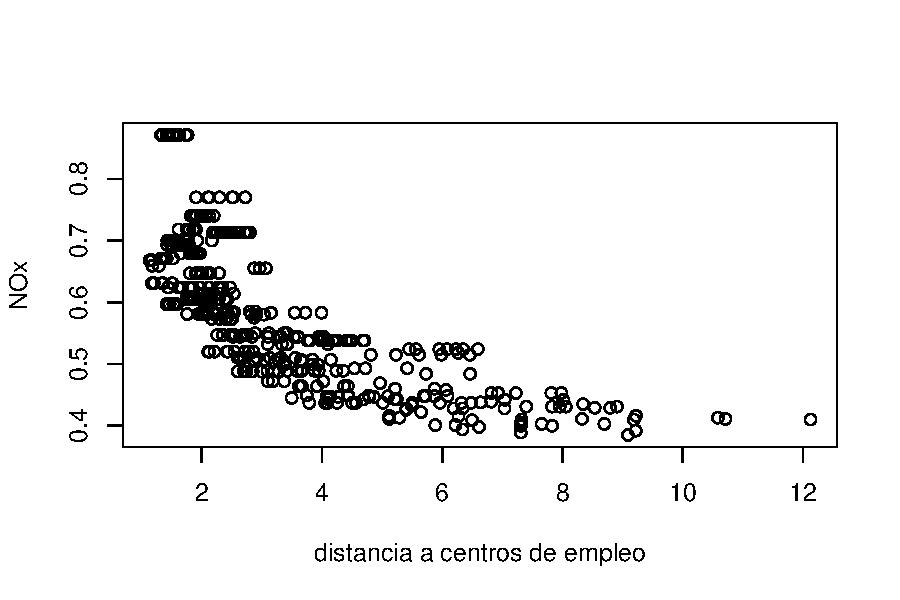
\includegraphics{MLG2_files/figure-latex/BostonFigure-1} 

}

\caption{Datos de Boston. Relación entre el óxido de nitrógeno y la distancia a centros de empleo.}\label{fig:BostonFigure}
\end{figure}

\hypertarget{modelos-polinomiales-1}{%
\subsection{Modelos polinomiales}\label{modelos-polinomiales-1}}

El modelo:
\[
y_{i} = \beta_{0} + \beta_{1}x_{i} + \varepsilon_i,
\]

describe la relación lineal entre \(y\) y \(x_1\). Si las relación entre las variables presentan curvaturas, se puede considerar un modelo polinómico de la forma:
\[
y_{i} = \beta_{0} + \beta_{1}x_{i} + \beta_{2}x_{i}^{2} + \ldots + + \beta_{k}x_{i}^{k} + \varepsilon_i.
\]
Este modelo se sigue considerando como un modelo lineal, dado que es lineal en los parámetros \(\boldsymbol \beta\). En la Figura \ref{fig:Polinomios} se puede observar diferentes curvas para modelos lineales (orden 1), cuadráticos (orden 2) y cúbicos (orden 3). Aquí vemos que este tipo de modelos son muy versatiles. Caulquier función suave se puede ajustar meidante un polinomio de grado suficientemente alto. Por esta razón, los modelos polinomicos son usados en casos donde las relaciones entre las variables son no-lineales y se pueden aproximar por un polinomio.

\begin{figure}

{\centering 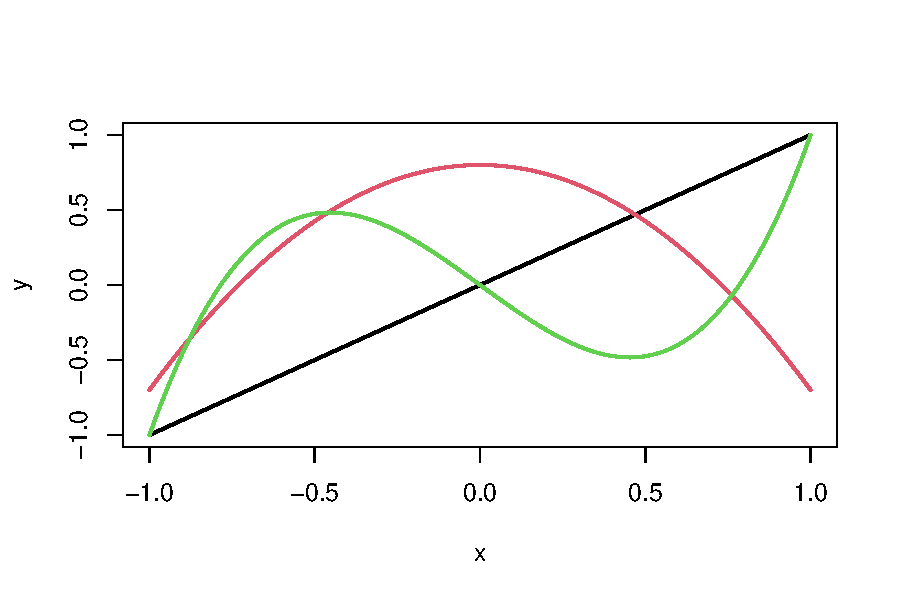
\includegraphics{MLG2_files/figure-latex/Polinomios-1} 

}

\caption{Polinomio de grado 1 (linea negra), grado 2 (linea roja) y grado 3 (linea verde).}\label{fig:Polinomios}
\end{figure}

En el caso que se tengan dos covariables, un modelo de orden 2 se expresa de la forma:
\[
y_{i} = \beta_{0} + \beta_{1}x_{1i} + \beta_{2}x_{2i} + \beta_{3}x_{1i}^2 + \beta_{4}x_{2i}^2 + \beta_{5}x_{1i}x_{2i} + \varepsilon_i.
\]
En las Figuras \ref{fig:modPoli1}-\ref{fig:modPoli3} muestran el valor esperado de \(Y\) en un modelo lineal (asumiendo \(\beta_3=\beta_4=\beta_5=0\)), cuadrático y con interacción (asumiendo \(\beta_3=\beta_4=0\)).

\begin{figure}

{\centering 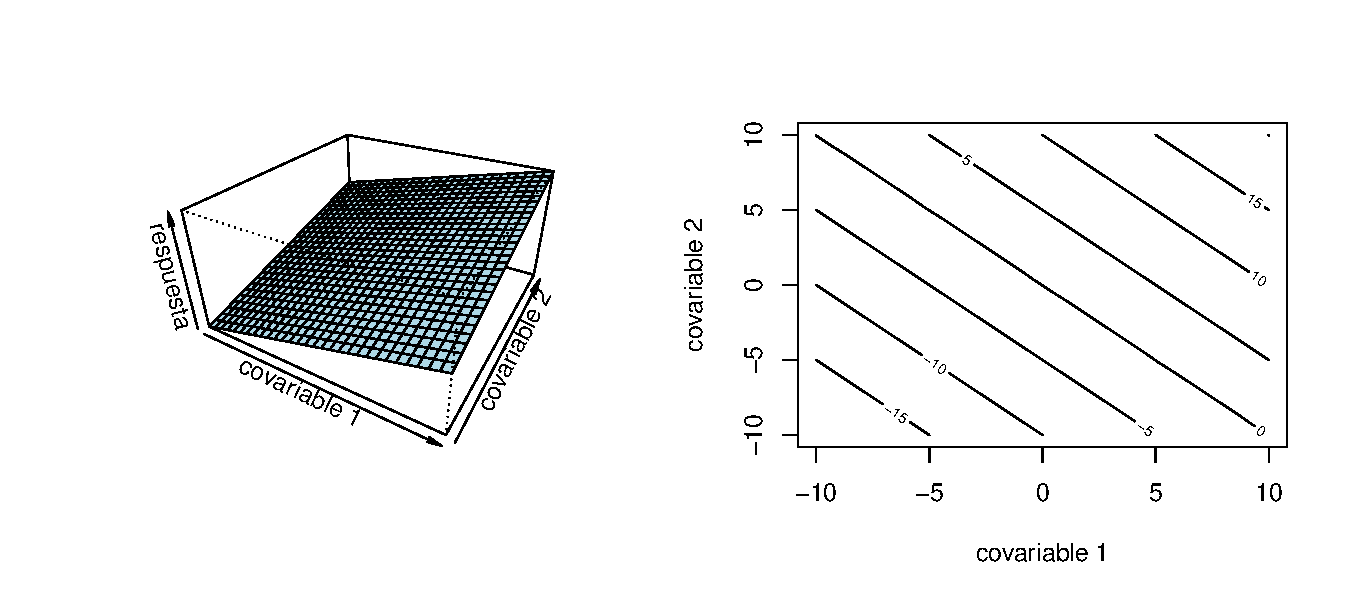
\includegraphics{MLG2_files/figure-latex/modPoli1-1} 

}

\caption{Valor esperado de $Y$ en un modelo lineal (izquierda) y gráfico de contorno (derecha).}\label{fig:modPoli1}
\end{figure}

El número de parámetros incrementa rápidamente con el número de covariables. Con \(k\) covariables, tenemos: un intercepto, \(k\) términos lineales, \(k\)
términos cuadráticos, y \(k(k - 1)/2\) interacciones. Por esta razón, en muchos casos, no se toman en cuentas las interacción cuando el número de covariables es grande.

\begin{figure}

{\centering 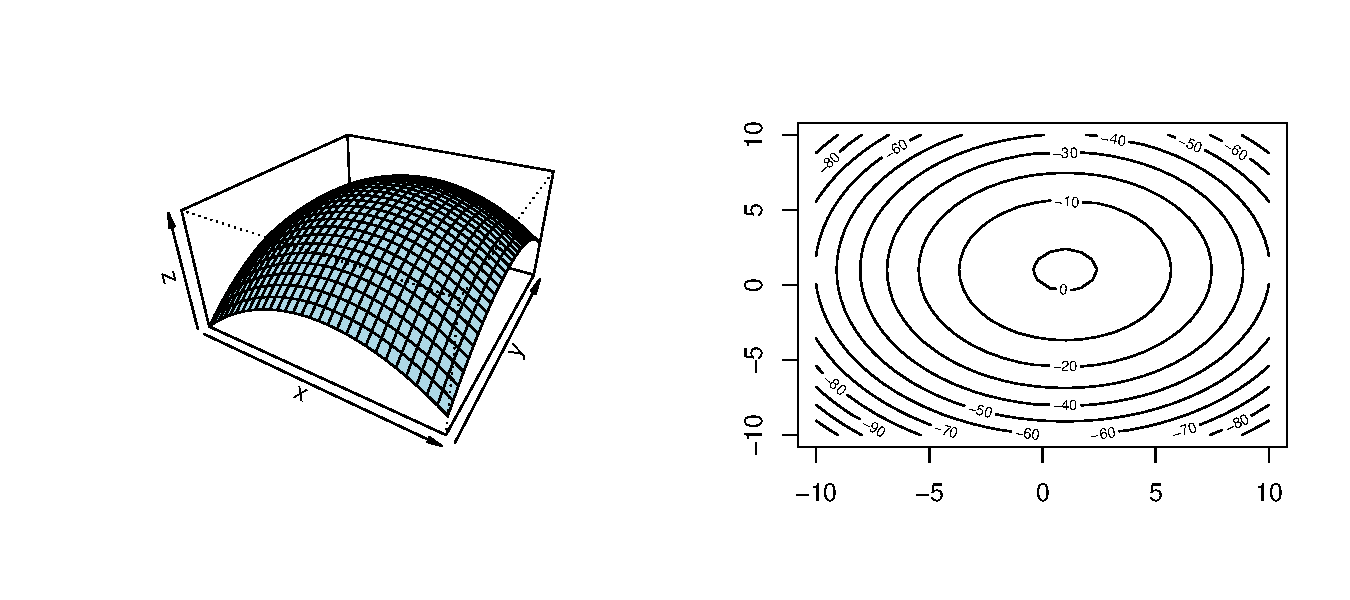
\includegraphics{MLG2_files/figure-latex/modPoli2-1} 

}

\caption{Valor esperado de $Y$ en un modelo cuadrático (izquierda) y gráfico de contorno (derecha).}\label{fig:modPoli2}
\end{figure}

\begin{figure}

{\centering 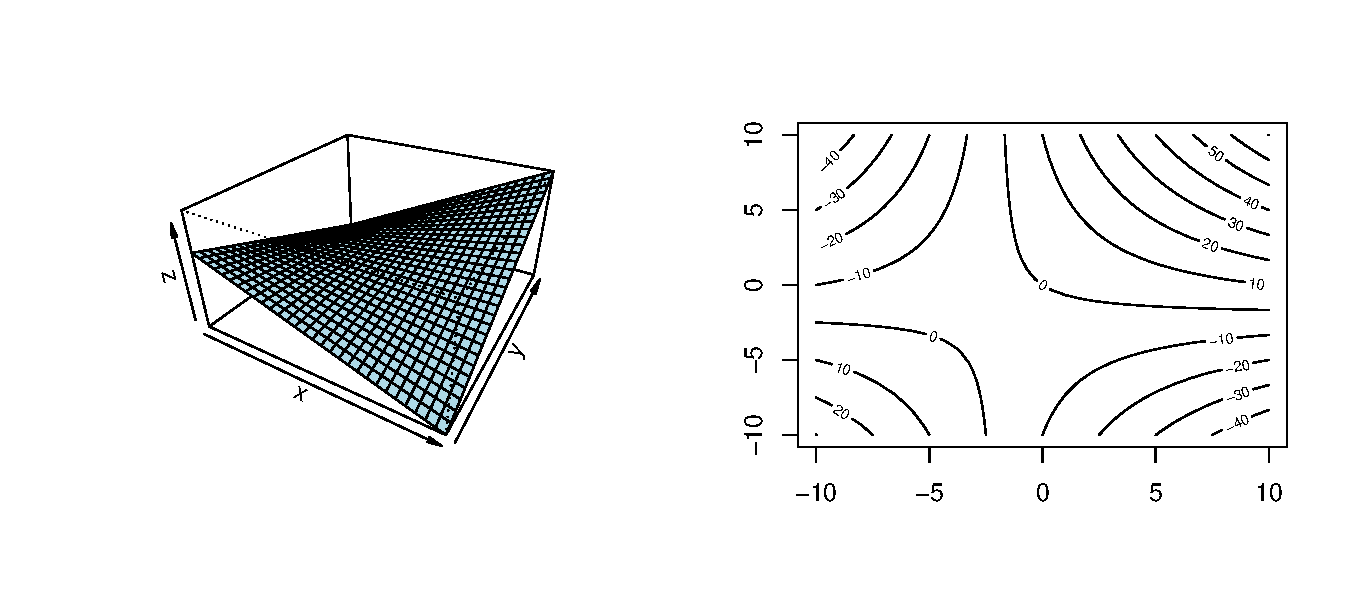
\includegraphics{MLG2_files/figure-latex/modPoli3-1} 

}

\caption{Valor esperado de $Y$ en un modelo lineal con interacción (izquierda) y gráfico de contorno (derecha).}\label{fig:modPoli3}
\end{figure}

Hay aspectos que se deben tener en la práctica cuando se implementa un modelo polinomial:

\begin{itemize}
\tightlist
\item
  \textbf{Selección del orden:} La idea es mantener el orden del polinomio bajo. Si embargo, si es muy bajo no logra capturar la curvatura presente en los datos. En caso que el orden sea grande, el modelo es innecesariamente más complejo y puede haber problemas de multicolinealidad.
\end{itemize}

Si los datos exige un modelo de orden alto \((k > 3)\), se pueden hacer transformación sobre las variables, y así, poder ajustar un modelo polinomial de orden bajo (por ejemplo cuadrático).

La selección del orden puede hacerse de dos formas. (1) ** Hacia delante\textbf{: empezar con un modelo de orden \(1\) e incrementar el orden uno a uno hasta que un término mayor ya no sea significativo. }Hacia atrás:** empezar con el modelo más complejo y eliminar los términos mayores uno a uno hasta que todos sean significativos.

\begin{itemize}
\tightlist
\item
  \textbf{Extrapolación}: La extrapolación con modelos polinomiales puede ser muy peligrosa. Por ejemplo en la Figura \ref{fig:extrapolacion} podemos ajustar un modelo de orden dos a los datos (linea negra). Si hacemos una predicción fuera del rango de los datos, el valor esperado predicho sigue el comportamiento cuadrático propuesto. Sin embargo, el valor esperado de \(Y\) puede seguir un comportamiento diferente (linea roja discontinua). Lo que lleva a tener una predicción sesgada.
\end{itemize}

\begin{figure}

{\centering 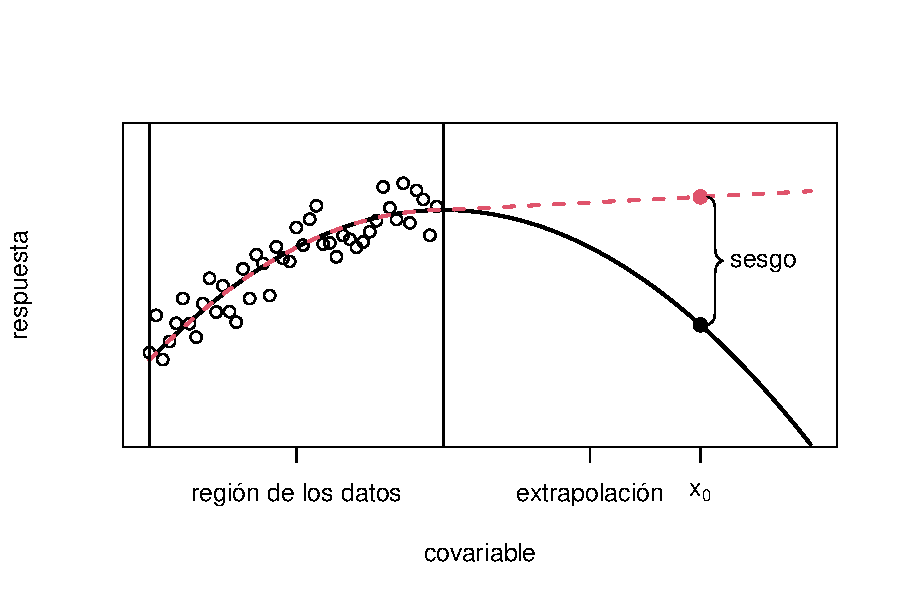
\includegraphics{MLG2_files/figure-latex/extrapolacion-1} 

}

\caption{Problema de extrapolación.}\label{fig:extrapolacion}
\end{figure}

\begin{itemize}
\tightlist
\item
  \textbf{Multicolinealidad}: Al aumentar el polinomio, la matriz \(\boldsymbol X'\boldsymbol X\) se vuelve mal acondicionada. Es decir, las estimaciones pueden ser inestables y los errores estándar se inflan. Este problema se puede solucionar centrando las covariables. Por ejemplo en un modelo de orden 2:
  \[
  E(Y | X=x) = \beta_{0} + \beta_{1}(x-\bar{x}) + \beta_{2}(x-\bar{x})^{2}.
  \]
  Otra solución es usando polinomios ortogonales.
\end{itemize}

\hypertarget{interpretaciuxf3n-de-los-coeficientes}{%
\subsubsection{Interpretación de los coeficientes}\label{interpretaciuxf3n-de-los-coeficientes}}

Considere un modelo de orden 2. El valor esperado de \(Y\) está dado por:
\[
E(Y| X_{1}=x_1,X_{2}=x_2) = \beta_{0} + \beta_{1}x_{1} + \beta_{2}x_{2} + \beta_{3}x_{1}^{2} + \beta_{4}x_{2}^{2} + \beta_{5}x_{1}x_{2}.
\]
Si \(x_{1}\) cambia en \(\delta\) unidades \((x_{1} + \delta)\), tenemos que:
\[
E(Y| X_{1}=x_1+\delta,X_{2}=x_2) =  \beta_{0} + \beta_{1}(x_{1}+\delta) + \beta_{2}x_{2} + \beta_{3}(x_{1} + \delta)^{2} + \beta_{4}x_{2}^{2} + \beta_{5}(x_{1}+\delta)x_{2}.
\]
Ahora calculando la diferencia:
\[
E(Y| X_{1}=x_1+\delta,X_{2}=x_2) - E(Y| X_{1}=x_1,X_{2}=x_2) = (\beta_{1}\delta + \beta_{3}\delta^{2}) + 2\beta_{3}\delta x_{1} + \beta_{5}\delta x_{2}.
\]
Aquí podemos observar que el efecto del cambio \(\delta\) en \(X_1\) depende de ambas covariables y del valor de \(\delta\). Por esta razón es complicado interpretar coeficientes en modelos polinomiales.

\hypertarget{pasteles-1}{%
\subsubsection{Pasteles}\label{pasteles-1}}

Para los datos de los pasteles, se propone el siguiente modelo:
\[
y_{i} = \beta_{0} + \beta_{1}x_{1i} + \beta_{2}x_{2i} + \beta_{3}x_{1i}^2 + \beta_{4}x_{2i}^{2} + \beta_{5}x_{1i}x_{2i} + \varepsilon_{i}.
\]
El ajuste del modelo es:

\begin{Shaded}
\begin{Highlighting}[]
\NormalTok{mod.cakes }\OtherTok{=} \FunctionTok{lm}\NormalTok{(Y }\SpecialCharTok{\textasciitilde{}}\NormalTok{ X1}\SpecialCharTok{*}\NormalTok{X2 }\SpecialCharTok{+} \FunctionTok{I}\NormalTok{(X1}\SpecialCharTok{\^{}}\DecValTok{2}\NormalTok{)}\SpecialCharTok{+}\FunctionTok{I}\NormalTok{(X2}\SpecialCharTok{\^{}}\DecValTok{2}\NormalTok{),}\AttributeTok{data=}\NormalTok{cakes)}
\FunctionTok{summary}\NormalTok{(mod.cakes)}
\end{Highlighting}
\end{Shaded}

\begin{verbatim}
## 
## Call:
## lm(formula = Y ~ X1 * X2 + I(X1^2) + I(X2^2), data = cakes)
## 
## Residuals:
##     Min      1Q  Median      3Q     Max 
## -0.4912 -0.3080  0.0200  0.2658  0.5454 
## 
## Coefficients:
##               Estimate Std. Error t value Pr(>|t|)    
## (Intercept) -2.204e+03  2.416e+02  -9.125 1.67e-05 ***
## X1           2.592e+01  4.659e+00   5.563 0.000533 ***
## X2           9.918e+00  1.167e+00   8.502 2.81e-05 ***
## I(X1^2)     -1.569e-01  3.945e-02  -3.977 0.004079 ** 
## I(X2^2)     -1.195e-02  1.578e-03  -7.574 6.46e-05 ***
## X1:X2       -4.163e-02  1.072e-02  -3.883 0.004654 ** 
## ---
## Signif. codes:  0 '***' 0.001 '**' 0.01 '*' 0.05 '.' 0.1 ' ' 1
## 
## Residual standard error: 0.4288 on 8 degrees of freedom
## Multiple R-squared:  0.9487, Adjusted R-squared:  0.9167 
## F-statistic:  29.6 on 5 and 8 DF,  p-value: 5.864e-05
\end{verbatim}

Además, los factores de inflación de varianza son los siguientes:

\begin{Shaded}
\begin{Highlighting}[]
\NormalTok{car}\SpecialCharTok{::}\FunctionTok{vif}\NormalTok{(mod.cakes)}
\end{Highlighting}
\end{Shaded}

\begin{verbatim}
##       X1       X2  I(X1^2)  I(X2^2)    X1:X2 
## 3778.083 5921.833 1328.089 5309.339 3063.500
\end{verbatim}

Aquí vemos que los VIF presentan valores muy altos, producto de ajustar un modelo cuadrático. Ahora consideremos el modelo con las covariables centradas:

\begin{Shaded}
\begin{Highlighting}[]
\NormalTok{cakes}\SpecialCharTok{$}\NormalTok{X1c }\OtherTok{=}\NormalTok{ cakes}\SpecialCharTok{$}\NormalTok{X1 }\SpecialCharTok{{-}} \FunctionTok{mean}\NormalTok{(cakes}\SpecialCharTok{$}\NormalTok{X1)}
\NormalTok{cakes}\SpecialCharTok{$}\NormalTok{X2c }\OtherTok{=}\NormalTok{ cakes}\SpecialCharTok{$}\NormalTok{X2 }\SpecialCharTok{{-}} \FunctionTok{mean}\NormalTok{(cakes}\SpecialCharTok{$}\NormalTok{X2)}
\NormalTok{modc.cakes }\OtherTok{=} \FunctionTok{lm}\NormalTok{(Y }\SpecialCharTok{\textasciitilde{}}\NormalTok{ X1c}\SpecialCharTok{*}\NormalTok{X2c }\SpecialCharTok{+} \FunctionTok{I}\NormalTok{(X1c}\SpecialCharTok{\^{}}\DecValTok{2}\NormalTok{)}\SpecialCharTok{+}\FunctionTok{I}\NormalTok{(X2c}\SpecialCharTok{\^{}}\DecValTok{2}\NormalTok{),}\AttributeTok{data=}\NormalTok{cakes)}
\FunctionTok{summary}\NormalTok{(modc.cakes)}
\end{Highlighting}
\end{Shaded}

\begin{verbatim}
## 
## Call:
## lm(formula = Y ~ X1c * X2c + I(X1c^2) + I(X2c^2), data = cakes)
## 
## Residuals:
##     Min      1Q  Median      3Q     Max 
## -0.4912 -0.3080  0.0200  0.2658  0.5454 
## 
## Coefficients:
##              Estimate Std. Error t value Pr(>|t|)    
## (Intercept)  8.070000   0.175044  46.103 5.41e-11 ***
## X1c          0.367558   0.075796   4.849 0.001273 ** 
## X2c          0.096392   0.015159   6.359 0.000219 ***
## I(X1c^2)    -0.156875   0.039446  -3.977 0.004079 ** 
## I(X2c^2)    -0.011950   0.001578  -7.574 6.46e-05 ***
## X1c:X2c     -0.041625   0.010719  -3.883 0.004654 ** 
## ---
## Signif. codes:  0 '***' 0.001 '**' 0.01 '*' 0.05 '.' 0.1 ' ' 1
## 
## Residual standard error: 0.4288 on 8 degrees of freedom
## Multiple R-squared:  0.9487, Adjusted R-squared:  0.9167 
## F-statistic:  29.6 on 5 and 8 DF,  p-value: 5.864e-05
\end{verbatim}

Los VIFs del modelo con las covariables centradas son:

\begin{Shaded}
\begin{Highlighting}[]
\NormalTok{car}\SpecialCharTok{::}\FunctionTok{vif}\NormalTok{(modc.cakes)}
\end{Highlighting}
\end{Shaded}

\begin{verbatim}
##      X1c      X2c I(X1c^2) I(X2c^2)  X1c:X2c 
## 1.000000 1.000000 1.005952 1.005952 1.000000
\end{verbatim}

En este caso, los VIF decrecieron considerablemente con respecto al modelo con las covariables originales.

En la figura \ref{fig:predCakes} podemos observar el valor esperado estimado de la palatabilidad para diferentes valores de tiempo y temperatura de horneado.

\begin{figure}

{\centering 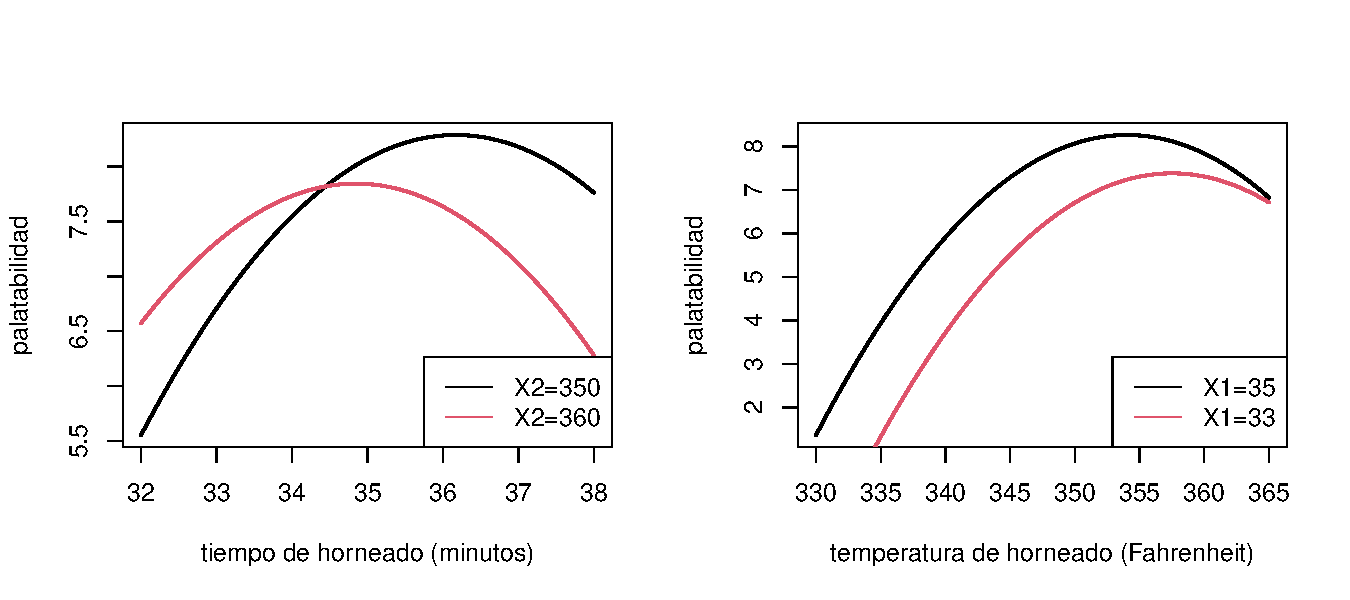
\includegraphics{MLG2_files/figure-latex/PredCakes-1} 

}

\caption{Datos de pasteles. Valor esperado de la palatabilidad para diferentes valores de tiempo y temperatura de horneado. }\label{fig:PredCakes}
\end{figure}

En la Figura \ref{fig:predCakes} (izquierda) vemos que, cuando la temperatura es de 350 grados Fahrenheit, el máximo de palatabilidad que se obtiene en un tiempo entre 36 y 37 minutos. Sin embargo, cuando la temperatura se incrementa a 360, la máxima palatibilidad que se puede lograr es menor. Además, se obtiene en un tiempo también menor. El efecto de la interacción también se puede observar en la Figura \ref{fig:predCakes2} (derecha), pero ahora fijando el tiempo de horneado y variando la temperatura. El gráfico de contornos (Figura \ref{fig:predCakes2}) muestra que la máxima palatabilidad se observa cuando la temperatura está alrededor de 355 y el tiempo de horneado está entre 35 y 36 minutos.

\begin{Shaded}
\begin{Highlighting}[]
\NormalTok{X1 }\OtherTok{=} \FunctionTok{seq}\NormalTok{(}\DecValTok{32}\NormalTok{, }\DecValTok{38}\NormalTok{, }\AttributeTok{length.out =} \DecValTok{50}\NormalTok{)}
\NormalTok{X2 }\OtherTok{=} \FunctionTok{seq}\NormalTok{(}\DecValTok{335}\NormalTok{, }\DecValTok{365}\NormalTok{, }\AttributeTok{length=} \DecValTok{50}\NormalTok{)}

\NormalTok{y }\OtherTok{\textless{}{-}} \FunctionTok{outer}\NormalTok{(}\AttributeTok{X=}\NormalTok{ X1, }\AttributeTok{Y =}\NormalTok{ X2, }\AttributeTok{FUN =} \ControlFlowTok{function}\NormalTok{(x, y) \{}
    \FunctionTok{predict}\NormalTok{(modc.cakes, }\AttributeTok{newdata =} \FunctionTok{data.frame}\NormalTok{(}\AttributeTok{X1c =}\NormalTok{ x}\SpecialCharTok{{-}}\FunctionTok{mean}\NormalTok{(cakes}\SpecialCharTok{$}\NormalTok{X1), }\AttributeTok{X2c =}\NormalTok{ y}\SpecialCharTok{{-}}\FunctionTok{mean}\NormalTok{(cakes}\SpecialCharTok{$}\NormalTok{X2)))}
\NormalTok{\})}

\FunctionTok{contour}\NormalTok{(X1, X2, y,}\AttributeTok{xlab=}\StringTok{\textquotesingle{}tiempo de horneado (minutos)\textquotesingle{}}\NormalTok{,}
        \AttributeTok{ylab=}\StringTok{\textquotesingle{}temperatura de horneado (Fahrenheit)\textquotesingle{}}\NormalTok{)}
\end{Highlighting}
\end{Shaded}

\begin{figure}

{\centering 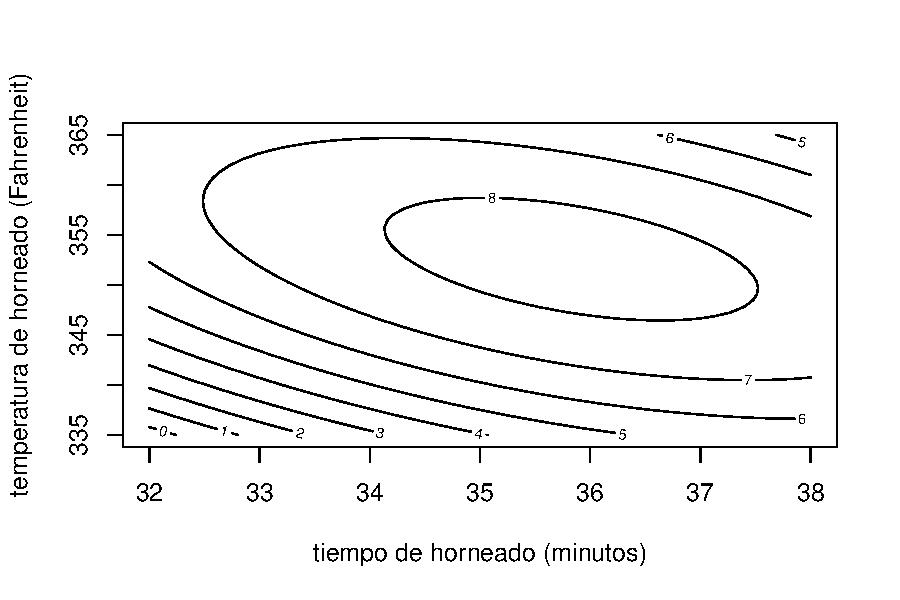
\includegraphics{MLG2_files/figure-latex/predCakes2-1} 

}

\caption{Datos de pasteles. Gráfica de contornos.}\label{fig:predCakes2}
\end{figure}

Para determinar en que combinación de tiempo (X1) y temperatura de horneado (X2) se obtiene la máxima palatabilidad. Por lo tanto, debemos resolver la siguiente ecuación:
\[
\frac{\partial E(Y)}{\partial \boldsymbol x}  = \frac{\partial}{\partial \boldsymbol x} \left( \beta_{0} + \beta_{1}x_{1} + \beta_{2}x_{2} + \beta_{3}x_{1}^2 + \beta_{4}x_{2}^{2} + \beta_{5}x_{1}x_{2} \right) = \boldsymbol 0,
\]
verificando que se obtiene un máximo.

Resolviendo la ecuación anterior, el máximo valor esperado de palatabilidad \((8.3)\) se obtiene en un tiempo de horneado de 35.8 minutos y a una temperatura de \ang{352.6}F. El intervalo del 95\% de confianza en este punto es: \((7.9, 8.7)\).

\hypertarget{datos-de-boston-1}{%
\subsubsection{Datos de Boston}\label{datos-de-boston-1}}

Para los datos de contaminación se puede proponer el siguiente modelo:
\[
\mbox{NOx}_{i}^{-1.5} = \beta_{0} + \beta_{1}\mbox{dis}_{i} + \beta_{2}\mbox{dis}_{i}^{2} + \beta_{3}\mbox{dis}_{i}^{3} + \varepsilon_{i}.
\]
La potencia en la variable respuesta se seleccionó usando el método de Box-Cox. El ajuste del modelo es el siguiente:

\begin{Shaded}
\begin{Highlighting}[]
\NormalTok{Boston}\SpecialCharTok{$}\NormalTok{disc }\OtherTok{=}\NormalTok{ Boston}\SpecialCharTok{$}\NormalTok{dis }\SpecialCharTok{{-}} \FunctionTok{mean}\NormalTok{(Boston}\SpecialCharTok{$}\NormalTok{dis)}
\NormalTok{mod3.Boston }\OtherTok{=} \FunctionTok{lm}\NormalTok{(}\FunctionTok{I}\NormalTok{(nox)}\SpecialCharTok{\^{}}\NormalTok{\{}\SpecialCharTok{{-}}\DecValTok{1}\NormalTok{\}}\SpecialCharTok{\textasciitilde{}}\NormalTok{disc}\SpecialCharTok{+}\FunctionTok{I}\NormalTok{(disc}\SpecialCharTok{\^{}}\DecValTok{2}\NormalTok{)}\SpecialCharTok{+}\FunctionTok{I}\NormalTok{(disc}\SpecialCharTok{\^{}}\DecValTok{3}\NormalTok{),}\AttributeTok{data=}\NormalTok{Boston)}
\FunctionTok{summary}\NormalTok{(mod3.Boston)}
\end{Highlighting}
\end{Shaded}

\begin{verbatim}
## 
## Call:
## lm(formula = I(nox)^{
##     -1
## } ~ disc + I(disc^2) + I(disc^3), data = Boston)
## 
## Residuals:
##      Min       1Q   Median       3Q      Max 
## -0.45677 -0.10233  0.00922  0.13091  0.32643 
## 
## Coefficients:
##               Estimate Std. Error t value Pr(>|t|)    
## (Intercept)  1.9785763  0.0121059 163.440  < 2e-16 ***
## disc         0.1788433  0.0051507  34.722  < 2e-16 ***
## I(disc^2)   -0.0257929  0.0029431  -8.764  < 2e-16 ***
## I(disc^3)    0.0013534  0.0004814   2.811  0.00513 ** 
## ---
## Signif. codes:  0 '***' 0.001 '**' 0.01 '*' 0.05 '.' 0.1 ' ' 1
## 
## Residual standard error: 0.173 on 502 degrees of freedom
## Multiple R-squared:  0.7765, Adjusted R-squared:  0.7752 
## F-statistic: 581.5 on 3 and 502 DF,  p-value: < 2.2e-16
\end{verbatim}

En la Figura @ref\{figPredBoston\} muestra el ajuste del modelo cúbico. Para hacer comparaciones, se muestra también el ajuste lineal y cuadrático. Se observa que el modelo cúbico presenta un buen ajuste. El modelo explica alrededor del \(78.3\)\% de la variabilidad de la concentración anual de óxido de nitrógeno. Con el modelo cuadrático, el coeficiente de determinación es de \(0.781\). Sin embargo, se puede observar que este ajuste es un poco deficiente cuando las distancias son muy grandes (mayores a 11).

\begin{figure}

{\centering 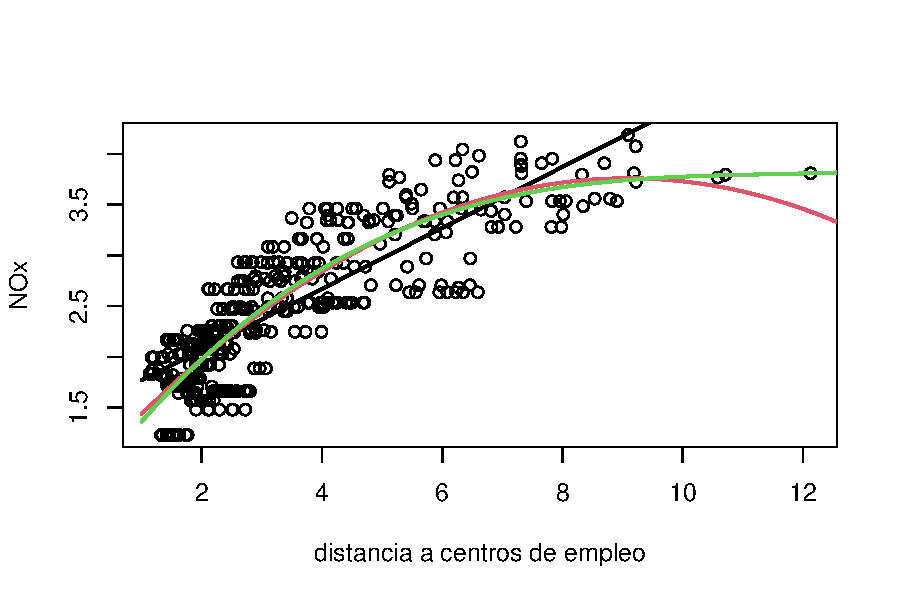
\includegraphics{MLG2_files/figure-latex/figPredBoston-1} 

}

\caption{Datos de Boston. Valor esperado de la concentración anual de óxido de nitrógeno (en partes por diez millones) en función de las distancias a cinco centros de empleo (media ponderada). Modelo lineal (negro), cuadrático (rojo) y cúbico (verde).}\label{fig:figPredBoston}
\end{figure}

\hypertarget{regresiuxf3n-por-segmentos}{%
\subsection{Regresión por segmentos}\label{regresiuxf3n-por-segmentos}}

El modelo por segmentos se puede expresar como:
\[
y_{i} = \beta_{0} + \beta_{1}x_{i} + \beta_{2}(x_{i}-t)^{0}_{+} +  \beta_{3}(x_{i}-t)^{1}_{+} + \varepsilon_{i}.
\]
donde:
\[
(x_{i}-t)_{+}^{r}  = \begin{cases}
0 & \mbox{ si } x_{i} + t \leq 0, \\
(x_{i}-t)^{r} & \mbox{ si } x_{i} + t > 0. \\
\end{cases}
\nonumber
\]
Por lo tanto, si \(x_{i} \leq t\), \(E(y_{i}| x_{i}) = \beta_{0} + \beta_{1}x_{i}\). Mientras que, si \(x_{i} > t\), tenemos que \(E(y_{i}| x_{i}) = (\beta_{0} + \beta_{2} - \beta_{1}t) + (\beta_{1} + \beta_{3})x_{i}\).

Este modelo esta representado graficamente en la Figura \ref{RegSegmentos}. Cuando \(\beta_2 \neq 0\), el modelo presenta una discontinuidad en \(t\). Mientras que, cuando \(\beta_2 = 0\), el modelo presenta un cambio de pendiente en el punto \(t\). Además, \(\beta_3\) indica el cambio de pendiente.

\begin{figure}

{\centering 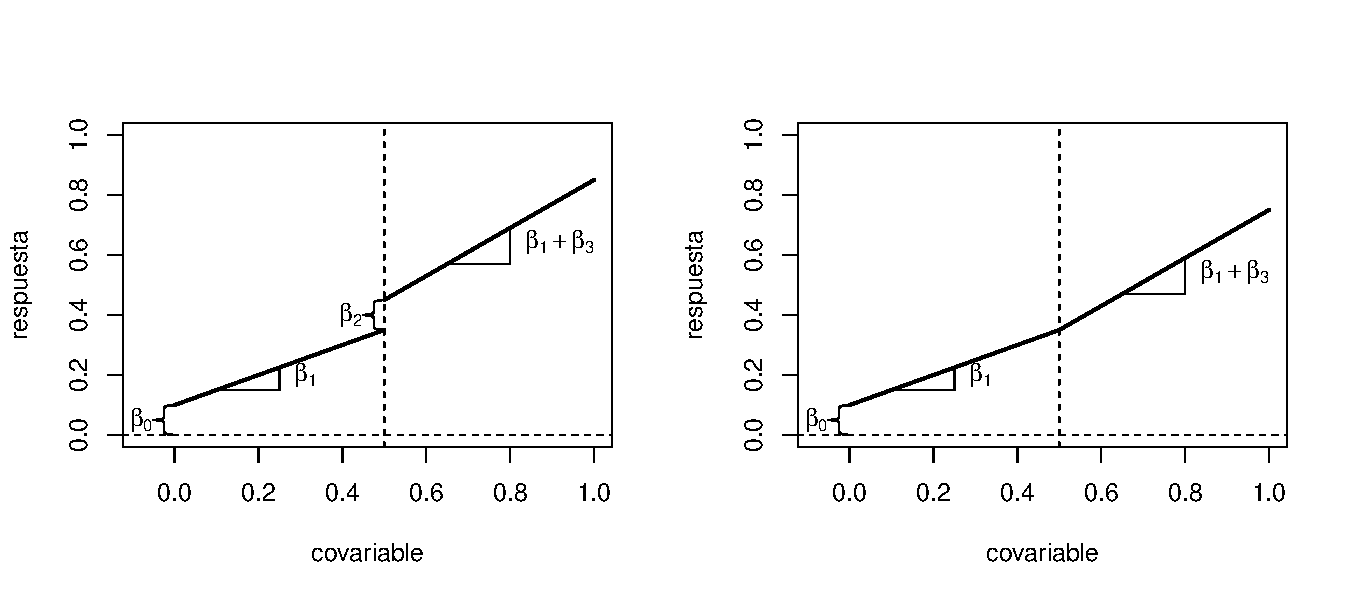
\includegraphics{MLG2_files/figure-latex/RegSegmentos-1} 

}

\caption{Modelo de regresión por segmentos. Modelo con discontinuidad en $t$ (izquierda). Modelo con cambio de pendiente en $t$ (derecha).}\label{fig:RegSegmentos}
\end{figure}

Aquí asumimos que \(t\) es conocido. Si este valor se asume como desconocido, debe estimarse a partir de los datos como un parámetro adicional. Sin embargo, se tendría que recurrir a un método estimación para modelos no-lineales.

\hypertarget{ejemplo}{%
\subsubsection{Ejemplo}\label{ejemplo}}

\begin{Shaded}
\begin{Highlighting}[]
\FunctionTok{library}\NormalTok{(MPV)}
\FunctionTok{data}\NormalTok{(p7}\FloatTok{.11}\NormalTok{)}
\FunctionTok{plot}\NormalTok{(p7}\FloatTok{.11}\NormalTok{,}\AttributeTok{ylab=}\StringTok{\textquotesingle{}costo de producción por unidad (USD)\textquotesingle{}}\NormalTok{,}\AttributeTok{xlab=}\StringTok{\textquotesingle{}Unidades por lote\textquotesingle{}}\NormalTok{)}
\end{Highlighting}
\end{Shaded}

\begin{figure}

{\centering 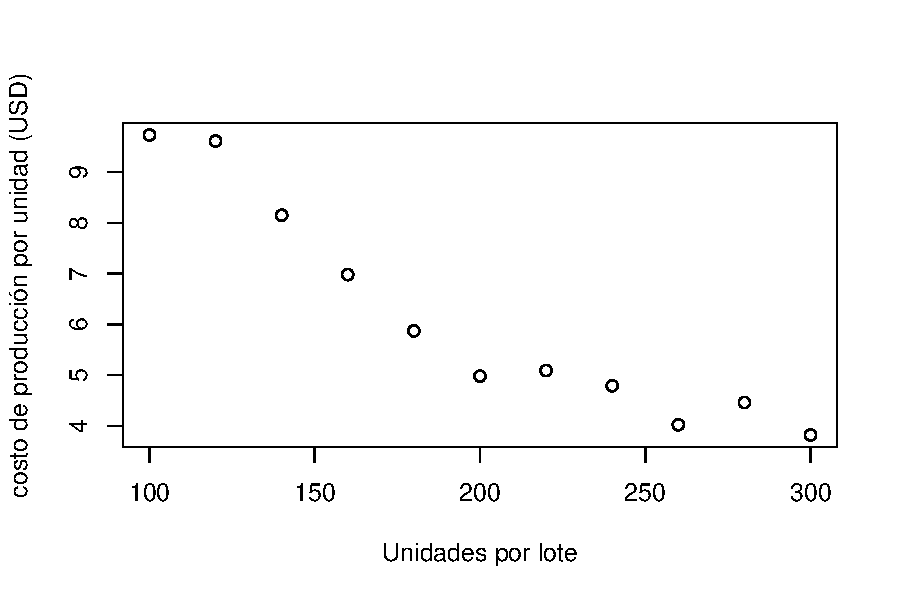
\includegraphics{MLG2_files/figure-latex/LotesFigure-1} 

}

\caption{Datos de costos por lote. Diagram de dispersión de el costo de producción promedio por unidad (USD) y el tamaño del lote (unidades).}\label{fig:LotesFigure}
\end{figure}

Considere la base de datos \texttt{p7.11} de la librería \texttt{MPV}. Aquí se quiere modelar la relación entre el costo de producción promedio por unidad (USD) y el tamaño del lote (unidades). Este relación se puede observar en la Figura \ref{fig:LotesFigure}. Se puede observar que la relación entre las variables es lineal. Sin embargo, se aprecia un posible cambio de pendiente en el punto \(x=200\). Por esta razón se propone el siguiente modelo:
\[
y_{i} = \beta_{0} + \beta_{1}x_{i} + \beta_{2}(x_{i}-200)_{+}^{1} + \varepsilon_{i}.
\]
Note que no se asume ninguna discontinuidad. El ajuste del modelo es:

\begin{Shaded}
\begin{Highlighting}[]
\NormalTok{p7}\FloatTok{.11}\SpecialCharTok{$}\NormalTok{x2 }\OtherTok{=}\NormalTok{ p7}\FloatTok{.11}\SpecialCharTok{$}\NormalTok{x }\SpecialCharTok{{-}} \DecValTok{200}
\NormalTok{p7}\FloatTok{.11}\SpecialCharTok{$}\NormalTok{x2[p7}\FloatTok{.11}\SpecialCharTok{$}\NormalTok{x }\SpecialCharTok{\textless{}} \DecValTok{200}\NormalTok{] }\OtherTok{=} \DecValTok{0}
\NormalTok{mod.lotes }\OtherTok{=} \FunctionTok{lm}\NormalTok{(y}\SpecialCharTok{\textasciitilde{}}\NormalTok{.,}\AttributeTok{data=}\NormalTok{p7}\FloatTok{.11}\NormalTok{)}
\FunctionTok{summary}\NormalTok{(mod.lotes)}
\end{Highlighting}
\end{Shaded}

\begin{verbatim}
## 
## Call:
## lm(formula = y ~ ., data = p7.11)
## 
## Residuals:
##      Min       1Q   Median       3Q      Max 
## -0.37596 -0.16641 -0.09677  0.20363  0.51734 
## 
## Coefficients:
##              Estimate Std. Error t value Pr(>|t|)    
## (Intercept) 15.116481   0.535383  28.235 2.67e-09 ***
## x           -0.050199   0.003332 -15.065 3.73e-07 ***
## x2           0.038852   0.005946   6.534 0.000181 ***
## ---
## Signif. codes:  0 '***' 0.001 '**' 0.01 '*' 0.05 '.' 0.1 ' ' 1
## 
## Residual standard error: 0.3157 on 8 degrees of freedom
## Multiple R-squared:  0.9829, Adjusted R-squared:  0.9787 
## F-statistic: 230.4 on 2 and 8 DF,  p-value: 8.474e-08
\end{verbatim}

A partir del ajuste podemos concluir que, por cada unidad que incrementa el lote, el costo de producción disminuye en \(0.05\)USD. Si embargo, si el tamaño del lote es mayor a \(200\), el costo de producción disminuye solamente \(0.01\)USD cuando el lote aumenta en un artículo. Gráficamente, el ajuste se puede observar en la Figura \ref{fig:LotesFigure2}.

\begin{Shaded}
\begin{Highlighting}[]
\NormalTok{b.lotes }\OtherTok{=}\NormalTok{ mod.lotes}\SpecialCharTok{$}\NormalTok{coefficients}
\FunctionTok{plot}\NormalTok{(p7}\FloatTok{.11}\SpecialCharTok{$}\NormalTok{x,p7}\FloatTok{.11}\SpecialCharTok{$}\NormalTok{y,}\AttributeTok{ylab=}\StringTok{\textquotesingle{}costo de producción por unidad (USD)\textquotesingle{}}\NormalTok{,}\AttributeTok{xlab=}\StringTok{\textquotesingle{}unidades por lote\textquotesingle{}}\NormalTok{)}
\NormalTok{x }\OtherTok{=} \FunctionTok{c}\NormalTok{(}\DecValTok{100}\NormalTok{,}\DecValTok{200}\NormalTok{)}
\FunctionTok{lines}\NormalTok{(x,b.lotes[}\DecValTok{1}\NormalTok{]}\SpecialCharTok{+}\NormalTok{x}\SpecialCharTok{*}\NormalTok{b.lotes[}\DecValTok{2}\NormalTok{],}\AttributeTok{lwd=}\DecValTok{2}\NormalTok{)}
\NormalTok{x }\OtherTok{=} \FunctionTok{c}\NormalTok{(}\DecValTok{200}\NormalTok{,}\DecValTok{300}\NormalTok{)}
\FunctionTok{lines}\NormalTok{(x,b.lotes[}\DecValTok{1}\NormalTok{]}\SpecialCharTok{{-}}\DecValTok{200}\SpecialCharTok{*}\NormalTok{b.lotes[}\DecValTok{3}\NormalTok{]}\SpecialCharTok{+}\NormalTok{x}\SpecialCharTok{*}\NormalTok{(b.lotes[}\DecValTok{2}\NormalTok{]}\SpecialCharTok{+}\NormalTok{b.lotes[}\DecValTok{3}\NormalTok{]),}\AttributeTok{lwd=}\DecValTok{2}\NormalTok{)}
\FunctionTok{abline}\NormalTok{(}\AttributeTok{v=}\DecValTok{200}\NormalTok{,}\AttributeTok{lty=}\DecValTok{2}\NormalTok{)}
\end{Highlighting}
\end{Shaded}

\begin{figure}

{\centering 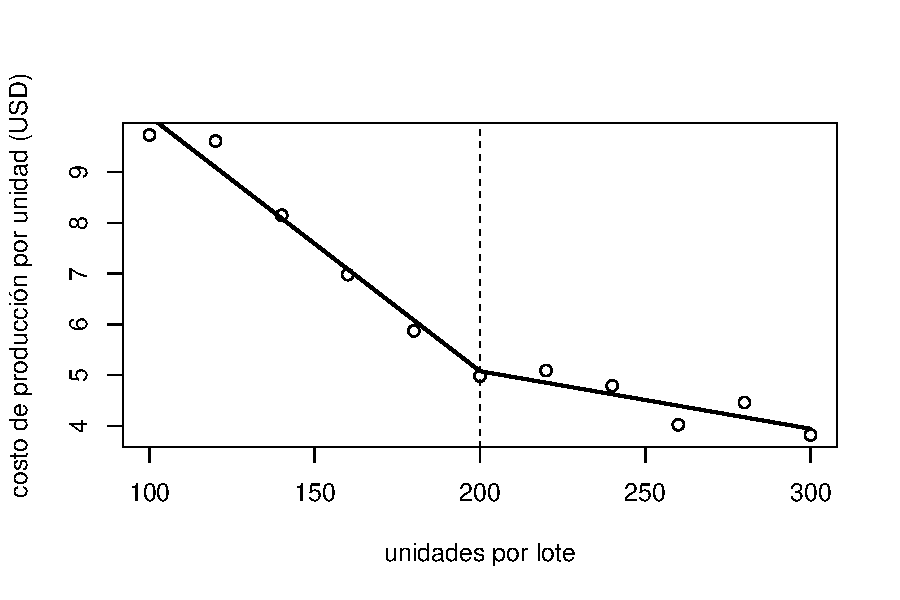
\includegraphics{MLG2_files/figure-latex/LotesFigure2-1} 

}

\caption{Datos de costos por lote. Diagram de dispersión de el costo de producción promedio por unidad (USD) y el tamaño del lote (unidades).}\label{fig:LotesFigure2}
\end{figure}

\hypertarget{multicolinealidad}{%
\section{Multicolinealidad}\label{multicolinealidad}}

\hypertarget{ejemplos-2}{%
\subsection{Ejemplos}\label{ejemplos-2}}

\hypertarget{cemento}{%
\subsubsection{Cemento}\label{cemento}}

Los datos \texttt{data(cement)} en la librería \texttt{MASS} corresponden a un experimento sobre calor emanado en el fraguado de diferentes combinaciones químicas de cemento. Se tiene una muestra de \(13\) fraguados de cemento Portlan. En cada muestra, se midió con precisión los porcentajes de los cuatro ingredientes químicos principales (covariables). Mientras el cemento fraguaba, también se midió la cantidad de calor desprendido (cals/gm, variable respuesta).

Los cuatro ingredientes químicos son:

\begin{itemize}
\tightlist
\item
  \textbf{\texttt{x1}} aluminato tricálcico (\%).
\item
  \textbf{\texttt{x2}} silicato tricálcico (\%).
\item
  \textbf{\texttt{x3}} tetra-aluminio ferrita de calcio (\%).
\item
  \textbf{\texttt{x4}} silicato dicálcico (\%).
\end{itemize}

En la Figura \ref{fig:CementFigure} podemos observar que hay relaciones lineales positivas entre la variable respuesta, y las covariables aluminato tricálcico y silicato tricálcico. Mientras que la relación con la variable silicato dicálcico es negativa. También podemos notar que hay una relación negativa fuerte en las covariables aluminato tricálcico y tetra-aluminio ferrita de calcio, y entre silicato tricálcico y silicato dicálcico.

\begin{Shaded}
\begin{Highlighting}[]
\FunctionTok{data}\NormalTok{(cement,}\AttributeTok{package =} \StringTok{\textquotesingle{}MASS\textquotesingle{}}\NormalTok{)}
\FunctionTok{plot}\NormalTok{(cement[,}\FunctionTok{c}\NormalTok{(}\DecValTok{5}\NormalTok{,}\DecValTok{1}\SpecialCharTok{:}\DecValTok{4}\NormalTok{)])}
\end{Highlighting}
\end{Shaded}

\begin{figure}

{\centering 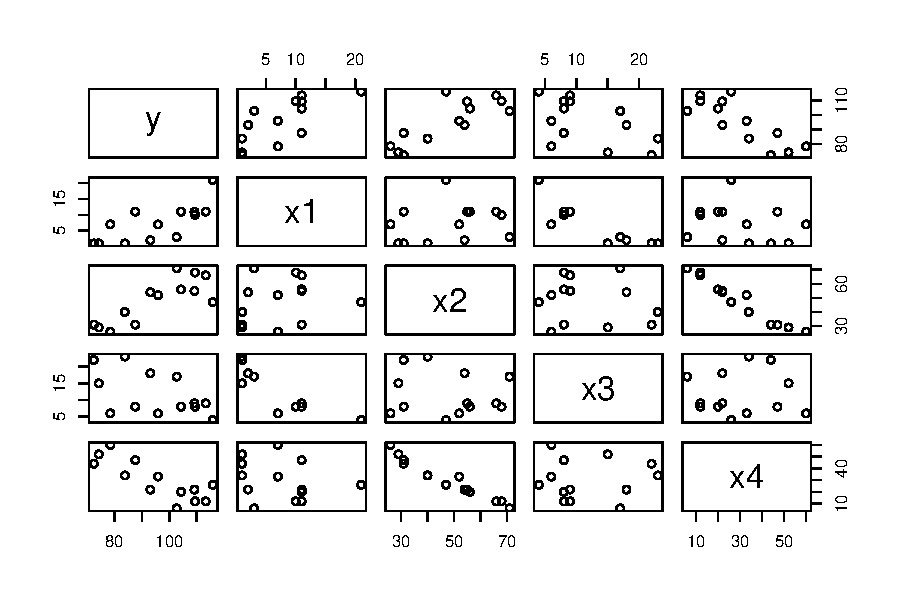
\includegraphics{MLG2_files/figure-latex/CementFigure-1} 

}

\caption{Datos de cemento. Diagrama de dispersión.}\label{fig:CementFigure}
\end{figure}

Para estos datos, se propone el siguiente modelo:
\[
y_{i} = \beta_{0} + x_{1i}\beta_{1} + x_{2i}\beta_{2} + x_{3i}\beta_{3} + x_{4i}\beta_{4} + \varepsilon_{i}.
\]
Los resultados del ajuste son:

\begin{Shaded}
\begin{Highlighting}[]
\NormalTok{mod.cement }\OtherTok{=} \FunctionTok{lm}\NormalTok{(y }\SpecialCharTok{\textasciitilde{}}\NormalTok{ x1}\SpecialCharTok{+}\NormalTok{x2}\SpecialCharTok{+}\NormalTok{x3}\SpecialCharTok{+}\NormalTok{x4,}\AttributeTok{data=}\NormalTok{cement)}
\FunctionTok{summary}\NormalTok{(mod.cement)}
\end{Highlighting}
\end{Shaded}

\begin{verbatim}
## 
## Call:
## lm(formula = y ~ x1 + x2 + x3 + x4, data = cement)
## 
## Residuals:
##     Min      1Q  Median      3Q     Max 
## -3.1750 -1.6709  0.2508  1.3783  3.9254 
## 
## Coefficients:
##             Estimate Std. Error t value Pr(>|t|)  
## (Intercept)  62.4054    70.0710   0.891   0.3991  
## x1            1.5511     0.7448   2.083   0.0708 .
## x2            0.5102     0.7238   0.705   0.5009  
## x3            0.1019     0.7547   0.135   0.8959  
## x4           -0.1441     0.7091  -0.203   0.8441  
## ---
## Signif. codes:  0 '***' 0.001 '**' 0.01 '*' 0.05 '.' 0.1 ' ' 1
## 
## Residual standard error: 2.446 on 8 degrees of freedom
## Multiple R-squared:  0.9824, Adjusted R-squared:  0.9736 
## F-statistic: 111.5 on 4 and 8 DF,  p-value: 4.756e-07
\end{verbatim}

Note que el ajuste es bueno, el \(98.2\)\% de la variabilidad de la cantidad de calor desprendido durante la fraguado es explicada por el modelo. Sin embargo, los resultados de las pruebas de hipótesis individuales sobre los coeficientes muestran que no son significantes.

\hypertarget{grasa-corporal}{%
\subsubsection{Grasa corporal}\label{grasa-corporal}}

Se tiene una muestra de \(20\) mujeres saludables con edades entre \(25\) y \(34\) años (\texttt{data(bodyfat)} en la librería \texttt{isdals}). La medición del porcentaje de grasa corporal es caro y engorroso, por lo tanto se quiere buscar un modelo que proporcione predicciones fiables. Como variables de este modelo se utiliza:

\begin{itemize}
\tightlist
\item
  \textbf{\texttt{Triceps}:} pliegue cutáneo del tríceps (cm).
\item
  \textbf{\texttt{Thigh}:} circunferencia del muslo (cm).
\item
  \textbf{\texttt{Midarm}:} circunferencia del brazo medio (cm).
\end{itemize}

La Figura @(fig:bodyfatFigure) muestra la relación entre variables. Podemos observar que hay una relación fuerte del \% de masa corporal con las covariables Triceps y Thigh. Además hay también una relación lineal fuerte entre esas dos covariables.

\begin{Shaded}
\begin{Highlighting}[]
\FunctionTok{library}\NormalTok{(isdals)}
\FunctionTok{data}\NormalTok{(bodyfat)}
\FunctionTok{plot}\NormalTok{(bodyfat)}
\end{Highlighting}
\end{Shaded}

\begin{figure}

{\centering 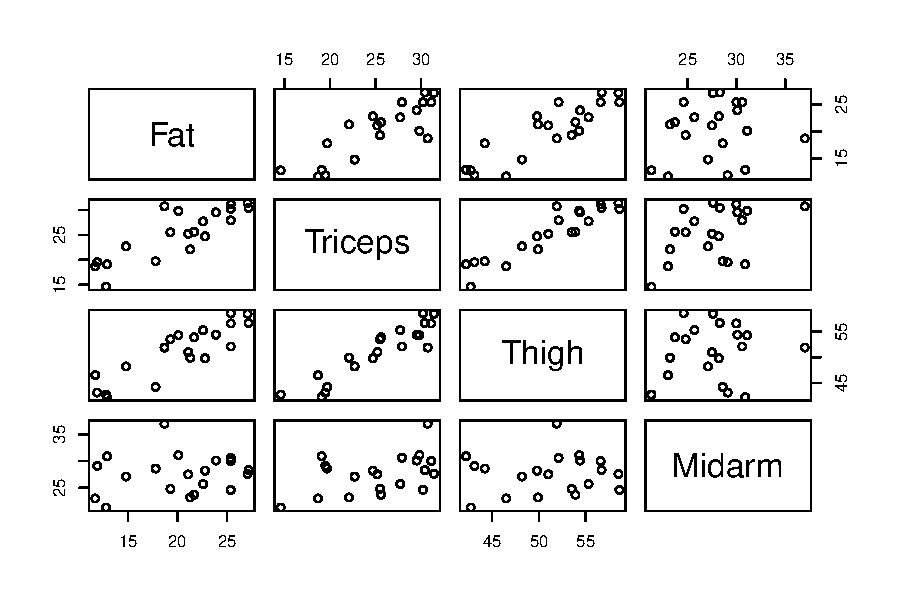
\includegraphics{MLG2_files/figure-latex/bodyfatFigure-1} 

}

\caption{Datos de grasa corporal. Diagrama de dispersión.}\label{fig:bodyfatFigure}
\end{figure}

El modelo propuesto es:
\[
\mbox{Fat}_{i} = \beta_{0} + \mbox{Triceps}_{i}\beta_{1} + \mbox{Thigh}_{i}\beta_{2} + \mbox{Midarm}_{i}\beta_{3} + \varepsilon_{i}.
\]
El ajuste del modelo es el siguiente:

\begin{Shaded}
\begin{Highlighting}[]
\NormalTok{mod.bodyfat }\OtherTok{=} \FunctionTok{lm}\NormalTok{(Fat }\SpecialCharTok{\textasciitilde{}}\NormalTok{ Triceps}\SpecialCharTok{+}\NormalTok{Thigh}\SpecialCharTok{+}\NormalTok{Midarm,}\AttributeTok{data=}\NormalTok{bodyfat)}
\FunctionTok{summary}\NormalTok{(mod.bodyfat)}
\end{Highlighting}
\end{Shaded}

\begin{verbatim}
## 
## Call:
## lm(formula = Fat ~ Triceps + Thigh + Midarm, data = bodyfat)
## 
## Residuals:
##     Min      1Q  Median      3Q     Max 
## -3.7263 -1.6111  0.3923  1.4656  4.1277 
## 
## Coefficients:
##             Estimate Std. Error t value Pr(>|t|)
## (Intercept)  117.085     99.782   1.173    0.258
## Triceps        4.334      3.016   1.437    0.170
## Thigh         -2.857      2.582  -1.106    0.285
## Midarm        -2.186      1.595  -1.370    0.190
## 
## Residual standard error: 2.48 on 16 degrees of freedom
## Multiple R-squared:  0.8014, Adjusted R-squared:  0.7641 
## F-statistic: 21.52 on 3 and 16 DF,  p-value: 7.343e-06
\end{verbatim}

Asi como en el caso anterior, observamos que el modelo explica gran parte de la variabilidad del \% de grasa corporal. Sin embargo, los valores \(p\) de las pruebas individuales sobre los coeficientes son altos.

\hypertarget{multicolinealidad-1}{%
\subsection{Multicolinealidad}\label{multicolinealidad-1}}

El estimador de \(\boldsymbol \beta\) es \(\widehat{\boldsymbol \beta}= (\boldsymbol X'\boldsymbol X)^{-1}\boldsymbol X'\boldsymbol y\). Además, \(V(\widehat{\boldsymbol \beta}) = \sigma^{2}(\boldsymbol X'\boldsymbol X)^{-1}\). Por lo tanto requiere que \(\boldsymbol X\) sea de rango completo. Es decir, que hayan columnas que sean linealmente dependientes. En algunos casos, las columnas de \(\boldsymbol X\) son casi linealmente dependientes o colineales,lo que lleva a que \(\boldsymbol X'\boldsymbol X\) se casi singular, lo que provoca problemas a la hora de hacer inferencias.

Sea \(\boldsymbol x_j\) la \(j\)-ésima columna de la matriz \(\boldsymbol X\), por lo tanto \(\boldsymbol X= (\boldsymbol 1,\boldsymbol x_{1},\ldots,\boldsymbol x_{p-1})\). Los vectores \(\boldsymbol x_{1},\boldsymbol x_{2},\ldots,\boldsymbol x_{p-1}\) son linealmente dependientes si hay conjunto de constantes \(a_{1},a_{2},\ldots, a_{p-1}\) no todas igual a cero, tal que:
\[
\sum_{j=1}^{p-1}a_{j}\boldsymbol x_{j} = c, \mbox{ donde }c\mbox{ es una constante.}
\]
Si esto se cumple para un subconjunto de \(\boldsymbol X\), el rango de la matriz \(\boldsymbol X'\boldsymbol X\) es menor que \(p\), y por lo tanto, \((\boldsymbol X'\boldsymbol X)^{-1}\) no existe.

Si la relación es aproximada \((\sum_{j=1}^{p-1}a_{j}\boldsymbol x_{j} \approx c)\), existe el problema de multicolinealidad.

Vamos a ilustrar el efecto de la multicolinealidad con un ejemplo sencillo considerando un modelo lineal con dos covariables:
\[
\boldsymbol y^{*} = \boldsymbol Z\boldsymbol \beta+ \boldsymbol \varepsilon,
\]
donde \(\boldsymbol Z\) es la matriz de covariables escaladas con longitud unitaria. Esto es:
\[
y_{i}^{*} = \frac{y_{i}-\bar{y}}{\sqrt{SST}}, \mbox{ y } z_{ij} = \frac{x_{ij} - \bar{x}_{j}}{\sqrt{s_{jj}}},
\]
donde \(s_{jj} = \sum_{i=1}^{n}(x_{ij}-\bar{x}_{j})^{2}\). De esta forma \(\boldsymbol Z'\boldsymbol Z\) es la matriz de correlación de las covariables,
\[
\boldsymbol Z'\boldsymbol Z= \begin{pmatrix}
1 & r_{12} \\ r_{12} & 1
\end{pmatrix},
\]
y \(\boldsymbol Z'\boldsymbol y\) es el vector de correlaciones entre \(y\) y las dos covariables:
\[
\boldsymbol Z'\boldsymbol y^{*} = \begin{pmatrix}
r_{y1} \\ r_{y2}
\end{pmatrix}.
\]
Por lo que el estimador por MCO de \(\boldsymbol b\) es:
\[
\widehat{\boldsymbol b}= \begin{pmatrix}
1 & r_{12} \\ r_{12} & 1
\end{pmatrix}^{-1}\begin{pmatrix}
r_{y1} \\ r_{y2}
\end{pmatrix} = \begin{pmatrix}
\frac{1}{1-r_{12}^{2}} & \frac{-r_{12}}{1-r_{12}^{2}} \\ \frac{-r_{12}}{1-r_{12}^{2}} & \frac{1}{1-r_{12}^{2}} \end{pmatrix} \begin{pmatrix}
r_{1y} \\ r_{2y}
\end{pmatrix}.
\]
Particularmente, tenemos:
\[
\widehat{b}_{1} = \frac{r_{1y}-r_{12}r_{2y}}{1-r_{12}^{2}} \mbox{ y } \widehat{b}_{2} = \frac{r_{2y}-r_{12}r_{1y}}{1-r_{12}^{2}}.
\]
Además, la matriz de varianzas-covarianzas de \(\widehat{\boldsymbol b}\) es:
\begin{equation}
V(\widehat{\boldsymbol b}) = \sigma^{2} \begin{pmatrix}
\frac{1}{1-r_{12}^{2}} & \frac{-r_{12}}{1-r_{12}^{2}} \\ \frac{-r_{12}}{1-r_{12}^{2}} & \frac{1}{1-r_{12}^{2}} \end{pmatrix}.
\label{eq:varbb}
\end{equation}
En \eqref{eq:varbb} podemos observar que la varianza de los coeficientes \(\widehat{\boldsymbol b}\) tienden a infinito cuando \(|r_{12}|\rightarrow 1\). Mientras que se hace mínima cuando las covariables están incorrelacionadas \((r_{12}=0)\). Es decir, una fuerte correlación entre \(x_1\) y \(x_2\) da como resultado grandes varianzas y covarianzas para \(\widehat{\boldsymbol b}\).

Por esta razón es preferible tener covariables que sean ortogonales. Puesto que así se garantiza la menor varianza para \(\widehat{\boldsymbol \beta}\). Sin embargo, las covariables son díficiles de controlar en estudios observacionales.

Ahora consideremos un modelo con \(p-1\) covariables,
\[
y_{i}^{*} = b_{1}z_{i1} + b_{2}z_{i2} + \ldots + b_{p-1}z_{i,p-1} + \varepsilon_{i}.
\]
Las ecuaciones normales son:
\[
\begin{pmatrix}
1 & r_{12} & r_{13} & \ldots & r_{1,p-1}  \\ r_{12} & 1 & r_{23} & \ldots & r_{2,p-1} \\
\vdots & \vdots & \vdots & \ddots & \vdots \\
r_{1,p-1} & r_{2,p-1} & r_{3,p-1} & \ldots & 1
\end{pmatrix} \begin{pmatrix}
b_{1} \\ b_{2} \\ \vdots \\ b_{p-1}
\end{pmatrix} = \begin{pmatrix}
r_{y1} \\ r_{y2} \\ \vdots \\ r_{y,p-1}
\end{pmatrix}.
\]
Por lo que el estimador de \(\boldsymbol b\) es:
\[
\widehat{\boldsymbol b}= \boldsymbol R^{-1}\boldsymbol Z'\boldsymbol y^{*}, \mbox{donde }\boldsymbol R= \boldsymbol Z'\boldsymbol Z.
\]
Se puede demostrar que los elementos de la diagonal de la matriz \(\boldsymbol R^{-1}\) son:
\[
\{\boldsymbol R^{-1}\}_{jj} = \frac{1}{1-R^{2}_{j}}, j=1,\ldots,p-1,
\]
donde \(R^{2}_{j}\) es el coeficiente de determinación de la regresión de \(z_{j}\) en función de las \((p-2)\) covariables restantes. Es decir, coeficiente de determinacón del siguiente ajuste:
\[
z_{ij} = z_{i1}\alpha_1 + z_{i2}\alpha_2 + \ldots + z_{i,j-1}\alpha_{j-1} + z_{i,j+1}\alpha_{j+1} + \ldots + z_{i,p-1}\alpha_{p-1} + \varepsilon_i.
\]

Por lo que la varianza del estimador de \(\boldsymbol b\) es:
\[
V(\widehat{b}_{j}) = \frac{\sigma^{2}}{1-R^{2}_{j}}.
\]
Por lo que, si \(z_j\) se puede expresar como una combinación lineal aproximada de las demás covariables, la varianza del estimador de \(b_j\) Si \(R^{2}_{j} \rightarrow 1\), entonces \(V(\widehat{b}_{j})\rightarrow \infty\).

La multicolinealidad también produce que los estimadores \(\widehat{b}_{j}\), para \(j=1,\ldots,p-1\), sean muy grandes en valor absoluto. Considere:
\[
L_{1}^{2} = (\widehat{\boldsymbol b}- \boldsymbol b)'(\widehat{\boldsymbol b}- \boldsymbol b) = \sum_{j=1}^{p}(\widehat{b}_{j}-b_{j})^{2}.
\]
El valor esperado de \(L_{1}^{2}\) es:
\[
E(L_{1}^{2}) = \sum_{j=1}^{p-1}E(\widehat{b}_{j}-b_{j})^{2} = \sum_{j=1}^{p-1}\sigma^{2}\mbox{tr}\boldsymbol R^{-1}
\]
Dado que la traza de una matriz es igual a la suma de sus valores propios, tenemos que:
\[
E(L_{1}^{2}) = \sigma^{2}\sum_{j=1}^{p-1}1/\lambda_{j},
\]
donde \(\lambda_{j} > 0\), para \(j=1,\ldots,p-1\), son los valores propios de \(\boldsymbol R\). Por lo tanto, si \(\boldsymbol R\) está mal condicionada debido a la multicolinealidad, al menos un \(\lambda_{j}\) será muy pequeño.

Cabe notar que, la multicolinealidad no viola ningún supuesto sobre los errores. Por lo tanto los estimadores por MCO siguen siendo BLUE. Pero, en presencia de multicolinealidad:

\begin{itemize}
\item
  Las varianzas de los coeficientes \((\widehat{\beta}_{j})\) se incrementan. Lo que reduce los valores \(t\) asociados.
\item
  Los \(\widehat{\beta}_{j}\) son sensibles a las especificaciones. Estos pueden cambiar drásticamente cuando se agregan o eliminan covariables.
\item
  El ajuste general del modelo, y por lo tanto los pronósticos y las predicciones, no se verá afectado en gran medida. Pero los intervalos de confianza que se calculen pueden ser muy amplios.
\end{itemize}

\hypertarget{causas-de-la-multicolinealidad}{%
\subsubsection{Causas de la multicolinealidad}\label{causas-de-la-multicolinealidad}}

La multicolinealidad se puede deber a múltiples razones, entre las que están:

\begin{itemize}
\item
  Con frecuencia se presentan problemas donde intervienen procesos de producción o químicos, donde los regresores son los componentes de un producto y ésos suman una constante.
\item
  Variables que son componentes de un sistema pueden mostrar dependencias casi lineales debido a las limitaciones biológicas, físicas o químicas del sistema.
\item
  Variables que tienen una tendencia común y evolucionan de forma muy parecida en el tiempo.
\item
  Inclusión de variables irrelevantes en el modelo. La información que contienen estas variables ya estarían incluidas en otras y no aportan a la explicación de la variabilidad de la variable respuesta.
\end{itemize}

Por ejemplo, en los datos del cemento, tenemos que el problema de multicolinealidad se presenta porque:
\[
x_{i1} + x_{i2} + x_{i3} + x_{i4} \approx \mbox{constante}.   
\]
En los datos de grasa corporal, el problema es causado por la alta correlación entre el pliegue cutáneo del triceps \((X_{1})\) y la circunferencia del muslo \((X_{2})\).

\hypertarget{detecciuxf3n-de-multicolinealidad}{%
\subsection{Detección de multicolinealidad}\label{detecciuxf3n-de-multicolinealidad}}

Dado que la multicolinealidad provoca una inflación de la varianza, un indicio de este problema esta en que aunque el modelo presenta un buen ajuste (un \(R^2\) por ejemplo), las estimaciones de coeficientes asociados a covariables releventas tienen valores \(t\) pequeños. Además, al eliminar covariables, las estimacioes cambian considerablemente.

Los métodos mas usados para detectar multicolinealidad son:

\begin{itemize}
\item
  la matriz de correlación de las covariables.
\item
  los factores de inflación de varianza.
\item
  los índices de condiciones de \(\boldsymbol R\) o \(\boldsymbol Z\).
\end{itemize}

\hypertarget{factores-de-inflaciuxf3n-de-varianza}{%
\subsubsection{Factores de inflación de varianza}\label{factores-de-inflaciuxf3n-de-varianza}}

Dado que \(V(\widehat{\boldsymbol b}) = \sigma^2\boldsymbol R^{-1}\), la diagonal de \(\boldsymbol R^{-1}\) es un buen indicador de multicolinealidad:
\[
\{\boldsymbol R^{-1}\}_{jj} = (1-R_{j}^{2})^{-1},
\]
donde \(R_{j}^{2}\) es el coeficiente de determinación de ajustar un modelo de \(x_{j}\) en función de las demás covariables. Si \(x_{j}\) es casi ortogonal a las demás covariables, \(R^{2}_{j}\) es pequeño, y por lo tanto, \(\{\boldsymbol R^{-1}\}_{jj}\) cercano a \(1\). Mientras que, si \(x_{j}\) es casi linealmente dependiente a las demás covariables, entonces \(R^{2}_{j}\) es cercano a \(1\) y \(\{\boldsymbol R^{-1}\}_{jj}\) grande.

Es decir, \(\{\boldsymbol R^{-1}\}_{jj}\) puede ser visto como un factor de cuanto se incrementa \(V(\widehat{b}_{j})\) debido a la colinealidad entre las covariables. De aquí el nombre de factor de inflación de varianza (VIF). Generalmente, uno o mas valores grandes de VIF (\(5\) o \(10\)) es un indicador de problemas de multicolinealidad.

\hypertarget{valores-propios-de-boldsymbol-zboldsymbol-z}{%
\subsubsection{\texorpdfstring{Valores propios de \(\boldsymbol Z'\boldsymbol Z\)}{Valores propios de \textbackslash boldsymbol Z'\textbackslash boldsymbol Z}}\label{valores-propios-de-boldsymbol-zboldsymbol-z}}

Dado que \(\boldsymbol R= \boldsymbol Z'\boldsymbol Z\) es una matriz simétrica y positiva semi-definida, entonces se puede descomponer:
\[
\boldsymbol R= \boldsymbol T\boldsymbol \Lambda\boldsymbol T',
\]
donde \(\boldsymbol T= (\boldsymbol t_{1},\ldots,\boldsymbol t_{k})\) es una matriz ortogonal de vectores propios, y \(\boldsymbol \Lambda\) una matriz diagonal con los valores propios \(\lambda_{j}\), para \(j=1,\ldots,p-1\), en la diagonal principal. Por lo tanto,
\[
V(\widehat{\boldsymbol \beta}) = \sigma^{2}\boldsymbol T\boldsymbol \Lambda^{-1}\boldsymbol T'.
\]
Entonces,
\[
V(\widehat{b}_{j}) = \sigma^{2}\sum_{k=1}^{p-1}\frac{t_{jk}^{2}}{\lambda_{k}}.
\]
De la expresión anterior,
\[
VIF_{j} = \sum_{j=1}^{p-1}\frac{t_{ij}^{2}}{\lambda_{j}},
\]
Por lo tanto, uno o más valores propios pequeños pueden inflar la varianza de \(\widehat{b}_{j}\). De aquí salen los indicadores llamados índices de condición y número de condición.

El índice de condición está definido como:
\[
\eta_{j} = \frac{\lambda_{\mbox{max}}}{\lambda_{j}}.
\]
El número de condición está definido como el máximo índice de condición. Un número de condición mayor de 100 es un indicador de multicolinealidad.

\hypertarget{valores-singulares-de-boldsymbol-z}{%
\subsubsection{\texorpdfstring{Valores singulares de \(\boldsymbol Z\)}{Valores singulares de \textbackslash boldsymbol Z}}\label{valores-singulares-de-boldsymbol-z}}

El número de condición también se puede calcular a partir de la descomposición en valores singulares (SVD) de la matriz de covariables \(\boldsymbol Z\). Esto es:
\[
\boldsymbol Z=\boldsymbol U\boldsymbol D\boldsymbol T',
\]
donde \(\boldsymbol U\) y \(\boldsymbol T\) son matrices \(n\times (p-1)\) y \((p-1)\times (p-1)\), respectivamente, \(\boldsymbol U\boldsymbol U= \boldsymbol I\) y \(\boldsymbol T'\boldsymbol T= \boldsymbol I\), y \(\boldsymbol D\) es una matriz diagonal con elementos \(\mu_{j}\), \(j=1,\ldots,p-1\), llamados valores singulares.

Hay una relación entre los valoes singulares de \(\boldsymbol Z\) y los valores propios de \(\boldsymbol Z'\boldsymbol Z\):
\[
\boldsymbol Z'\boldsymbol Z= (\boldsymbol U\boldsymbol D\boldsymbol T')'\boldsymbol U\boldsymbol D\boldsymbol T' = \boldsymbol T\boldsymbol D^2\boldsymbol T' = \boldsymbol T\boldsymbol \Lambda\boldsymbol T'.
\]
El índice de condición de \(\boldsymbol Z\) está definido como:
\[
\kappa_{j} = \frac{\mu_{\mbox{max}}}{\mu_{j}}.
\]
El número de condición de \(\boldsymbol Z\) está definido como el máximo \(\kappa_{j}\). Un número de condición mayor de 10,15 o 30 es un indicador de problemas de multicolinealidad.

Note que \(\kappa_{j} = \sqrt{\eta_{j}}\). Por lo que el punto de corte de \(10\) para el número de condición de \(\boldsymbol Z\) es equivalente al número de condición de \(100\) para el número de condición de \(\boldsymbol Z'\boldsymbol Z\).

\hypertarget{proporciones-de-descomposiciuxf3n-de-varianza}{%
\subsubsection{Proporciones de descomposición de varianza}\label{proporciones-de-descomposiciuxf3n-de-varianza}}

Hay una relación entre el VIF, los valores propios y los valores singulares. Esta es:
\[
VIF_{j} = \sum_{j=1}^{p-1}\frac{t_{ij}^{2}}{\lambda_{j}} = \sum_{j=1}^{p-1}\frac{t_{ij}^{2}}{\mu_{j}^2}.
\]
De aquí salen los indicadores llamados proporciones de descomposición de varianza. Estos se calculan de la siguiente forma:
\[
\pi_{ij} = \frac{t_{ij}^2 / \mu_{i}^2 }{VIF_{j}}, j = 1,\ldots, p-1.
\]
Si se agrupan los \(\pi_{ij}\) en una matriz \((p-1) \times (p-1)\) \(\boldsymbol \pi\), la columna \(j\) son proporciones de la varianza de \(\widehat{\boldsymbol b}\). Valores \(\pi_{ij}\) mayores de 0.5 indican problemas de multicolinealidad.

\hypertarget{datos-de-cemento}{%
\subsection{Datos de cemento}\label{datos-de-cemento}}

Los VIF para el modelo ajustado para los datos de cemento son los siguientes:

\begin{Shaded}
\begin{Highlighting}[]
\NormalTok{car}\SpecialCharTok{::}\FunctionTok{vif}\NormalTok{(mod.cement)}
\end{Highlighting}
\end{Shaded}

\begin{verbatim}
##        x1        x2        x3        x4 
##  38.49621 254.42317  46.86839 282.51286
\end{verbatim}

Aquí vemos que todos los VIFs son muy altos, mostrando que hay problemas graves de multicolinealidad.

Para calcular los índices de condición (a partir de los valores singulares de \(\boldsymbol Z\)) y las proporciones de descomposición de varianza se utiliza la función \texttt{colldiag()} de la librería \texttt{perturb}:

\begin{Shaded}
\begin{Highlighting}[]
\FunctionTok{library}\NormalTok{(perturb)}
\FunctionTok{colldiag}\NormalTok{(mod.cement,}\AttributeTok{scale =} \ConstantTok{TRUE}\NormalTok{,}\AttributeTok{center =} \ConstantTok{TRUE}\NormalTok{,}\AttributeTok{add.intercept =} \ConstantTok{FALSE}\NormalTok{)}
\end{Highlighting}
\end{Shaded}

\begin{verbatim}
## Condition
## Index    Variance Decomposition Proportions
##           x1    x2    x3    x4   
## 1   1.000 0.003 0.001 0.001 0.000
## 2   1.191 0.004 0.000 0.005 0.000
## 3   3.461 0.064 0.002 0.046 0.001
## 4  37.106 0.930 0.997 0.947 0.998
\end{verbatim}

El número de condición \((37.106)\) es muy alto reafirmando el problema de multicolinealidad. Además, también se puede observar que varias de las proporciones de descomposición de varianza son mayores de \(0.5\).

\hypertarget{datos-de-grasa-corporal}{%
\subsection{Datos de grasa corporal}\label{datos-de-grasa-corporal}}

Para el modelo ajustado a losdatos de grasa corporal, los VIFs son:

\begin{Shaded}
\begin{Highlighting}[]
\NormalTok{car}\SpecialCharTok{::}\FunctionTok{vif}\NormalTok{(mod.bodyfat)}
\end{Highlighting}
\end{Shaded}

\begin{verbatim}
##  Triceps    Thigh   Midarm 
## 708.8429 564.3434 104.6060
\end{verbatim}

Además, los índices de condición y las proporciones de descomposición de varianza son:

\begin{Shaded}
\begin{Highlighting}[]
\FunctionTok{library}\NormalTok{(perturb)}
\FunctionTok{colldiag}\NormalTok{(mod.bodyfat,}\AttributeTok{scale =} \ConstantTok{TRUE}\NormalTok{,}\AttributeTok{center =} \ConstantTok{TRUE}\NormalTok{,}\AttributeTok{add.intercept =} \ConstantTok{FALSE}\NormalTok{)}
\end{Highlighting}
\end{Shaded}

\begin{verbatim}
## Condition
## Index    Variance Decomposition Proportions
##           Triceps Thigh Midarm
## 1   1.000 0.000   0.000 0.001 
## 2   1.488 0.000   0.000 0.008 
## 3  53.329 1.000   0.999 0.991
\end{verbatim}

Todos estos indicadores muestran que hay problemas de multicolinealidad.

\hypertarget{soluciuxf3n-al-problema-de-multicolinealidad}{%
\subsection{Solución al problema de multicolinealidad}\label{soluciuxf3n-al-problema-de-multicolinealidad}}

Una forma sencilla de resolver los problemas de multicolinealidad son:

\begin{itemize}
\item
  la recolección de datos adicionales: si se tiene control sobre las covariables, es posible tomar más observaciones para romper con la casi dependencia en \(\boldsymbol X\). Pero esto en muchas casos es díficl por la naturaleza de las covariables. Por ejemplo, sería imposible buscar personas con circunferencia del muslo grande y pliegue cutáneo del tríceps bajo (o viceversa).
\item
  la re-especificación del modelo: se pueden eliminar del modelo las covariables que me generan el problema de multicolinealidad y que pueden tener poco aporte explicativo dentro del modelo.
\end{itemize}

Por ejemplo, en los datos de la grasa corporal podemos eliminar la variable asociada al muslo (o al tríceps, pues ambas proporcionan la misma información). Si quitamos esta covariable:

\begin{Shaded}
\begin{Highlighting}[]
\NormalTok{mod.bodyfat0 }\OtherTok{=} \FunctionTok{lm}\NormalTok{(Fat }\SpecialCharTok{\textasciitilde{}}\NormalTok{ Triceps}\SpecialCharTok{+}\NormalTok{Midarm,}\AttributeTok{data=}\NormalTok{bodyfat)}
\NormalTok{car}\SpecialCharTok{::}\FunctionTok{vif}\NormalTok{(mod.bodyfat0)}
\end{Highlighting}
\end{Shaded}

\begin{verbatim}
##  Triceps   Midarm 
## 1.265118 1.265118
\end{verbatim}

los VIFs disminuyen considerablemente. Además, no hay una reducción notable del \(R^2\). Con las tres covariables temenos que \(R^{2}=0.801\). Mientras que al remover \texttt{Thigh}, tenemos que \(R^{2} = 0.786\)

Considerando que el estimador por MCO es el mejor estimador lineal insesgado de \(\boldsymbol \beta\), podemos relajar la condición de insesgamiento y buscar estimadores que aunque sean sesgados tengan menor varianza que los estimadores por MCO.

Dos de estas alternativas son:

\begin{itemize}
\item
  Estimador de ridge.
\item
  Estimadores por componentes principales.
\end{itemize}

\hypertarget{estimador-de-ridge}{%
\subsection{Estimador de ridge}\label{estimador-de-ridge}}

El estimador de ridge tiene como objetivo minimizar la siguiente suma de cuadrados penalizada:
\begin{equation}
\begin{split}
S_{R}(\boldsymbol b) &= \sum_{i=1}^{n}(y_{i} - \boldsymbol z_{i}'\boldsymbol b)^{2} + k \sum_{j=1}^{p-1}\boldsymbol b_{j}^2 \\
&= (\boldsymbol y- \boldsymbol Z\boldsymbol b)'(\boldsymbol y- \boldsymbol Z\boldsymbol b) + k ||\boldsymbol b||_{2}^{2},
\end{split}
\nonumber
\end{equation}
con \(k \geq 0\) (el cual es seleccionado por el investigador). Lo que lleva a las siguientes ecuaciones normales:
\[
(\boldsymbol R+ k \boldsymbol I)\widehat{\boldsymbol b}_{R} = \boldsymbol Z'\boldsymbol y.
\]
La solución de las ecuaciones normales lleva al estimador ridge:
\[
\widehat{\boldsymbol b}_{R} = (\boldsymbol R+ k \boldsymbol I)^{-1}\boldsymbol Z'\boldsymbol y.
\]
Note que, incluso si \(\boldsymbol R\) es no es invertible, un \(k > 0\) resuelve el problema. Además, la solución depende de \(k\) (por cada \(k\), hay una estimación diferente).

\(k\) es un parámetro de contracción:

\begin{itemize}
\tightlist
\item
  si \(k \rightarrow 0\), encontramos que \(\widehat{\boldsymbol b}_{R} \rightarrow \widehat{\boldsymbol b}\).
\item
  si \(k \rightarrow \infty\), encontramos que \(\widehat{\boldsymbol b}_{R} \rightarrow \boldsymbol 0\) (excepto el intercepto).
\end{itemize}

Ahora veamos las propiedades del estimador de ridge. El valor esperado de \(\widehat{\boldsymbol b}_{R}\) es:
\[
E(\widehat{\boldsymbol b}_{R}) = (\boldsymbol R+ k \boldsymbol I)^{-1}\boldsymbol R\boldsymbol b.
\]
De aquí vemos que \(\widehat{\boldsymbol b}_{R}\) es sesgado, y aumenta con \(k\) (por lo que este parámetro también es llamado de sesgo). La varianza de \(\widehat{\boldsymbol b}_{R}\) es:
\[
V(\widehat{\boldsymbol b}_{R}) = \sigma^{2}(\boldsymbol R+ k \boldsymbol I)^{-1}\boldsymbol R(\boldsymbol R+ k \boldsymbol I)^{-1}.
\]
A partir de las cantidades anteriores se puede determinar el error cuadrático medio (ECM) de \(\widehat{\boldsymbol b}_{R}\):
\begin{equation}
\begin{split}
\mbox{ECM}(\widehat{\boldsymbol b}_{R}) &= \sigma^{2}\mbox{tr}[(\boldsymbol R+ k\boldsymbol I)^{-1}\boldsymbol R(\boldsymbol R+ k\boldsymbol I)^{-1}] + k^{2}\boldsymbol b'(\boldsymbol R+ k\boldsymbol I)^{-2}\boldsymbol b\\
&=\sigma^{2}\sum_{i=1}^{p-1}\frac{\lambda_{j}}{(\lambda_{j}+ k)^2} + k^{2} \boldsymbol b'(\boldsymbol R+ k\boldsymbol I)^{-2}\boldsymbol b,
\end{split}
\nonumber
\end{equation}
donde \(\lambda_{1},\ldots,\lambda_{k}\) son los valores propios de \(\boldsymbol R\).

Finalmente, la suma de cuadrados de los residuos usando \(\widehat{\boldsymbol b}_{R}\) es:
\[
SS_{\mbox{res}}= (\boldsymbol y- \boldsymbol X\widehat{\boldsymbol b})'(\boldsymbol y- \boldsymbol X\widehat{\boldsymbol b}) + (\widehat{\boldsymbol b}_{R}-\widehat{\boldsymbol b})'\boldsymbol R(\widehat{\boldsymbol b}_{R}-\widehat{\boldsymbol b}).
\]
A partir de estos resultados, vemos que: (1) Si \(k\) crece, disminuye la varianza, pero aumenta el sesgo. (2) Si \(k\) disminuye, aumenta la varianza, pero disminuye el sesgo. (3) el estimador ridge proporciona un \(R^{2}\) mas pequeño que el estimador por MCO. Además, \(R^2\) disminuye con \(k\). Sin embargo, la regresión ridge proporciona estimaciones de \(\boldsymbol b\) más estables.

La idea de la regresión de ridge es encontrar un valor de \(k\) tal que \(\mbox{ECM}(\widehat{\boldsymbol b}_{R}) < V(\widehat{\boldsymbol b})\). En la Figura \ref{fig:ECMrepresentacion} podemos ver la representación del ECM del estimador de ridge. Aquí vemos que a medida que aumenta \(k\), el sesgo incrementa y la varianza disminuye. También, hay una región de \(k\) donde se puede obtener un ECM del estimador de ridge menor que el que se obtiene por medio de MCO. La idea es encontrar el valor de \(k\) que minimiza el ECM, o por lo menos algún valor en la región donde \(\mbox{ECM}(\widehat{\boldsymbol b}_{R}) < V(\widehat{\boldsymbol b})\).

\begin{Shaded}
\begin{Highlighting}[]
\NormalTok{x}\OtherTok{=} \FunctionTok{seq}\NormalTok{(}\AttributeTok{from=}\DecValTok{0}\NormalTok{,}\AttributeTok{to=}\FloatTok{0.3}\NormalTok{,}\AttributeTok{length.out =} \DecValTok{100}\NormalTok{)}
\NormalTok{sesgo }\OtherTok{=} \FloatTok{0.25}\SpecialCharTok{/}\NormalTok{(}\DecValTok{1}\SpecialCharTok{+}\FunctionTok{exp}\NormalTok{(}\SpecialCharTok{{-}}\DecValTok{20}\SpecialCharTok{*}\NormalTok{(x}\FloatTok{{-}0.001}\NormalTok{)))}
\NormalTok{sesgo }\OtherTok{=}\NormalTok{ sesgo }\SpecialCharTok{{-}} \FunctionTok{min}\NormalTok{(sesgo) }
\NormalTok{vari }\OtherTok{=} \FloatTok{0.06}\SpecialCharTok{*}\FunctionTok{exp}\NormalTok{(}\SpecialCharTok{{-}}\DecValTok{70}\SpecialCharTok{*}\NormalTok{x)}\SpecialCharTok{+} \FloatTok{0.0025}
\NormalTok{ecm }\OtherTok{=}\NormalTok{sesgo}\SpecialCharTok{+}\NormalTok{vari}
\FunctionTok{plot}\NormalTok{(x,sesgo,}\AttributeTok{type =} \StringTok{\textquotesingle{}l\textquotesingle{}}\NormalTok{,}\AttributeTok{xlim=}\FunctionTok{c}\NormalTok{(}\DecValTok{0}\NormalTok{,}\FloatTok{0.2}\NormalTok{),}\AttributeTok{ylim=}\FunctionTok{range}\NormalTok{(}\FunctionTok{c}\NormalTok{(sesgo,vari,ecm)),}\AttributeTok{lty=}\DecValTok{2}\NormalTok{, }\AttributeTok{xaxt=}\StringTok{\textquotesingle{}n\textquotesingle{}}\NormalTok{,}\AttributeTok{yaxt=}\StringTok{\textquotesingle{}n\textquotesingle{}}\NormalTok{,}
     \AttributeTok{xlab=}\StringTok{\textquotesingle{}k\textquotesingle{}}\NormalTok{,}\AttributeTok{ylab=}\StringTok{\textquotesingle{}Sesgo, varianza y MSE\textquotesingle{}}\NormalTok{)}
\FunctionTok{lines}\NormalTok{(x,vari,}\AttributeTok{lty=}\DecValTok{3}\NormalTok{)}
\FunctionTok{lines}\NormalTok{(x,ecm,}\AttributeTok{lwd=}\DecValTok{2}\NormalTok{)}
\FunctionTok{abline}\NormalTok{(}\AttributeTok{h=}\FunctionTok{max}\NormalTok{(vari),}\AttributeTok{col=}\DecValTok{2}\NormalTok{)}
\FunctionTok{lines}\NormalTok{(}\FunctionTok{c}\NormalTok{(x[ecm}\SpecialCharTok{==}\FunctionTok{min}\NormalTok{(ecm)],x[ecm}\SpecialCharTok{==}\FunctionTok{min}\NormalTok{(ecm)]),}\FunctionTok{c}\NormalTok{(}\SpecialCharTok{{-}}\DecValTok{1}\NormalTok{,}\FunctionTok{min}\NormalTok{(ecm)),}\AttributeTok{col=}\DecValTok{4}\NormalTok{)}
\FunctionTok{lines}\NormalTok{(}\FunctionTok{c}\NormalTok{(}\SpecialCharTok{{-}}\DecValTok{1}\NormalTok{,x[ecm}\SpecialCharTok{==}\FunctionTok{min}\NormalTok{(ecm)]),}\FunctionTok{c}\NormalTok{(}\FunctionTok{min}\NormalTok{(ecm),}\FunctionTok{min}\NormalTok{(ecm)),}\AttributeTok{col=}\DecValTok{4}\NormalTok{)}
\FunctionTok{axis}\NormalTok{(}\DecValTok{1}\NormalTok{,x[ecm}\SpecialCharTok{==}\FunctionTok{min}\NormalTok{(ecm)],}\StringTok{\textquotesingle{}k óptimo\textquotesingle{}}\NormalTok{)}
\end{Highlighting}
\end{Shaded}

\begin{figure}

{\centering 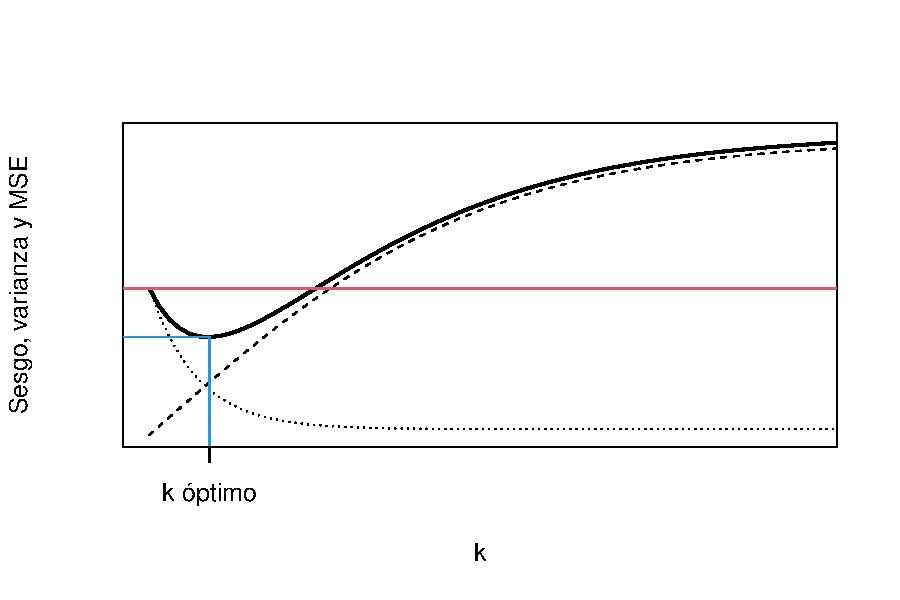
\includegraphics{MLG2_files/figure-latex/ECMrepresentacion-1} 

}

\caption{Representación del sesgo al cuadrado (linea cortada), varianza (linea punteada) y error cuadrático medio (linea solida) del estimador de ridge. La linea roja representa el error cuadrático medio del estimador por MCO.}\label{fig:ECMrepresentacion}
\end{figure}

Algunos métodos de selección de \(k\) son:

\begin{itemize}
\item
  Traza de ridge \(k\): el efecto de \(k\) sobre las estimaciones de \(\widehat{\boldsymbol b}_{R}\) es mas fuerte para valores bajos. De igual forma, si \(k\) es muy grande introducimos mucho sesgo. Por lo que se puede hacer es incrementar \(k\) hasta que parezca que su influencia sobre \(\widehat{\boldsymbol b}_{R}\) se atenúe.
\item
  Validación cruzada (CV): sea \(\widehat{y}_{(i),k}\) la estimación de \(E(y_i)\) por medio del estimador de ridge con el parámetro \(k\) y usando una muestra excluyendo la i-ésima observación. La validación cruzada está definida como:
  \[
  CV(k) = \sum_{i=1}^{n} (y_i - \widehat{y}_{(i),k})^2.
  \]
  Por lo que la selección de \(k\) es:
  \[
  k_{CV} = \arg \min_{k} CV(k).
  \]
\end{itemize}

\hypertarget{datos-de-cemento-1}{%
\subsubsection{Datos de cemento}\label{datos-de-cemento-1}}

Para ajustar el modelo usando el estimador de ridge podemos usar la función \texttt{lmridge} del paquete \texttt{lmridge}. Primero, ajustamos el modelo usando diferentes valores de \(k\):

\begin{Shaded}
\begin{Highlighting}[]
\FunctionTok{library}\NormalTok{(lmridge)}
\NormalTok{K }\OtherTok{=} \FunctionTok{seq}\NormalTok{(}\AttributeTok{from=}\DecValTok{0}\NormalTok{,}\AttributeTok{to=}\FloatTok{0.3}\NormalTok{,}\AttributeTok{length.out =} \DecValTok{100}\NormalTok{)}
\NormalTok{ridge.cement }\OtherTok{=} \FunctionTok{lmridge}\NormalTok{(y}\SpecialCharTok{\textasciitilde{}}\NormalTok{., }\AttributeTok{data=}\NormalTok{cement,}\AttributeTok{K=}\NormalTok{K,}\AttributeTok{scaling=}\StringTok{\textquotesingle{}sc\textquotesingle{}}\NormalTok{)}
\end{Highlighting}
\end{Shaded}

En el objeto \texttt{ridge.cement} tenemos las estimaciones por el estimador de ridge para \(100\) valores de \(k\) entre \(0\) y \(0.3\). Para observar como cambian las estimaciones para los diferentes valores de \(k\) podemos graficar la traza de ridge así (en términos de las covariables en su escala orginal):

\begin{Shaded}
\begin{Highlighting}[]
\NormalTok{EstRidge.cement }\OtherTok{=} \FunctionTok{coef}\NormalTok{(ridge.cement)}
\FunctionTok{plot}\NormalTok{(K,EstRidge.cement[,}\DecValTok{2}\NormalTok{],}\AttributeTok{type=}\StringTok{\textquotesingle{}l\textquotesingle{}}\NormalTok{,}\AttributeTok{ylim=}\FunctionTok{range}\NormalTok{(EstRidge.cement[,}\SpecialCharTok{{-}}\DecValTok{1}\NormalTok{]),}\AttributeTok{lwd=}\DecValTok{2}\NormalTok{,}
     \AttributeTok{ylab=}\StringTok{\textquotesingle{}Estimaciones de los coeficientes\textquotesingle{}}\NormalTok{,}\AttributeTok{xlab=}\StringTok{\textquotesingle{}k\textquotesingle{}}\NormalTok{)}
\FunctionTok{lines}\NormalTok{(K,EstRidge.cement[,}\DecValTok{3}\NormalTok{],}\AttributeTok{col=}\DecValTok{2}\NormalTok{,}\AttributeTok{lwd=}\DecValTok{2}\NormalTok{)}
\FunctionTok{lines}\NormalTok{(K,EstRidge.cement[,}\DecValTok{4}\NormalTok{],}\AttributeTok{col=}\DecValTok{3}\NormalTok{,}\AttributeTok{lwd=}\DecValTok{2}\NormalTok{)}
\FunctionTok{lines}\NormalTok{(K,EstRidge.cement[,}\DecValTok{5}\NormalTok{],}\AttributeTok{col=}\DecValTok{4}\NormalTok{,}\AttributeTok{lwd=}\DecValTok{2}\NormalTok{)}
\FunctionTok{abline}\NormalTok{(}\AttributeTok{h=}\DecValTok{0}\NormalTok{,}\AttributeTok{lty=}\DecValTok{2}\NormalTok{)}
\end{Highlighting}
\end{Shaded}

\begin{figure}

{\centering 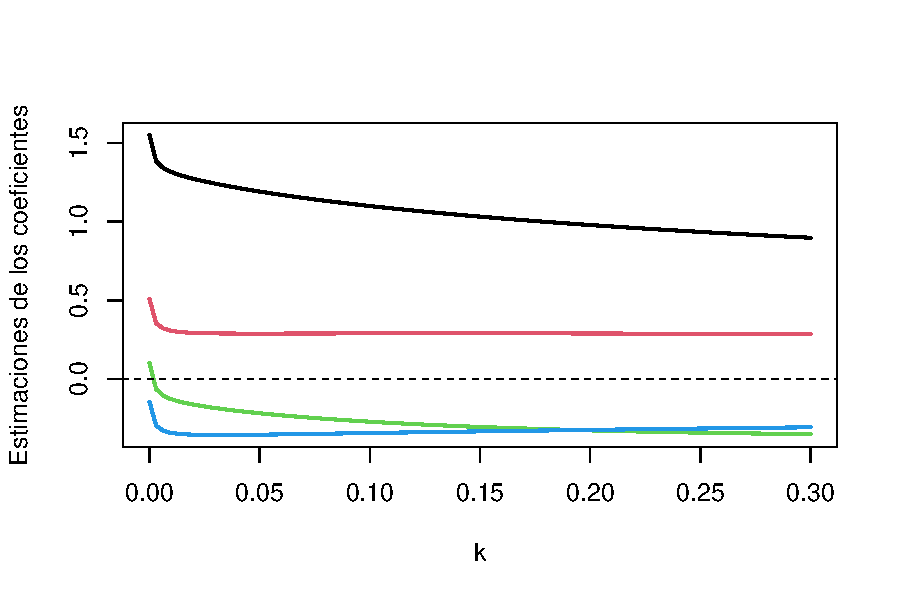
\includegraphics{MLG2_files/figure-latex/CementTrazaRidge-1} 

}

\caption{Datos de cemento. Traza de ridge. Coeficiente asociado a ``X1`` (negro), coeficiente asociado a ``X2`` (rojo), coeficiente asociado a ``X3`` (verde) y coeficiente asociado a ``X4`` (azul)}\label{fig:CementTrazaRidge}
\end{figure}

En la Figura \ref{fig:CementTrazaRidge} podemos observar que, cuando incrementamos \(k\), las estimaciones cambian rápidamente y luego parecen estabilizarse cuando \(k\) es grande. Además hay un cambio de signo para el coeficiente asociado a \texttt{X3}. También puede usarse \texttt{plot(mod.r)} (traza de ridge para las estimaciones de los coeficientes asociados a las covariables escaladas).

La selección del \(k\) óptimo por medio de validación cruzada (CV) se hace de la siguiente manera:

\begin{Shaded}
\begin{Highlighting}[]
\NormalTok{Criterios.cement }\OtherTok{=} \FunctionTok{kest}\NormalTok{(ridge.cement)}
\FunctionTok{plot}\NormalTok{(K,Criterios.cement}\SpecialCharTok{$}\NormalTok{CV,}\AttributeTok{type=}\StringTok{\textquotesingle{}l\textquotesingle{}}\NormalTok{,}\AttributeTok{xlab=}\StringTok{\textquotesingle{}K\textquotesingle{}}\NormalTok{,}\AttributeTok{ylab=}\StringTok{\textquotesingle{}validación cruzada\textquotesingle{}}\NormalTok{)}
\end{Highlighting}
\end{Shaded}

\begin{figure}

{\centering 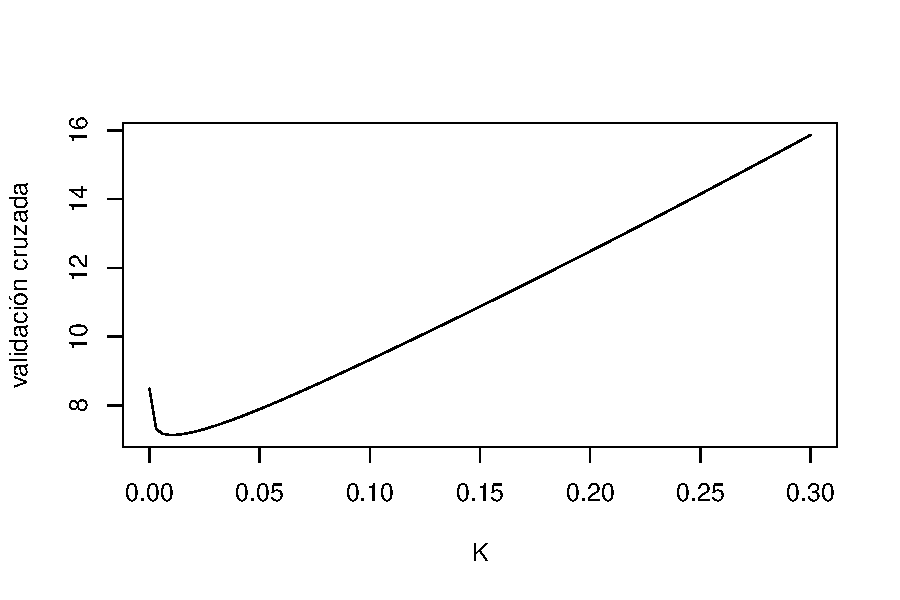
\includegraphics{MLG2_files/figure-latex/cementridge3-1} 

}

\caption{\label{fig:CementCVridge} Datos de cemento. Validación cruzada.}\label{fig:cementridge3}
\end{figure}

\begin{Shaded}
\begin{Highlighting}[]
\NormalTok{K[Criterios.cement}\SpecialCharTok{$}\NormalTok{CV}\SpecialCharTok{==}\FunctionTok{min}\NormalTok{(Criterios.cement}\SpecialCharTok{$}\NormalTok{CV)]}
\end{Highlighting}
\end{Shaded}

\begin{verbatim}
## [1] 0.009090909
\end{verbatim}

Aquí podemos ver que el valorde \(k\) que minimiza la validación cruzada es \(0.009\). El valor óptimo de \(k\) por medio de otros criterios son:

\begin{Shaded}
\begin{Highlighting}[]
\NormalTok{Criterios.cement}
\end{Highlighting}
\end{Shaded}

\begin{verbatim}
## Ridge k from different Authors
## 
##                                k values
## Thisted (1976):                 0.00581
## Dwividi & Srivastava (1978):    0.00291
## LW (lm.ridge)                   0.05183
## LW (1976)                       0.00797
## HKB (1975)                      0.01162
## Kibria (2003) (AM)              0.28218
## Minimum GCV at                  0.02424
## Minimum CV at                   0.00909
## Kibria 2003 (GM):               0.07733
## Kibria 2003 (MED):              0.01718
## Muniz et al. 2009 (KM2):       14.84574
## Muniz et al. 2009 (KM3):        5.32606
## Muniz et al. 2009 (KM4):        3.59606
## Muniz et al. 2009 (KM5):        0.27808
## Muniz et al. 2009 (KM6):        7.80532
## Mansson et al. 2012 (KMN8):    14.98071
## Mansson et al. 2012 (KMN9):     0.49624
## Mansson et al. 2012 (KMN10):    6.63342
## Mansson et al. 2012 (KMN11):    0.15075
## Mansson et al. 2012 (KMN12):    8.06268
## Dorugade et al. 2010:           0.00000
## Dorugade et al. 2014:         101.64433
\end{verbatim}

La estimación con \(K=0.0101\) se puede obtener usando la función \texttt{lmridge} usando \(K=0.0101\) como argumento:

\begin{Shaded}
\begin{Highlighting}[]
\NormalTok{ridge.cement2 }\OtherTok{=} \FunctionTok{lmridge}\NormalTok{(y}\SpecialCharTok{\textasciitilde{}}\NormalTok{., }\AttributeTok{data=}\NormalTok{cement,}\AttributeTok{K=}\FloatTok{0.0101}\NormalTok{,}\AttributeTok{scaling=}\StringTok{\textquotesingle{}sc\textquotesingle{}}\NormalTok{)}
\FunctionTok{summary}\NormalTok{(ridge.cement2)}
\end{Highlighting}
\end{Shaded}

\begin{verbatim}
## 
## Call:
## lmridge.default(formula = y ~ ., data = cement, K = 0.0101, scaling = "sc")
## 
## 
## Coefficients: for Ridge parameter K= 0.0101 
##            Estimate Estimate (Sc) StdErr (Sc) t-value (Sc) Pr(>|t|)    
## Intercept   82.7052     -267.6034    306.3344      -0.8736   0.4052    
## x1           1.3146       26.7886      3.9606       6.7637   0.0001 ***
## x2           0.3059       16.4871      5.2766       3.1246   0.0124 *  
## x3          -0.1295       -2.8734      3.9360      -0.7300   0.4841    
## x4          -0.3432      -19.8985      5.4000      -3.6849   0.0051 ** 
## ---
## Signif. codes:  0 '***' 0.001 '**' 0.01 '*' 0.05 '.' 0.1 ' ' 1
## 
## Ridge Summary
##        R2    adj-R2  DF ridge         F       AIC       BIC 
##   0.97180   0.96240   3.07629 133.92403  23.27712  58.35941 
## Ridge minimum MSE= 392.3519 at K= 0.0101 
## P-value for F-test ( 3.07629 , 9.74488 ) = 3.013147e-08 
## -------------------------------------------------------------------
\end{verbatim}

Vemos algunas diferencias con las estimaciones por MCO. Hay un cambio de signo en la estimación del coeficiente asociado a \texttt{x3}. Si embargo, no hay mucha diferencia en las estimaciones de los otros coeficientes. También podemos observar que las covariables \texttt{x1}, \texttt{x2} y \texttt{x3} ahora tienen un aporte significativo. Como era de esperarse, hay una disminución del \(R^{2}\), sin embargo es muy leve.

\hypertarget{estimador-por-componentes-principales}{%
\subsection{Estimador por componentes principales}\label{estimador-por-componentes-principales}}

Considere el modelo en su forma canónica:
\[
\boldsymbol y^{*} = \boldsymbol Z\boldsymbol T\boldsymbol \alpha+ \boldsymbol \varepsilon,
\]
donde \(\boldsymbol \alpha= \boldsymbol T'\boldsymbol b\), \((\boldsymbol Z\boldsymbol T)'\boldsymbol Z\boldsymbol T=\boldsymbol \Lambda\), \(\boldsymbol \Lambda\) es una matriz diagonal de valores propios \((\lambda_1,\ldots,\lambda_p)\) de \(\boldsymbol Z'\boldsymbol Z\), y \(\boldsymbol T= (\boldsymbol t_{1},\ldots,\boldsymbol t_{p-1})\) es la matriz ortogonal de vectores propios asociados \(\boldsymbol \Lambda\).

Las columnas de \(\boldsymbol P= \boldsymbol Z\boldsymbol T= (\boldsymbol p_{1},\ldots,\boldsymbol p_{p-1})\) son un conjunto de regresores ortogonales(llamados componentes principales):
\[
\boldsymbol p_{k} = \sum_{j=1}^{p-1} t_{kj}\boldsymbol z_{j}.
\]
El estimador de \(\boldsymbol \alpha\) por MCO es:
\[
\widehat{\boldsymbol \alpha}= (\boldsymbol P'\boldsymbol P)^{-1}\boldsymbol P'\boldsymbol y^{*} = \boldsymbol \Lambda^{-1}\boldsymbol P'\boldsymbol y^{*},
\]
y la varianza de \(\widehat{\boldsymbol \alpha}\) es:
\[
V(\widehat{\boldsymbol \alpha}) = \sigma^{2}(\boldsymbol P'\boldsymbol P)^{-1} = \sigma^{2}\boldsymbol \Lambda^{-1}.
\]
De aquí podemos ver que valores propios de \(\boldsymbol Z'\boldsymbol Z\) están asociados con la varianza de los coeficientes de regresión. Si \(\lambda_j=1\) (para \(j=1,\ldots,p\)), las covariables originales son ortogonales. Mientras que valores propios cercanos a cero indican problemas de multicolinealidad dado que inflan la varianza de \(\widehat{\boldsymbol \alpha}\).

Además, Note que para \(\widehat{\boldsymbol b}= \boldsymbol T\widehat{\boldsymbol \alpha}\), tenemos:
\[
V(\widehat{\boldsymbol b}) = V(\boldsymbol T\widehat{\boldsymbol \alpha}) =\sigma^{2}\boldsymbol T\boldsymbol \Lambda^{-1}\boldsymbol T' = \sigma^{2} \sum_{j=1}^{p-1}\lambda_{j}^{-1}\boldsymbol t_{j}\boldsymbol t_{j}',
\]
lo que implica que \(V(\widehat{b}_{k}) = \sigma^{2} \sum_{j=1}^{p-1}t_{kj}^{2}/\lambda_{j}\); la varianza de \(\widehat{b}_j\) es una combinación lineal de los valores propios.

Para combatir el problema de multicolinealidad, la idea de la regresión por componentes principales es usar un subconjunto de \(\boldsymbol P\) como regresores (en vez de todos los compontes). Para esto, eliminamos los componentes principales \((\boldsymbol p_{r+1},\ldots,\boldsymbol p_{p-1})\) asociados a los valores propios cercanos a cero \((\lambda_{r+1},\ldots,\lambda_{p-1})\). Aquí estamos asumiendo que los valores propios están ordenados de mayor a menor, \(\lambda_1 \leq \lambda_2 \leq \ldots \leq \lambda_p\) (como lo hace \texttt{R}). Esto es,
\[
\widehat{\boldsymbol \alpha}_{PC} = \boldsymbol L\widehat{\boldsymbol \alpha}= \begin{pmatrix} \boldsymbol I_{r} & \boldsymbol 0\\ \boldsymbol 0& \boldsymbol 0\end{pmatrix} \widehat{\boldsymbol \alpha}.
\]
Por lo tanto \(\widehat{\boldsymbol \alpha}_{PC} = (\overbrace{\widehat{\alpha}_{1},\widehat{\alpha}_{2},\ldots, \widehat{\alpha}_{r}}^{r},\overbrace{0, \ldots,0}^{p-1-r})'\).

En términos de \(\boldsymbol b\),
\[
\widehat{\boldsymbol b}_{PC} = \boldsymbol T\widehat{\boldsymbol \alpha}_{PC} = \boldsymbol T\boldsymbol L\boldsymbol \Lambda^{-1}\boldsymbol T'\boldsymbol Z'\boldsymbol y^{*}.
\]
Además,
\[
V(\widehat{\boldsymbol b}_{PC}) = \sigma^{2} \boldsymbol T\boldsymbol L\boldsymbol \Lambda^{-1}\boldsymbol L'\boldsymbol T' = \sigma^{2}\sum_{j=1}^{r} \lambda_{j}^{-1}\boldsymbol t_{j}\boldsymbol t_{j}'.
\]
lo que implica que \(V(\widehat{b}_{PC,j}) = \sigma^{2} \sum_{k=1}^{r}t_{jk}^{2}/\lambda_{k}\).

El sesgo de \(\widehat{\boldsymbol b}_{PC}\) está definido como:
\[
E(\boldsymbol T\widehat{\boldsymbol \alpha}_{PC}) - \boldsymbol T\boldsymbol \alpha= -\sum_{k=r+1}^{p-1}\alpha_k\boldsymbol t_{k}.
\]
Mientras que la varianza de \(\widehat{\boldsymbol b}_{PC}\) es:
\begin{equation}
V(\boldsymbol T\widehat{\boldsymbol \alpha}_{PC}) = \boldsymbol T\left[ \sigma^{2}\boldsymbol L\boldsymbol \Lambda^{-1} \boldsymbol L\right] \boldsymbol T^{-1} = \sigma^{2} \sum_{k=1}^{r}\lambda_k^{-1}\boldsymbol t_{k}\boldsymbol t_{k}' \leq \sigma^{2} \sum_{k=1}^{p-1}\lambda_k^{-1}\boldsymbol t_{k}\boldsymbol t_{k}' = \sigma^{2}(\boldsymbol Z'\boldsymbol Z)^{-1}.
\label{eq:varBPC}
\end{equation}
Por lo tanto, al eliminar componentes principales se aumenta el sesgo, pero se disminuye la varianza de \(\widehat{\boldsymbol b}_{PC}\).

Note en \eqref{eq:varBPC} que la diferencia en varianzas con respecto al estimador de MCO de \(\boldsymbol b\):
\[
\sigma^{2}\sum_{k=r+1}^{p-1}\lambda_k^{-1} \boldsymbol t_{k}\boldsymbol t_{k}',
\]
será mayor si las componentes principales excluidas están asociadas a valores propios pequeños.

\hypertarget{datos-de-cemento-2}{%
\subsubsection{Datos de cemento}\label{datos-de-cemento-2}}

Antes de ajustar el modelo vamos a escalar las variables

\begin{Shaded}
\begin{Highlighting}[]
\NormalTok{escalar }\OtherTok{\textless{}{-}} \ControlFlowTok{function}\NormalTok{(x) \{(x}\SpecialCharTok{{-}}\FunctionTok{mean}\NormalTok{(x)) }\SpecialCharTok{/} \FunctionTok{sqrt}\NormalTok{(}\FunctionTok{sum}\NormalTok{((x}\SpecialCharTok{{-}}\FunctionTok{mean}\NormalTok{(x))}\SpecialCharTok{\^{}}\DecValTok{2}\NormalTok{))\}}
\NormalTok{X }\OtherTok{=} \FunctionTok{as.matrix}\NormalTok{(cement[,}\DecValTok{1}\SpecialCharTok{:}\DecValTok{4}\NormalTok{])}
\NormalTok{y.e }\OtherTok{=} \FunctionTok{escalar}\NormalTok{(cement}\SpecialCharTok{$}\NormalTok{y)}
\NormalTok{Z }\OtherTok{=} \FunctionTok{apply}\NormalTok{(cement[,}\DecValTok{1}\SpecialCharTok{:}\DecValTok{4}\NormalTok{],}\DecValTok{2}\NormalTok{,escalar)}
\end{Highlighting}
\end{Shaded}

A partir de las variables escaladas podemos calcular los vectores y valores propios:

\begin{Shaded}
\begin{Highlighting}[]
\NormalTok{T.mat }\OtherTok{=} \FunctionTok{eigen}\NormalTok{(}\FunctionTok{t}\NormalTok{(Z)}\SpecialCharTok{\%*\%}\NormalTok{Z)}\SpecialCharTok{$}\NormalTok{vectors}
\NormalTok{lambda }\OtherTok{=} \FunctionTok{eigen}\NormalTok{(}\FunctionTok{t}\NormalTok{(Z)}\SpecialCharTok{\%*\%}\NormalTok{Z)}\SpecialCharTok{$}\NormalTok{values}
\NormalTok{lambda}
\end{Highlighting}
\end{Shaded}

\begin{verbatim}
## [1] 2.235704035 1.576066070 0.186606149 0.001623746
\end{verbatim}

Aquí podemos observar que un valor propio es cercano a cero, por lo que lo podemos eliminarlo para remediar el problema de multicolinealidad:

\begin{Shaded}
\begin{Highlighting}[]
\NormalTok{P }\OtherTok{=}\NormalTok{ Z}\SpecialCharTok{\%*\%}\NormalTok{T.mat}
\NormalTok{PCR.cement }\OtherTok{=} \FunctionTok{lm}\NormalTok{(y.e}\SpecialCharTok{\textasciitilde{}}\NormalTok{P[,}\SpecialCharTok{{-}}\DecValTok{4}\NormalTok{]}\SpecialCharTok{{-}}\DecValTok{1}\NormalTok{)}
\FunctionTok{summary}\NormalTok{(PCR.cement)}
\end{Highlighting}
\end{Shaded}

\begin{verbatim}
## 
## Call:
## lm(formula = y.e ~ P[, -4] - 1)
## 
## Residuals:
##       Min        1Q    Median        3Q       Max 
## -0.058393 -0.036851  0.006961  0.022836  0.073963 
## 
## Coefficients:
##           Estimate Std. Error t value Pr(>|t|)    
## P[, -4]1 -0.656958   0.028271 -23.238 4.93e-10 ***
## P[, -4]2 -0.008309   0.033671  -0.247   0.8101    
## P[, -4]3  0.302770   0.097856   3.094   0.0114 *  
## ---
## Signif. codes:  0 '***' 0.001 '**' 0.01 '*' 0.05 '.' 0.1 ' ' 1
## 
## Residual standard error: 0.04227 on 10 degrees of freedom
## Multiple R-squared:  0.9821, Adjusted R-squared:  0.9768 
## F-statistic: 183.2 on 3 and 10 DF,  p-value: 4.895e-09
\end{verbatim}

Las estimaciones de los coeficientes \((\boldsymbol b)\) para las variables escaladas:

\begin{Shaded}
\begin{Highlighting}[]
\NormalTok{beta.CP }\OtherTok{=}\NormalTok{T.mat}\SpecialCharTok{\%*\%}\FunctionTok{c}\NormalTok{(PCR.cement}\SpecialCharTok{$}\NormalTok{coefficients,}\DecValTok{0}\NormalTok{)}
\NormalTok{beta.CP}
\end{Highlighting}
\end{Shaded}

\begin{verbatim}
##             [,1]
## [1,]  0.51297502
## [2,]  0.27868114
## [3,] -0.06078483
## [4,] -0.42288461
\end{verbatim}

La matriz de varianza de \(\boldsymbol b_{PC}\) es:

\begin{Shaded}
\begin{Highlighting}[]
\NormalTok{sigma2.pc }\OtherTok{=} \FunctionTok{sum}\NormalTok{(PCR.cement}\SpecialCharTok{$}\NormalTok{residuals}\SpecialCharTok{\^{}}\DecValTok{2}\NormalTok{)}\SpecialCharTok{/}\NormalTok{(}\DecValTok{13{-}4}\NormalTok{)}
\NormalTok{Var.b }\OtherTok{=}\NormalTok{ sigma2.pc}\SpecialCharTok{*}\NormalTok{T.mat}\SpecialCharTok{\%*\%}\FunctionTok{diag}\NormalTok{(}\FunctionTok{c}\NormalTok{(}\DecValTok{1}\SpecialCharTok{/}\NormalTok{lambda[}\DecValTok{1}\SpecialCharTok{:}\DecValTok{3}\NormalTok{],}\DecValTok{0}\NormalTok{))}\SpecialCharTok{\%*\%}\FunctionTok{t}\NormalTok{(T.mat)}
\NormalTok{Var.b}
\end{Highlighting}
\end{Shaded}

\begin{verbatim}
##              [,1]          [,2]         [,3]          [,4]
## [1,]  0.005382414 -0.0022868445  0.004028698 -0.0013467849
## [2,] -0.002286844  0.0015500408 -0.002015159  0.0001440783
## [3,]  0.004028698 -0.0020151593  0.004925579 -0.0014780352
## [4,] -0.001346785  0.0001440783 -0.001478035  0.0009294415
\end{verbatim}

\hypertarget{selecciuxf3n-de-variables}{%
\section{Selección de variables}\label{selecciuxf3n-de-variables}}

\hypertarget{ejemplos-3}{%
\subsection{Ejemplos}\label{ejemplos-3}}

\hypertarget{unidad-quiruxfargica}{%
\subsubsection{Unidad quirúrgica}\label{unidad-quiruxfargica}}

Una unidad quirúrgica de un hospital está interesada en predecir la supervivencia de los pacientes sometidos a un tipo particular de operación hepática. Se dispuso de una selección aleatoria de \(108\) pacientes para el análisis. De cada registro del paciente, se extrajo la siguiente información de la evaluación preoperatoria:

\begin{itemize}
\item
  \texttt{bcs}: coagulación sanguínea.
\item
  \texttt{pindex}: índice de pronóstico.
\item
  \texttt{enzyme}: función enzimática.
\item
  \texttt{liver\_test}: función hepática.
\item
  \texttt{age}: edad.
\item
  \texttt{gender}: genero (0 = masculino, 1 = femenino).
\item
  \texttt{alc\_mod}: historial de consumo de alcohol (0 = Ninguno, 1 = Moderado).
\item
  \texttt{alc\_heavy}: \& historial de consumo de alcohol (0 = Ninguno, 1 = Fuerte).
\item
  \texttt{y}: tiempo de supervivencia.
\end{itemize}

El objetivo del estudio es determinar los factores que influyen sobre el tiempo de supervivencia (que se determinó posteriormente) en función de las demás variables.

El modelo propuesto es el siguiente:
\begin{equation}
\begin{split}
\log y_{i} =& \beta_{0}+\mbox{bcs}_{i}\beta_{1} + \mbox{pindex}_{i}\beta_{2}+ \mbox{enzyme}_{i}\beta_{3} +  \mbox{liver}_{i}\beta_{4} + \mbox{age}_{i}\beta_{5} +  \mbox{gender}_{i}\beta_{6}+ \\ & \mbox{alc_mod}_{i}\beta_{7} + \mbox{alc_heavy}_{i}\beta_{8} + \varepsilon_{i}
\end{split}
\nonumber
\end{equation}

El ajuste del modelo es:

\begin{Shaded}
\begin{Highlighting}[]
\FunctionTok{library}\NormalTok{(olsrr)}
\FunctionTok{data}\NormalTok{(surgical)}
\NormalTok{mod.surgical.completo }\OtherTok{=} \FunctionTok{lm}\NormalTok{(}\FunctionTok{log}\NormalTok{(y)}\SpecialCharTok{\textasciitilde{}}\NormalTok{.,}\AttributeTok{data=}\NormalTok{surgical)}
\FunctionTok{summary}\NormalTok{(mod.surgical.completo)}
\end{Highlighting}
\end{Shaded}

\begin{verbatim}
## 
## Call:
## lm(formula = log(y) ~ ., data = surgical)
## 
## Residuals:
##      Min       1Q   Median       3Q      Max 
## -0.35555 -0.13849 -0.05179  0.14912  0.46349 
## 
## Coefficients:
##              Estimate Std. Error t value Pr(>|t|)    
## (Intercept)  4.050949   0.251741  16.092  < 2e-16 ***
## bcs          0.068551   0.025420   2.697  0.00982 ** 
## pindex       0.013459   0.001947   6.913 1.37e-08 ***
## enzyme_test  0.014948   0.001809   8.261 1.44e-10 ***
## liver_test   0.007931   0.046706   0.170  0.86592    
## age         -0.003567   0.002751  -1.296  0.20145    
## gender       0.084151   0.060746   1.385  0.17279    
## alc_mod      0.057313   0.067480   0.849  0.40019    
## alc_heavy    0.388190   0.088374   4.393 6.73e-05 ***
## ---
## Signif. codes:  0 '***' 0.001 '**' 0.01 '*' 0.05 '.' 0.1 ' ' 1
## 
## Residual standard error: 0.2093 on 45 degrees of freedom
## Multiple R-squared:  0.8461, Adjusted R-squared:  0.8187 
## F-statistic: 30.93 on 8 and 45 DF,  p-value: 7.823e-16
\end{verbatim}

\hypertarget{grasa-corporal-1}{%
\subsubsection{Grasa corporal}\label{grasa-corporal-1}}

La medición de la grasa corporal es un proceso complejo. Dado que los músculos y los huesos son más densos, el calculo de \% de grasa corporal se basa, entre otros aspectos, en la medición de la densidad corporal la cuál requiere sumergir a las personas en el agua.

Por esta razón se quiere buscar un método más sencillo para determinar el \% de grasa corporal. Para esto, se registraron la edad, el peso, la altura y \(10\) medidas de la circunferencia corporal de \(252\) hombres. De igual forma, a cada uno de estos hombres se les midió el \% de grasa corporal de forma precisa (usando la ecuación de Brozek, medición a partir de la densidad).

Cómo variable respuesta se utiliza la medición por el método de Brozek, y las posibles covariables son:

\begin{itemize}
\item
  \texttt{age}: edad (en años).
\item
  \texttt{weight}: peso (en libras).
\item
  \texttt{height}: altura (en pulgadas).
\item
  \texttt{neck}: circunferencia del cuello (en centímetros).
\item
  \texttt{chest}: circunferencia del pecho (en centímetros).
\item
  \texttt{abdom}: circunferencia del abdomen (en centímetros).
\item
  \texttt{hip}: circunferencia de la cadera (en centímetros).
\item
  \texttt{thigh}:circunferencia del muslo (en centímetros).
\item
  \texttt{knee}:circunferencia de la rodilla (en centímetros).
\item
  \texttt{ankle}:circunferencia del tobillo (en centímetros).
\item
  \texttt{biceps}: circunferencia del bíceps extendido (en centímetros).
\item
  \texttt{forearm}: circunferencia del antebrazo (en centímetros).
\item
  ``wrist```: circunferencia de la muñeca (en centímetros).
\end{itemize}

El modelo propuesto es el siguiente:
\[
\mbox{brozek}_i = \beta_{0} + \mbox{age}_i\beta_1+ \mbox{weight}_i\beta_2 + \ldots + \mbox{wrist}_i\beta_{13}  + \varepsilon_i.
\]
El ajuste del modelo es:

\begin{Shaded}
\begin{Highlighting}[]
\FunctionTok{library}\NormalTok{(faraway)}
\FunctionTok{data}\NormalTok{(fat)}
\NormalTok{mod.fat }\OtherTok{\textless{}{-}} \FunctionTok{lm}\NormalTok{(brozek }\SpecialCharTok{\textasciitilde{}}\NormalTok{ age }\SpecialCharTok{+}\NormalTok{ weight }\SpecialCharTok{+}\NormalTok{ height }\SpecialCharTok{+}\NormalTok{ neck }\SpecialCharTok{+}\NormalTok{ chest }\SpecialCharTok{+}\NormalTok{ abdom }\SpecialCharTok{+}
\NormalTok{             hip }\SpecialCharTok{+}\NormalTok{ thigh }\SpecialCharTok{+}\NormalTok{ knee }\SpecialCharTok{+}\NormalTok{ ankle }\SpecialCharTok{+}\NormalTok{ biceps }\SpecialCharTok{+}\NormalTok{ forearm }\SpecialCharTok{+}\NormalTok{ wrist, }\AttributeTok{data=}\NormalTok{fat)}
\FunctionTok{summary}\NormalTok{(mod.fat)}
\end{Highlighting}
\end{Shaded}

\begin{verbatim}
## 
## Call:
## lm(formula = brozek ~ age + weight + height + neck + chest + 
##     abdom + hip + thigh + knee + ankle + biceps + forearm + wrist, 
##     data = fat)
## 
## Residuals:
##     Min      1Q  Median      3Q     Max 
## -10.264  -2.572  -0.097   2.898   9.327 
## 
## Coefficients:
##              Estimate Std. Error t value Pr(>|t|)    
## (Intercept) -15.29255   16.06992  -0.952  0.34225    
## age           0.05679    0.02996   1.895  0.05929 .  
## weight       -0.08031    0.04958  -1.620  0.10660    
## height       -0.06460    0.08893  -0.726  0.46830    
## neck         -0.43754    0.21533  -2.032  0.04327 *  
## chest        -0.02360    0.09184  -0.257  0.79740    
## abdom         0.88543    0.08008  11.057  < 2e-16 ***
## hip          -0.19842    0.13516  -1.468  0.14341    
## thigh         0.23190    0.13372   1.734  0.08418 .  
## knee         -0.01168    0.22414  -0.052  0.95850    
## ankle         0.16354    0.20514   0.797  0.42614    
## biceps        0.15280    0.15851   0.964  0.33605    
## forearm       0.43049    0.18445   2.334  0.02044 *  
## wrist        -1.47654    0.49552  -2.980  0.00318 ** 
## ---
## Signif. codes:  0 '***' 0.001 '**' 0.01 '*' 0.05 '.' 0.1 ' ' 1
## 
## Residual standard error: 3.988 on 238 degrees of freedom
## Multiple R-squared:  0.749,  Adjusted R-squared:  0.7353 
## F-statistic: 54.63 on 13 and 238 DF,  p-value: < 2.2e-16
\end{verbatim}

\hypertarget{problema-de-selecciuxf3n-de-variables}{%
\subsection{Problema de selección de variables}\label{problema-de-selecciuxf3n-de-variables}}

En problemas de regresión se tiene un conjunto grande de potenciales covariables. Si ajustamos un modelo considerandolas todas podemos estar incluyendo covariables que son irrelevante. Por el otro lado, si no las incluimos todas es posible que estemos omitiendo covariables importantes. En ambos casos hay consecuencias negativas.

Para illustrar esto, considere el siguiente modelo:
\begin{equation}
\begin{split}
y_{i} &= \beta_{0} + \sum_{j=1}^{p-1}\beta_{j}x_{ij} + \varepsilon_{i} \\
&= \beta_{0} + \sum_{j=1}^{r}\beta_{j}x_{ij} + \sum_{j=r+1}^{p-1}\beta_{j}x_{ij} + \varepsilon_{i} \\
&= \boldsymbol x_{1i}'\boldsymbol \beta_1 + \boldsymbol x_{2i}'\boldsymbol \beta_2 + \varepsilon_i,
\end{split}
\label{eq:modelogral}
\end{equation}
donde \(\boldsymbol x_{1i} = (1,x_{1i},x_{2i},\ldots,x_{ri})\), \(\boldsymbol x_{2i} = (x_{r+1,i},x_{r+2,i},\ldots,x_{p-1,i})\), \(\boldsymbol \beta_1 = (\beta_0,\beta_1,\beta_2,\ldots,\beta_r)'\), \(\boldsymbol \beta_2 = (\beta_{r+1},\beta_{r+2},\ldots,\beta_{p-1})'\), y \(\varepsilon_i \sim N(0,\sigma^{2})\). Es decir, se hace una partición de las covariables y los coeficientes de regressión en dos componentes.

En forma matricial, el modelo es:
\[
\boldsymbol y= \boldsymbol X_{1}\boldsymbol \beta_{1} + \boldsymbol X_{2}\boldsymbol \beta_{2}+ \boldsymbol \varepsilon,
\]
donde \(\boldsymbol X_{1}\) es una matriz \(n \times r\) con la \(i\)-ésima fila igual a \(\boldsymbol x_{1i}\) y \(\boldsymbol X_{2}\) es una matriz \(n \times (p-r-1)\) con la \(i\)-ésima fila igual a \(\boldsymbol x_{2i}\).

\hypertarget{quuxe9-pasa-si-ignoramos-covariables-importantes}{%
\subsubsection{¿Qué pasa si ignoramos covariables importantes?}\label{quuxe9-pasa-si-ignoramos-covariables-importantes}}

Ahora, considere que el modelo de regresión real es \eqref{eq:modelogral}, pero decidimos estimar:
\[
y_{i} = \boldsymbol x_{1i}'\boldsymbol \beta_1 + \varepsilon_i.
\]
Por lo tanto, estamos omitiendo las covariables \(\boldsymbol x_{2i}\) del modelo (puesto que \(\boldsymbol \beta_2 \neq 0\)).

El estimador por MCO de \(\boldsymbol \beta_1\) es:
\[
\widehat{\boldsymbol \beta}_{1} = (\boldsymbol X_{1}'\boldsymbol X_{1})^{-1}\boldsymbol X_{1}'\boldsymbol y.
\]
De aquí tenemos que \(E(\widehat{\boldsymbol \beta}_{1}) = \boldsymbol \beta_{1} + (\boldsymbol X_{1}'\boldsymbol X_{1})^{-1}\boldsymbol X_{1}'\boldsymbol X_{2}\boldsymbol \beta_{2}\). Es decir que \(\widehat{\boldsymbol \beta}_{1}\) es un estimador sesgado, a menos que \(\boldsymbol X_{1}'\boldsymbol X_{2} = \boldsymbol 0\) (las columnas de \(X_{1}\) son ortogonales a las columnas de \(X_{2}\)).

De igual forma, las predicciones también serán sesgadas. La predicción en el punto \(\boldsymbol x_{01}\) es:
\[
\widehat{y}_{0} = \boldsymbol x_{01}'\widehat{\boldsymbol \beta}_{1}.
\]
Su valor esperado es:
\[
E(\widehat{y}_{0}) = \boldsymbol x_{01}'\boldsymbol \beta_{1} + \boldsymbol x_{01}'(\boldsymbol X_{1}'\boldsymbol X_{1})^{-1}\boldsymbol X_{1}'\boldsymbol X_{2}\boldsymbol \beta_{2} \neq \boldsymbol x_{01}'\beta_{1} + \boldsymbol x_{02}'\beta_{2}.
\]
Por lo tanto, si omitimos variables relevantes obtenemos sesgo en las estimaciones.

\hypertarget{que-pasa-si-incluimos-covariables-irrelevantes}{%
\subsubsection{¿Que pasa si incluimos covariables irrelevantes?}\label{que-pasa-si-incluimos-covariables-irrelevantes}}

Ahora, consideremos el caso en que \(\boldsymbol \beta_2=0\), es decir, las covariables \(\boldsymbol x_{2}\) no tienen un aporte significativo en el modelo. Pero decidimos estimar el modelo completo.

En este caso, el estimador de \(\boldsymbol \beta\) es:
\[
\widehat{\boldsymbol \beta}= (\boldsymbol X'\boldsymbol X)^{-1}\boldsymbol X'\boldsymbol y= \begin{pmatrix}
\boldsymbol X_{1}'\boldsymbol X_{1} & \boldsymbol X_{1}\boldsymbol X_{2} \\ \boldsymbol X_{2}'\boldsymbol X_{1} & \boldsymbol X_{2}'\boldsymbol X_{2}
\end{pmatrix}^{-1} \begin{pmatrix}
\boldsymbol X_{1}' \\ \boldsymbol X_{2}'
\end{pmatrix}\boldsymbol y.
\]
El Valor esperado de \(\widehat{\boldsymbol \beta}\) es:
\begin{equation}
\begin{split}
E(\widehat{\boldsymbol \beta}) =& (\boldsymbol X'\boldsymbol X)^{-1}\boldsymbol X'E(\boldsymbol y) = (\boldsymbol X'\boldsymbol X)^{-1}\boldsymbol X'\boldsymbol X_{1}\boldsymbol \beta_1 \\
 = & (\boldsymbol X'\boldsymbol X)^{-1}\boldsymbol X'(\boldsymbol X_{1} \ \boldsymbol X_{2}) \begin{pmatrix}
 \boldsymbol \beta_1 \\ \boldsymbol 0
 \end{pmatrix} = \begin{pmatrix}
 \boldsymbol \beta_1 \\ \boldsymbol 0
 \end{pmatrix}.
\end{split}
\nonumber
\end{equation}
Es decir que \(\widehat{\boldsymbol \beta}\) es un estimador insesgado.

La varianza de \(\widehat{\boldsymbol \beta}\) es:
\begin{equation}
\begin{split}
V(\widehat{\boldsymbol \beta}) =& \sigma^{2}(\boldsymbol X'\boldsymbol X)^{-1} = \sigma^{2}\begin{pmatrix}
\boldsymbol X_{1}'\boldsymbol X_{1} & \boldsymbol X_{1}\boldsymbol X_{2} \\ \boldsymbol X_{2}'\boldsymbol X_{1} & \boldsymbol X_{2}'\boldsymbol X_{2}
\end{pmatrix}^{-1} \\
=& \sigma^{2} \begin{pmatrix}
(\boldsymbol X_{1}'\boldsymbol X_{1})^{-1} + \boldsymbol L\boldsymbol M\boldsymbol L& - \boldsymbol L\boldsymbol M\\
-\boldsymbol M\boldsymbol L' & \boldsymbol M
\end{pmatrix},
\end{split}
\nonumber
\end{equation}
donde \(\boldsymbol L= (\boldsymbol X_{1}'\boldsymbol X_{1})^{-1}\boldsymbol X_{1}'\boldsymbol X_{2}\) y \(\boldsymbol M= \boldsymbol X_{2}'(\boldsymbol I- \boldsymbol H_{1})\boldsymbol X_{2}\). Particularmente, para \(\widehat{\boldsymbol \beta}_1\) tenemos que:
\[
V(\widehat{\boldsymbol \beta}_{1}) = \sigma^{2} \left[ (\boldsymbol X_{1}'\boldsymbol X_{1})^{-1} + \boldsymbol L\boldsymbol M\boldsymbol L\right].
\]
Dado que \(\boldsymbol M\) (y por lo tanto \(\boldsymbol L\boldsymbol M\boldsymbol L\)) es positiva-definida, la varianza de \(\widehat{\boldsymbol \beta}_{1}\) se infla al incluir las covariables irrelevantes al modelo. La única excepción es cuando \(\boldsymbol X_{1}\) y \(\boldsymbol X_{2}\) son ortogonales (\(\boldsymbol X_{1}'\boldsymbol X_{2} = \boldsymbol 0\)).

De igual forma, las predicciones en el punto \(\boldsymbol x_{0}' = (\boldsymbol x_{01}' \ \boldsymbol x_{02}')\) son insesgadas:
\[
E(\widehat{y}_{0}) = E(\boldsymbol x_{0}'\widehat{\boldsymbol \beta}) = (\boldsymbol x_{01}' \ \boldsymbol x_{02}')\begin{pmatrix}
\boldsymbol \beta_{1} \\ \boldsymbol 0
\end{pmatrix} = \boldsymbol x_{01}'\boldsymbol \beta_{1}.
\]
Pero su varianza también se infla debido a incluir las covariables irrelevantes:
\[
V(\widehat{y}_{0}) = \sigma^{2} \boldsymbol x_{0}'(\boldsymbol X'\boldsymbol X)^{-1}\boldsymbol x_{0}.
\]

En conclusión:

\begin{itemize}
\item
  Cuando omitimos covariables relevantes, obtenemos sesgos en las estimaciones.
\item
  Cuando incluimos covariables irrelevantes, se inflan las varianzas de las estimaciones. Adicionalmente, incluir más covariables puede llevar a problemas de multicolinealidad.
\end{itemize}

\hypertarget{muxe9todos-para-la-selecciuxf3n-de-variables}{%
\subsection{Métodos para la selección de variables}\label{muxe9todos-para-la-selecciuxf3n-de-variables}}

Si tenemos \((p-1)\) covariables, entonces tenemos \((p-1)^2\) potenciales modelos. Por lo que podemos ajustar todos los posibles modelos y hacer una comparación entre ellos usando algunos criterios de decisión.

Existen varios criterios para determinar que modelo es ``mejor'\,' que otro y este debe escogerse teniendo en cuenta cuál es el objetivo que se tiene al ajustar el modelo (descripción de la relación, predicción, control, etc.). Algunos de estos críterios son:

\begin{itemize}
\tightlist
\item
  Coeficiente de determinación (\(R^{2}\) y \(R^{2}_{adj}\)).
\item
  Estadístico \(C_{p}\) de Mallows.
\item
  Estadístico PRESS y el \(R^{2}\) de predicción.
\item
  Criterios de información (AIC y BIC).
\end{itemize}

\hypertarget{coeficiente-de-determinaciuxf3n}{%
\subsubsection{Coeficiente de determinación}\label{coeficiente-de-determinaciuxf3n}}

Esté indicador está definido como:
\[
R^{2} = \frac{SS_{\mbox{reg}}}{SS_{\mbox{T}}} = 1 - \frac{SS_{\mbox{res}}}{SS_{\mbox{T}}}.
\]
El \(R^{2}\) cuantifica la cantidad de variabilidad de la variable respuesta que es explicada por el modelo. Se tiene que \(0 \leq R^{2} \leq 1\). Valores más cercanos a \(1\) implican que el modelo explica gran parte de la variabilidad de \(y\).

Hay que tener en cuenta que el \(R^{2}\) siempre crece a medida que se adicionan más covariables al modelo. Por lo tanto, se puede puede agregar regresores hasta el punto en que una covariable adicional no propociona un aumento considerable en el \(R^{2}\).

\hypertarget{coeficiente-de-determinaciuxf3n-ajustado}{%
\subsubsection{Coeficiente de determinación ajustado}\label{coeficiente-de-determinaciuxf3n-ajustado}}

Para evitar el incoviente del \(R^{2}\), se puede utlizar el el coeficiente de determinación ajustado definido como:
\[
R^{2}_{adj} = 1 - \frac{n-1}{n-p}\frac{SS_{\mbox{res}}}{SS_{\mbox{T}}} = 1- \frac{MS_{\mbox{res}}}{SS_{\mbox{T}}/(n-1)} = 1- \frac{n-1}{n-p}(1-R^{2}).
\]
El \(R^{2}_{adj}\) no necesariamente aumenta al adicionar nuevos términos al modelo. Este solo aumenta si hay una disminución del \(MS_{\mbox{res}}\).

\hypertarget{c_p-de-mallows}{%
\subsubsection{\texorpdfstring{C\(_p\) de Mallows}{C\_p de Mallows}}\label{c_p-de-mallows}}

Mallows propone un criterio basado en el error cuadrático medio (ECM) de \(\widehat{y}_i\), esto es:
\[
E[\widehat{y}_{i}- E(y_{i})]^2 = [E(y_{i}) - E(\widehat{y}_{i})]^2 + V(\widehat{y}_{i}),
\]
donde \(E(y_{i})\) es el valor esperado de la respuesta (`modelo real'), y \(E(\widehat{y}_{i})\) es el valor esperado de la respuesta basado en el modelo propuesto (basado en \(p\) covariables).

El ECM total estandarizado está definido como:
\begin{equation}
\begin{split}
\Gamma_{p} =& \frac{1}{\sigma^{2}}\left\{\sum_{i=1}^{n}[E(y_{i}) - E(\widehat{y}_{i})]^2 + \sum_{i=1}^{n}  V(\widehat{y}_{i}) \right\} \\
=&  \frac{1}{\sigma^{2}}\left\{SS_{B}(p)  + \sum_{i=1}^{n}  V(\widehat{y}_{i}) \right\} = \frac{1}{\sigma^{2}}\left\{SS_{B}(p)  + p\sigma^{2} \right\} \\
=& \frac{1}{\sigma^{2}}\left\{ E[SS_{\mbox{res}}(p)] - (n-p)\sigma^{2} + p\sigma^{2} \right\} \\ =& \frac{E[SS_{\mbox{res}}(p)]}{\sigma^{2}} - n + 2p.
\end{split}
\nonumber
\end{equation}

Reemplazando \(E[SS_{\mbox{res}}(p)]\) por \(SS_{\mbox{res}}(p)\), y asumiendo que \(MS_{\mbox{res}}(p^{*})\) (calculado usando el modelo completo) es un buen estimador de \(\sigma^{2}\):
\[
C_{p} = \frac{SS_{\mbox{res}}(p)}{MS_{\mbox{res}}(p^{*})} - n + 2p.
\]
Por lo tanto, para el modelo completo \(C_{p} = p^{*}\). Si \(E[SS_{\mbox{res}}(p)] = (n-p)\sigma^{2}\) (asumiendo que \(SS_{B}(p)=0\)), tenemos que:
\[
E[C_{p}| \mbox{Sesgo}=0] = \frac{(n-p)\sigma^{2}}{\sigma^{2}} - n +2p = p.
\]
Si el modelo propuesto es insesgado se espera que el \(C_p\) esté cercano a \(p\). Aunque se espera que el \(C_p=p\), es deseable que \(C_p < p\). Por lo tanto, modelos con valores pequeños de \(C_p\) son mejores.

\hypertarget{estaduxedstico-press}{%
\subsubsection{Estadístico PRESS}\label{estaduxedstico-press}}

El estadístico PRESS (prediction error sum of squares) está definido como:
\[
\mbox{PRESS} = \sum_{i=1}^{n} (y_{i} - \widehat{y}_{(i)})^{2} = \sum_{i=1}^{n} \left( \frac{\epsilon_{i}}{1-h_{ii}} \right)^{2}.
\]
Para comparar modelos, menor valor del PRESS indica que el modelo es mejor para hacer predicciones.

A partir del PRESS se puede calcular el \(R^{2}\) de predicción:
\[
R^{2}_{pred} = 1 - \frac{PRESS}{SST}.
\]
Basado en este criterio, mayor es el valor de \(R^{2}_{pred}\) mejor es el modelo para hacer predicciones. La ventaja del PRESS y \(R_{pred}^{2}\) es que evitan el sobreajuste dado que se calculan utilizando observaciones no incluidas en la estimación del modelo.

\hypertarget{criterios-de-informaciuxf3n}{%
\subsubsection{Criterios de información}\label{criterios-de-informaciuxf3n}}

La idea es comparar modelos estimados teniendo en cuenta la bondad de ajuste del modelo (verosimilitud, \(L\)) y su complejidad (número de parámetros). El criterio de información de Akaike está definido como:
\[
\mbox{AIC} = -2\log (L) + 2p.
\]
El criterio de información bayesiano (o de Schwarz - SBC):
\[
\mbox{BIC} = -2\log (L) + p\log n.
\]
Es preferible modelos con valores menores de AIC o BIC. Dado que la penalización del BIC es mayor (si \(n > 7\)), este indicador tiende a preferir modelos con menor número de covariables.

Recordemos que la log-verosimilitud es:
\[
\log L(\boldsymbol \beta,\sigma^{2}) = - \frac{n}{2}\log (2\pi) - n\log(\sigma) - \frac{1}{2\sigma^{2}}(\boldsymbol y- \boldsymbol X\boldsymbol \beta)'(\boldsymbol y-\boldsymbol X\boldsymbol \beta).
\]
El estimador por máxima verosimilitud de \(\sigma^{2}\) es \(\widehat{\sigma}=SS_{\mbox{res}}/n\). Por lo tanto, el máximo valor de la log-verosimilitud es:
\[
\log L(\widehat{\boldsymbol \beta},\widehat{\sigma}^{2}) = -\frac{n}{2}\log (2\pi) - \frac{n}{2}\log\widehat{\sigma}^{2} - \frac{1}{2\widehat{\sigma}^{2}}SS_{\mbox{res}}= -\frac{n}{2}\log (SS_{\mbox{res}}/n) + \mbox{constante}.
\]
Por lo tanto:
\[
AIC \propto n\log(SS_{\mbox{res}}/n) + 2p \mbox{ y } BIC \propto n\log(SS_{\mbox{res}}/n) + p\log n.
\]
Hay varias adaptaciones de estos criterios de información definiendo diferentes penalizaciones.

\hypertarget{comparaciuxf3n-de-los-modelos}{%
\subsection{Comparación de los modelos}\label{comparaciuxf3n-de-los-modelos}}

\hypertarget{todos-los-posibles-modelos}{%
\subsubsection{Todos los posibles modelos}\label{todos-los-posibles-modelos}}

Con la función \texttt{ols\_step\_all\_possible()} de la librería \texttt{olsrr} es posible ajustar todos posibles modelos y determinar el mejor bajo diferentes criterios. Otra alternativa es la función \texttt{regsubsets()} de la librería \texttt{leaps}. Está función es más rápida (se basa en un algoritmo más eficiente), pero no es user-friendly.

\hypertarget{datos-de-unidad-quiruxfargica}{%
\paragraph{Datos de unidad quirúrgica}\label{datos-de-unidad-quiruxfargica}}

A través de la función \texttt{ols\_step\_all\_possible} podemos ajustar los \(255\) modelos que se pueden ajustar usando las ocho posibles covariables:

\begin{Shaded}
\begin{Highlighting}[]
\NormalTok{surgical.all.mods}\OtherTok{=}\FunctionTok{ols\_step\_all\_possible}\NormalTok{(mod.surgical.completo)}
\end{Highlighting}
\end{Shaded}

Además de ajustar los modelos, se calculan varios criterios (\(R^{2}\),\(R^{2}_{adj}\), \(R^{2}_{pred}\),AIC,BIC,\ldots) para cada uno de ellos.

Puesto que son muchos modelos, podemos organizar los resultados de tal forma que obtengamos los mejores modelos basándonos en cada uno de los criterios. Por ejemplo, los 5 mejores ajustes según el \(R^{2}_{adj}\) son:

\begin{Shaded}
\begin{Highlighting}[]
\NormalTok{R2adj.order }\OtherTok{=} \FunctionTok{order}\NormalTok{(surgical.all.mods}\SpecialCharTok{$}\NormalTok{adjr,}\AttributeTok{decreasing =}\NormalTok{ T)}
\FunctionTok{as.data.frame}\NormalTok{(surgical.all.mods)[R2adj.order[}\DecValTok{1}\SpecialCharTok{:}\DecValTok{5}\NormalTok{],}\FunctionTok{c}\NormalTok{(}\DecValTok{2}\SpecialCharTok{:}\DecValTok{8}\NormalTok{,}\DecValTok{10}\NormalTok{)]}
\end{Highlighting}
\end{Shaded}

\begin{verbatim}
##     n                                             predictors   rsquare
## 226 6            bcs pindex enzyme_test age gender alc_heavy 0.8434664
## 251 7    bcs pindex enzyme_test age gender alc_mod alc_heavy 0.8460095
## 171 5                bcs pindex enzyme_test gender alc_heavy 0.8374622
## 248 7 bcs pindex enzyme_test liver_test age gender alc_heavy 0.8436412
## 169 5                   bcs pindex enzyme_test age alc_heavy 0.8358522
##          adjr   predrsq       cp       aic       sbc
## 226 0.8234834 0.7836037 5.772458 -8.612898  7.298974
## 251 0.8225761 0.7806940 7.028837 -7.497389 10.403468
## 171 0.8205312 0.7827597 5.528174 -8.580332  5.342556
## 248 0.8198474 0.7749807 7.721367 -6.673207 11.227649
## 169 0.8187535 0.7862369 5.998959 -8.048073  5.874815
\end{verbatim}

Entonces, basándonos en el \(R^{2}_{adj}\) el mejor ajuste se obtiene con el modelo considerando las covariables \texttt{bcs}, \texttt{pindex}, \texttt{enzyme\_test}, \texttt{age}, \texttt{gender}, y \texttt{alc\_heavy}. Es decir, eliminando las covariables función hepática y consumo de alcohol moderado. Note que no todos los demás críterios sugieren el mismo modelo. Si eliminamos las covariables \texttt{gender} obtenemos un modelo con un \(R_^{2}_{pred}\) más alto.

Ahora, si nos apoyamos en el AIC, los mejores 5 ajustes son:

\begin{Shaded}
\begin{Highlighting}[]
\NormalTok{AIC.order }\OtherTok{=} \FunctionTok{order}\NormalTok{(surgical.all.mods}\SpecialCharTok{$}\NormalTok{aic,}\AttributeTok{decreasing =}\NormalTok{ F)}
\FunctionTok{as.data.frame}\NormalTok{(surgical.all.mods)[AIC.order[}\DecValTok{1}\SpecialCharTok{:}\DecValTok{5}\NormalTok{],}\FunctionTok{c}\NormalTok{(}\DecValTok{2}\SpecialCharTok{:}\DecValTok{8}\NormalTok{,}\DecValTok{10}\NormalTok{)]}
\end{Highlighting}
\end{Shaded}

\begin{verbatim}
##     n                                          predictors   rsquare      adjr
## 226 6         bcs pindex enzyme_test age gender alc_heavy 0.8434664 0.8234834
## 171 5             bcs pindex enzyme_test gender alc_heavy 0.8374622 0.8205312
## 97  4                    bcs pindex enzyme_test alc_heavy 0.8299187 0.8160345
## 169 5                bcs pindex enzyme_test age alc_heavy 0.8358522 0.8187535
## 251 7 bcs pindex enzyme_test age gender alc_mod alc_heavy 0.8460095 0.8225761
##       predrsq       cp       aic       sbc
## 226 0.7836037 5.772458 -8.612898  7.298974
## 171 0.7827597 5.528174 -8.580332  5.342556
## 97  0.7862922 5.733992 -8.130569  3.803335
## 169 0.7862369 5.998959 -8.048073  5.874815
## 251 0.7806940 7.028837 -7.497389 10.403468
\end{verbatim}

Con este críterio se escoge el mismo modelo que con el \(R^{2}_{adj}\). Sin embargo, podemos observar que el BIC sugiere eliminar la covariable asociada a la edad.

En la Figura \ref{fig:surgicalFitAllPlot} muestra los \(R^{2}\),\(R^{2}_{adj}\), \(R^{2}_{pred}\),C\(_p\), AIC y BIC (SBC) para todos los posibles ajustes. Note que, dentro de cada subgrupo de modelos (determinado por el número de covariables), los criterios eligen los modelos en el mismo orden. La diferencia está en el número de covariables a elegir. Generalmente, el BIC prefiere modelos más parsimoniosos. Esto no ocurre con criterios de validación cruzada, como el PRESS o \(R^{2}_{pred}\).

\begin{Shaded}
\begin{Highlighting}[]
\FunctionTok{plot}\NormalTok{(surgical.all.mods)}
\end{Highlighting}
\end{Shaded}

\begin{figure}

{\centering 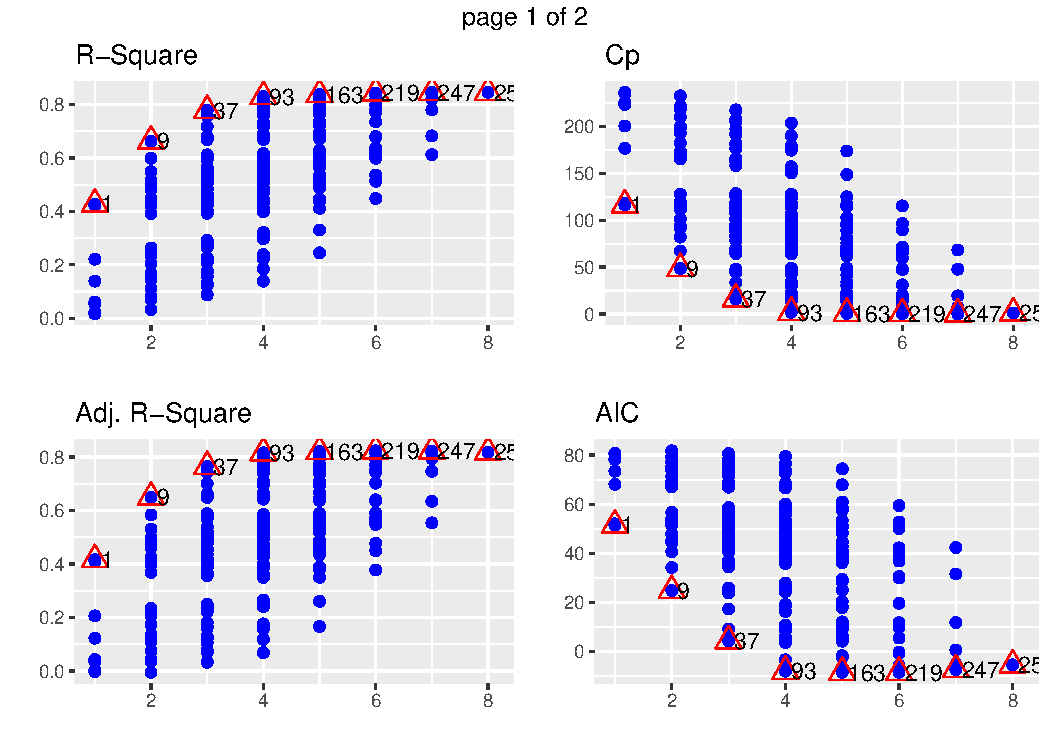
\includegraphics{MLG2_files/figure-latex/surgicalFitAllPlot-1} 

}

\caption{Valores de los criterios de selección calculados para cada uno de todos los posibles modelos.}\label{fig:surgicalFitAllPlot-1}
\end{figure}
\begin{figure}

{\centering 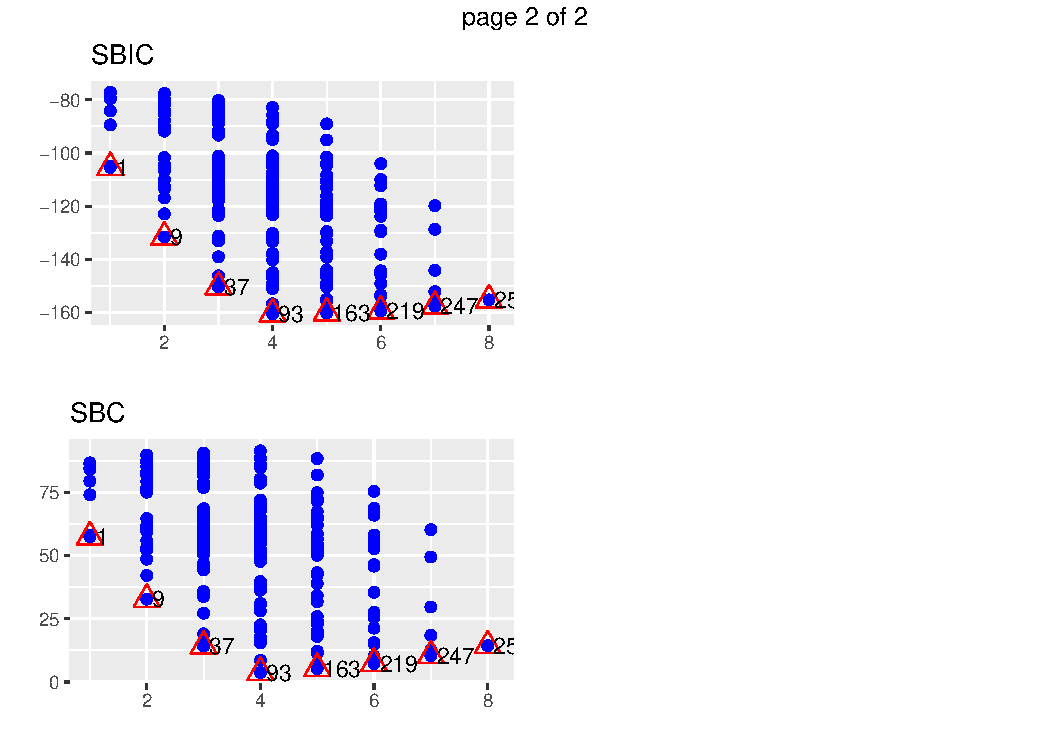
\includegraphics{MLG2_files/figure-latex/surgicalFitAllPlot-2} 

}

\caption{Valores de los criterios de selección calculados para cada uno de todos los posibles modelos.}\label{fig:surgicalFitAllPlot-2}
\end{figure}

Teniendo en cuenta esto, con la función \texttt{ols\_step\_best\_subset()} selecciona el mejor modelo para cada subconjunto de número de covariables basándose en los diferentes criterios:

\begin{Shaded}
\begin{Highlighting}[]
\FunctionTok{ols\_step\_best\_subset}\NormalTok{(mod.surgical.completo)}
\end{Highlighting}
\end{Shaded}

\begin{verbatim}
##                            Best Subsets Regression                           
## -----------------------------------------------------------------------------
## Model Index    Predictors
## -----------------------------------------------------------------------------
##      1         enzyme_test                                                    
##      2         pindex enzyme_test                                             
##      3         pindex enzyme_test alc_heavy                                   
##      4         bcs pindex enzyme_test alc_heavy                               
##      5         bcs pindex enzyme_test gender alc_heavy                        
##      6         bcs pindex enzyme_test age gender alc_heavy                    
##      7         bcs pindex enzyme_test age gender alc_mod alc_heavy            
##      8         bcs pindex enzyme_test liver_test age gender alc_mod alc_heavy 
## -----------------------------------------------------------------------------
## 
##                                                    Subsets Regression Summary                                                   
## --------------------------------------------------------------------------------------------------------------------------------
##                        Adj.        Pred                                                                                          
## Model    R-Square    R-Square    R-Square      C(p)        AIC        SBIC         SBC       MSEP      FPE       HSP       APC  
## --------------------------------------------------------------------------------------------------------------------------------
##   1        0.4273      0.4162      0.3496    117.4783    51.4343    -105.4395    57.4013    7.6160    0.1463    0.0028    0.6168 
##   2        0.6632      0.6500      0.6044     50.4918    24.7668    -131.5971    32.7228    4.5684    0.0893    0.0017    0.3765 
##   3        0.7780      0.7647      0.7291     18.9015     4.2432    -150.4023    14.1881    3.0718    0.0610    0.0012    0.2575 
##   4        0.8299      0.8160      0.7863      5.7340    -8.1306    -160.5329     3.8033    2.4030    0.0486     9e-04    0.2048 
##   5        0.8375      0.8205      0.7828      5.5282    -8.5803    -160.2288     5.3426    2.3453    0.0482     9e-04    0.2032 
##   6        0.8435      0.8235      0.7836      5.7725    -8.6129    -159.4064     7.2990    2.3077    0.0482     9e-04    0.2032 
##   7        0.8460      0.8226      0.7807      7.0288    -7.4974    -157.6344    10.4035    2.3207    0.0492    0.0010    0.2076 
##   8        0.8461      0.8187      0.7711      9.0000    -5.5320    -155.2573    14.3579    2.3719    0.0511    0.0010    0.2154 
## --------------------------------------------------------------------------------------------------------------------------------
## AIC: Akaike Information Criteria 
##  SBIC: Sawa's Bayesian Information Criteria 
##  SBC: Schwarz Bayesian Criteria 
##  MSEP: Estimated error of prediction, assuming multivariate normality 
##  FPE: Final Prediction Error 
##  HSP: Hocking's Sp 
##  APC: Amemiya Prediction Criteria
\end{verbatim}

A partir de estos resultados, y con la ayuda de expertos en el tema, se puede hacer una selección del mejor modelo para hacer las predicciónes.

\hypertarget{algoruxedtmos-de-selecciuxf3n}{%
\subsubsection{Algorítmos de selección}\label{algoruxedtmos-de-selecciuxf3n}}

Para el proceso de selección, la mejor opción es evaluar todos los posibles modelos. Sin embargo, en la presencia de muchas posibles covariables este proceso puede requerir una carga computacional muy alta. Por esta razón, se han desarrollado varios algoritmos para evaluar solo un subconjunto de modelos agregando o eliminando covariables una a la vez.

\hypertarget{selecciuxf3n-hacia-delante-forward-selection}{%
\paragraph{Selección hacia delante (forward selection)}\label{selecciuxf3n-hacia-delante-forward-selection}}

Este algoritmo parte del modelo sin ninguna covariable (es decir, solo el intercepto) y el ajuste ``óptimo'\,' se encuentra ingresando covariables una a la vez basándose en algún criterio (por ejemplo AIC).

La primera covariable se escoge luego de ajustar los \((p-1)\) modelos simples con cada uno de los regresores. Por ejemplo, seleccionado la covariable que proporciona el mejor AIC.

Luego se ajustan los modelos combinando la covariable previamente seleccionada con cada una de los restantes \((p-2)\) regresores. Si el mejor ajuste con dos covariables proporcina un menor AIC que en el paso anterior, continuamos seleccinando la tercer covariable de la misma forma.

El algoritmo continua seleccionando covariables hasta que se satisface un criterio de parada (por ejemplo, hasta que el AIC aumente).

\hypertarget{selecciuxf3n-hacia-atruxe1s-backward-selection}{%
\paragraph{Selección hacia atrás (backward selection)}\label{selecciuxf3n-hacia-atruxe1s-backward-selection}}

Con este algoritmo se empieza evaluando el modelo con todas las covariables candidatas y se van eliminando covariables una a una hasta que un criterio de parada se satisface (por ejemplo, hasta que el AIC aumenta).

\hypertarget{selecciuxf3n-por-segmentos-stepwise-selection}{%
\paragraph{Selección por segmentos (stepwise selection)}\label{selecciuxf3n-por-segmentos-stepwise-selection}}

Aquí se siguen los mismos pasos que la selección hacia delante. Pero en cada paso se evalúan de nuevo los candidatos que ya habían ingresado en el modelo. Por lo tanto, una covariable que ya esté en el modelo puede ser eliminada en algún paso posterior.

\hypertarget{unidad-quiruxfargica-1}{%
\paragraph{Unidad quirúrgica}\label{unidad-quiruxfargica-1}}

Consideremos el modelo anterior adicionando las interacciones de las covariables continuas con las categóricas:
\begin{equation}
\begin{split}
\log y_{i} =& \beta_{0}+\mbox{bcs}_{i}\beta_{1} + \mbox{pindex}_{i}\beta_{2}+ \mbox{enzyme}_{i}\beta_{3} +  \mbox{liver}_{i}\beta_{4} + \mbox{age}_{i}\beta_{5} +  \mbox{gender}_{i}\beta_{6}+ \mbox{alc_mod}_{i}\beta_{7} + \\ &  \mbox{alc_heavy}_{i}\beta_{8} \mbox{bcs}_{i}\mbox{gender}_{i}\beta_{9} + \mbox{pindex}_{i}\mbox{gender}_{i}\beta_{10} + \mbox{enzyme}_{i}\mbox{gender}_{i}\beta_{11} + \mbox{liver}_{i}\mbox{gender}_{i}\beta_{12}  + \\ & \mbox{age}_{i}\mbox{gender}_{i}\beta_{13} + \mbox{bcs}_{i}\mbox{alc_mod}_{i}\beta_{14} + \mbox{pindex}_{i}\mbox{alc_mod}_{i}\beta_{15} + \mbox{enzyme}_{i}\mbox{alc_mod}_{i}\beta_{16} +  \\ & \mbox{liver}_{i}\mbox{alc_mod}_{i}\beta_{17} + \mbox{age}_{i}\mbox{alc_mod}_{i}\beta_{18} + \mbox{bcs}_{i}\mbox{alc_heavy}_{i}\beta_{19} + \mbox{pindex}_{i}\mbox{alc_heavy}_{i}\beta_{20} + \\ & \mbox{enzyme}_{i}\mbox{alc_heavy}_{i}\beta_{21} + \mbox{liver}_{i}\mbox{alc_heavy}_{i}\beta_{22} + \mbox{age}_{i}\mbox{alc_heavy}_{i}\beta_{23} + \varepsilon_{i}.
\end{split}
\nonumber
\end{equation}
En este caso tenemos \(2^{23}=8'388,608\) posibles modelos. Lo que hace que sea difícil ajustarlos todos (aunque es posible usando la librería \texttt{leaps}). Por lo tanto, vamos a utilizar los algortimos de selección.

\textbf{Selección hacia delante}. Podemos utilizar la función \texttt{ols\_step\_forward\_aic} de la librería \texttt{olsrr}:

\begin{Shaded}
\begin{Highlighting}[]
\NormalTok{mod.surgical.completo2 }\OtherTok{=} \FunctionTok{lm}\NormalTok{(}\FunctionTok{log}\NormalTok{(y)}\SpecialCharTok{\textasciitilde{}}\NormalTok{bcs}\SpecialCharTok{*}\NormalTok{gender}\SpecialCharTok{+}\NormalTok{pindex}\SpecialCharTok{*}\NormalTok{gender}\SpecialCharTok{+}\NormalTok{enzyme\_test}\SpecialCharTok{*}\NormalTok{gender}\SpecialCharTok{+}\NormalTok{liver\_test}\SpecialCharTok{*}\NormalTok{gender}\SpecialCharTok{+}\NormalTok{age}\SpecialCharTok{*}\NormalTok{gender}\SpecialCharTok{+}\NormalTok{ bcs}\SpecialCharTok{*}\NormalTok{alc\_mod}\SpecialCharTok{+}\NormalTok{pindex}\SpecialCharTok{*}\NormalTok{alc\_mod}\SpecialCharTok{+}\NormalTok{enzyme\_test}\SpecialCharTok{*}\NormalTok{alc\_mod}\SpecialCharTok{+}\NormalTok{liver\_test}\SpecialCharTok{*}\NormalTok{alc\_mod}\SpecialCharTok{+}\NormalTok{age}\SpecialCharTok{*}\NormalTok{alc\_mod}\SpecialCharTok{+}\NormalTok{bcs}\SpecialCharTok{*}\NormalTok{alc\_heavy}\SpecialCharTok{+}\NormalTok{pindex}\SpecialCharTok{*}\NormalTok{alc\_heavy}\SpecialCharTok{+}\NormalTok{enzyme\_test}\SpecialCharTok{*}\NormalTok{alc\_heavy}\SpecialCharTok{+}\NormalTok{liver\_test}\SpecialCharTok{*}\NormalTok{alc\_heavy}\SpecialCharTok{+}\NormalTok{age}\SpecialCharTok{*}\NormalTok{alc\_heavy,}\AttributeTok{data=}\NormalTok{surgical)}
\NormalTok{res }\OtherTok{=}\FunctionTok{ols\_step\_forward\_aic}\NormalTok{(mod.surgical.completo2,}\AttributeTok{details =}\NormalTok{ F)}
\end{Highlighting}
\end{Shaded}

Con el argumento \texttt{details\ =\ T} se puede ver la selección con más detalle. Usando este algoritmo el modelo óptimo es:
\begin{equation}
\begin{split}
\log y_{i} =& \beta_{0} + \mbox{bcs}_{i}\beta_{1} + \mbox{pindex}_{i}\beta_{2} + \mbox{enzyme}_{i}\beta_{3} + \mbox{age}_{i}\beta_{4} + \mbox{gender}_{i}\beta_{5} + \\
&\mbox{gender}_{i}\mbox{pindex}_{i}\beta_{6} + \mbox{gender}_{i}\mbox{enzyme}_{i}\beta_{7} + \mbox{bcs}_{i}\mbox{alc_heavy}_{i}\beta_{8} + \varepsilon_{i}.
\end{split}
\nonumber
\end{equation}

\textbf{Selección hacia atrás}. Podemos utilizar la función \texttt{ols\_step\_backward\_aic} de la librería \texttt{olsrr}:

\begin{Shaded}
\begin{Highlighting}[]
\FunctionTok{ols\_step\_backward\_aic}\NormalTok{(mod.surgical.completo2,}\AttributeTok{details =}\NormalTok{ F)}
\end{Highlighting}
\end{Shaded}

\begin{verbatim}
## 
## 
##                         Backward Elimination Summary                         
## ---------------------------------------------------------------------------
## Variable                   AIC       RSS     Sum Sq     R-Sq      Adj. R-Sq 
## ---------------------------------------------------------------------------
## Full Model                -9.135    1.058    11.747    0.91740      0.85408 
## age:alc_heavy            -11.134    1.058    11.747    0.91740      0.85878 
## alc_heavy                -13.133    1.058    11.747    0.91740      0.86319 
## bcs:alc_mod              -15.057    1.059    11.745    0.91728      0.86715 
## age:alc_mod              -16.852    1.063    11.741    0.91697      0.87057 
## gender:pindex            -18.639    1.067    11.737    0.91664      0.87377 
## alc_mod                  -19.980    1.080    11.724    0.91562      0.87577 
## enzyme_test:alc_heavy    -20.698    1.106    11.698    0.91359      0.87622 
## liver_test:alc_heavy     -20.988    1.142    11.662    0.91081      0.87560 
## pindex:alc_heavy         -22.223    1.158    11.646    0.90954      0.87706 
## pindex:alc_mod           -22.957    1.186    11.619    0.90739      0.87729 
## bcs:gender               -22.981    1.230    11.575    0.90394      0.87583 
## gender:age               -23.038    1.275    11.529    0.90042      0.87434 
## gender:liver_test        -23.549    1.311    11.494    0.89764      0.87383 
## age                      -23.745    1.355    11.449    0.89416      0.87251 
## ---------------------------------------------------------------------------
\end{verbatim}

Por lo tanto, el modelo seleccionado es:
\begin{equation}
\begin{split}
\log y_{i} =& \beta_{0} + \mbox{bcs}_{i}\beta_{1} + \mbox{pindex}_{i}\beta_{2} + \mbox{enzyme}_{i}\beta_{3} + \mbox{gender}_{i}\beta_{4} + \mbox{liver}_{i}\beta_{5} + \\
& \mbox{gender}_{i}\mbox{enzyme}_{i}\beta_{6} + \mbox{enzyme}_{i}\mbox{alc_mod}_{i}\beta_{7} + \mbox{liver}_{i}\mbox{alc_mod}_{i}\beta_{8} + \mbox{liver}_{i}\mbox{gender}_{i}\beta_{9} \varepsilon_{i}.
\end{split}
\nonumber
\end{equation}
Con este algoritmo no se considera la edad del paciente pero si la función hepática y otras interacciones.

\textbf{Selección por segmentos}. Aquí tenemos la función \texttt{ols\_step\_both\_aic} de la librería \texttt{olsrr}:

\begin{Shaded}
\begin{Highlighting}[]
\FunctionTok{ols\_step\_both\_aic}\NormalTok{(mod.surgical.completo2,}\AttributeTok{details =}\NormalTok{ F)}
\end{Highlighting}
\end{Shaded}

\begin{verbatim}
## 
## 
##                                    Stepwise Summary                                   
## ------------------------------------------------------------------------------------
## Variable               Method       AIC       RSS     Sum Sq     R-Sq      Adj. R-Sq 
## ------------------------------------------------------------------------------------
## enzyme_test           addition     51.434    7.334     5.471    0.42725      0.41624 
## pindex                addition     24.767    4.313     8.492    0.66318      0.64997 
## bcs:alc_heavy         addition     -3.014    2.485    10.320    0.80596      0.79432 
## bcs                   addition     -9.430    2.126    10.678    0.83396      0.82041 
## gender:pindex         addition    -10.781    1.998    10.806    0.84395      0.82770 
## gender:enzyme_test    addition    -19.676    1.633    11.171    0.87246      0.85618 
## gender                addition    -23.040    1.479    11.326    0.88452      0.86695 
## gender:pindex         removal     -23.631    1.518    11.287    0.88147      0.86634 
## age                   addition    -25.088    1.424    11.381    0.88882      0.87190 
## ------------------------------------------------------------------------------------
\end{verbatim}

Note que este método sigue los mismos pasos que la selección hacia delante hasta el paso 8 donde se elimina la interacción entre el índice de pronostico y el genero. Por lo que aquí obtenemos el siguiente modelo:

\begin{equation}
\begin{split}
\log y_{i} =& \beta_{0} + \mbox{bcs}_{i}\beta_{1} + \mbox{pindex}_{i}\beta_{2} + \mbox{enzyme}_{i}\beta_{3} + \mbox{age}_{i}\beta_{4} + \mbox{gender}_{i}\beta_{5} + \\
& \mbox{gender}_{i}\mbox{enzyme}_{i}\beta_{6} + \mbox{bcs}_{i}\mbox{alc_heavy}_{i}\beta_{7} + \varepsilon_{i}.
\end{split}
\nonumber
\end{equation}

Dado que los algoritmos hacen la busqueda del modelo ``óptimo'\,' evaluando diferentes subconjuntos de covariables, se obtuvieron diferentes ajustes. Si observamos el AIC de las tres opciones, el modelo obtenido con el algoritmo stepwise presenta el mejor resultado.

  \bibliography{ModeloLineal.bib}

\end{document}
